%\documentclass[a4paper,12pt]{article}  % standard LaTeX, 12 point type
\documentclass[12pt, a4paper, table]{book}

\usepackage{algpseudocode}
\usepackage{algorithm}
\usepackage{algorithmicx}

\usepackage{geometry}
\usepackage{amsfonts,latexsym}
\usepackage{amsthm}
\usepackage{amssymb}
\usepackage[utf8]{inputenc} % Кодировка
\usepackage[english,russian]{babel} % Многоязычность
\usepackage{mathtools}
\usepackage{hyperref}
\usepackage{tikz}
\usepackage{dsfont}
\usepackage{multicol}
\usepackage[bb=boondox]{mathalfa}

\usetikzlibrary{fit,calc,automata,positioning}

\theoremstyle{definition}
\newtheorem{definition}{Определение}[section]
\newtheorem{example}{Пример}[section]
\newtheorem{theorem}{Теорема}[section]
\newtheorem{proposition}[theorem]{Proposition}
\newtheorem{lemma}[theorem]{Лемма}
\newtheorem{corollary}[theorem]{Corollary}
\newtheorem{conjecture}[theorem]{Conjecture}
\newtheorem{note}[theorem]{Утверждение}


% unnumbered environments:

\theoremstyle{remark}
\newtheorem*{remark}{Remark}
%\newtheorem*{notation}{Notation}

\setlength{\parskip}{5pt plus 2pt minus 1pt}
%\setlength{\parindent}{0pt}


\algtext*{EndWhile}% Remove "end while" text
\algtext*{EndIf}% Remove "end if" text
\algtext*{EndFor}% Remove "end for" text
\algtext*{EndFunction}% Remove "end function" text


\usepackage{color}
\usepackage{listings}
\usepackage{caption}
\usepackage{graphicx}
\usepackage{ucs}

\graphicspath{{pics/}}

%\geometry{left=2cm}
%\geometry{right=1.5cm}
%\geometry{top=2cm}
%\geometry{bottom=2cm}




%\lstnewenvironment{algorithm}[1][]
%{
%    \lstset{
%        frame=tB,
%        numbers=left,
%        mathescape=true,
%        numberstyle=\small,
%        basicstyle=\small,
%        inputencoding=utf8,
%        extendedchars=\true,
%        keywordstyle=\color{black}\bfseries,
%        keywords={,function, procedure, return, datatype, function, in, if, else, for, foreach, while, denote, do, and, then, assert,}
%        numbers=left,
%        xleftmargin=.04\textwidth,
%        #1 % this is to add specific settings to an usage of this environment (for instnce, the caption and referable label)
%    }
%}
%{}

\newcommand{\tab}[1][0.3cm]{\ensuremath{\hspace*{#1}}}

\newcommand{\rvline}{\hspace*{-\arraycolsep}\vline\hspace*{-\arraycolsep}}

\newcommand{\derives}[1][*]{\xRightarrow[]{#1}}
\newcommand{\first}[1][1]{\textsc{first}_{#1}}
\newcommand{\follow}[1][1]{\textsc{follow}_{#1}}

\setcounter{MaxMatrixCols}{20}


\tikzset{
%->, % makes the edges directed
%>=stealth’, % makes the arrow heads bold
node distance=4cm, % specifies the minimum distance between two nodes. Change if necessary.
%every state/.style={thick, fill=gray!10}, % sets the properties for each ’state’ node
initial text=$ $, % sets the text that appears on the start arrow
}

\tikzstyle{symbol_node} = [shape=rectangle, rounded corners, draw, align=center]

\tikzstyle{r_state} = [shape=rectangle, draw, minimum size=0.2cm]

\tikzstyle{prod_node} = [shape=rectangle, draw, align=center]

\tikzset{
    between/.style args={#1 and #2}{
         at = ($(#1)!0.5!(#2)$)
    }
}

%every node/.style = {shape=rectangle, rounded corners,
%      draw, align=center,
%      top color=white, bottom color=blue!20}

\newcommand{\bfgray}[1]{\cellcolor{lightgray}\textbf{#1}}

\newenvironment{scaledalign}[4]
  {
    \begingroup
    #1
    \setlength\arraycolsep{#2}
    \renewcommand{\arraystretch}{#3}
    \begin{center}
    \begin{equation}
    \begin{aligned}
    #4
  }
  {
    \end{aligned}
    \end{equation}
    \end{center}
    \endgroup
  }

\title{Приложения теории формальных языков и синтаксического анализа}
\author{Семён Григорьев}
\date{\today}

\begin{document}
\maketitle
\newpage
\tableofcontents
\newpage

\chapter*{Список авторов}
%\begin{multicols}{2}
    \begin{itemize}
        \item \textbf{Семён Григорьев} \\
              Санкт-Петербургский государственный университет, Университетская набережная, 7/9, Санкт-Петербург, 199034, Россия \\
              \url{s.v.grigoriev@spbu.ru}\\
              \\
              JetBrains Research, Приморский проспект 68-70, здание 1, Санкт-Петербург, 197374, Россия \\
              \url{semyon.grigorev@jetbrains.com}


        \item \textbf{Екатерина Вербицкая} \\
%              Санкт-Петербургский государственный университет \\
%              Университетская набережная, 7/9 \\
%              Санкт-Петербург, 199034, Россия \\
%             \url{s.v.grigoriev@spbu.ru}\\
%              \\
              JetBrains Research, Приморский проспект 68-70, здание 1, Санкт-Петербург, 197374, Россия \\
              \url{ekaterina.verbitskaya@jetbrains.com}
              

        \item \textbf{Дмитрий Кутленков} \\
              Санкт-Петербургский государственный университет, Университетская набережная, 7/9, Санкт-Петербург, 199034, Россия \\
              \url{kutlenkov.dmitri@gmail.com}
              
    \end{itemize}
%\end{multicols}


\section{Introduction}

Context-Free Path Querying (CFPQ) is an actively developed area in graph database analysis.
CFPQ is also used for static code analysis~\cite{Reps,10.1145/193173.195287,Zheng}, RDF querying~\cite{10.1007/978-3-319-46523-4_38,MEDEIROS201975}, biological data analysis~\cite{cfpqBio}.

Most of research is focused on developping algorithms for CFPQ evaluation~\cite{hellingsRelational,ward2008distributed,cfpqBio,MEDEIROS201975,Azimov:2018:CPQ:3210259.3210264,Grigorev:2017:CPQ:3166094.3166104}, whereas specification languages for context-free queries are not investigated enough.
Best to our knowledge, only one extension for Sparql supports context-free constarints: cfSPARQL~\cite{10.1007/978-3-319-46523-4_38}.
There is also a proposal for CFPQ as a part of Cypher\footnote{Proposal with path pattern syntax for openCypher: \url{https://github.com/thobe/openCypher/blob/rpq/cip/1.accepted/CIP2017-02-06-Path-Patterns.adoc}.
It is shown that context-free constraints can be expressed with the proposed syntax. Access date: 30.03.2020} language, but there is no implementation for it yet.
We believe that more research should be conducted on the specification languages fo context-free constraints in graph querying.

It is worth noting that graph analysis is often only a part of a more complex system, usually implemented in a general-purpose language.
Since a graph query language is unsuitable to implement a whole system, there should be means of integration of them into general-purpose programming languages.
There are many ways to integrate them ranging from creating graph queries from string values of a general-purpose language to implementing a special embedded domain specific language, and even more sophisticated.

Although simple, the string manipulating approach does not provide a developper with any safety guarantees.
There is no way to ensure that a string generated by an application is a valid query or, in case it is not, to provide any feedback.
This makes string manipulating technique error prone, the code --- unclear and hard to maintain.

Safety of an embedded DSL entirely depends on its implementation.
Some general-purpose languages with powerfull type systems (such as \haskell{}, \ocaml{} or \scala{}) or the ones supporting hygienic macros (such as \scheme{} or \rust{}) facilitate creating safe and reliable DSLs.
Still, they typically lack full support of a development environment: it may be harder to debug queries or issues with composability may arise.

There is a general trend towards imposing more restricting type systems on programming languages.
Among many others are typing annotations for \python{} and \typescript{} code and nullability checks in \kotlin{}.
Typing graphs and query languages improves  readability and simplifies maintainance~\cite{10.1145/2076623.2076653}.

Parser combinators are the answer to the integration of parsing into a general-purpose programming language.
Recursive descend parsers are encoded as functions of the host language, while grammar constructions such as sequencing and choice are implemented as higher-order functions.
This idea was first introduced in~\cite{burge} and further developped in numerous works.
Notable development is monadic parser combinators~\cite{hutton1996monadic}.
In this approach, one can not only parse the input, but simultaneously run semantics calculation if parsing succeeds.
Paper~\cite{izmaylova2016practical} proposed the first monadic parser combinator library which solves the long-standing problem of inability to handle ambiguous and left-recursive grammars.
A library for graph querying was developped~\cite{10.1145/3241653.3241655} based on this work.
The core idea is to use generalized parser combinators as both a way to formulate a query and to execute it.
This approach inherits benefits of combinatory parsing: ease of code reuse, type safety guaranteed by the host language and, since the parser is simply a function, the integrated development support.

Besides integration, it can compute both the single-source and all pairs semantics, as well as execute user actions.
The~single-source semantics is relevant to many real-world applications, including manual data analysis.
It also may be less time-intensive, since on average it needs to expore only a subgraph of the input graph.
Many querying algorithms are only capable to compute all pairs reachability which makes them unsuitable for some applications.

In this paper we make the following contributions.
\begin{itemize}
  \item We demonstrate how to use combinatory-based graph querying on example.
  \item We illustrate such features of the approach as type-safety, flexibility (composability and generics), IDE support and computing user-defined actions.
  \item We evaluate single-source context-free path querying on some real-world RDFs.
  \begin{itemize}
    \item Based on our evaluation, the most common case in RDF context-free querying is when the number of paths in the answer set is big, but they are small.
    \item We demonstrate that the single-source CFPQ can feasibly be used to evaluate such queries.
    \item We conclude that there is a need for a further detailed analysis of both theoretical time and space complexity of single-source CFPQ.
  \end{itemize}
\end{itemize}

%\chapter[x]{Некоторые понятия линейной алгебры\footnote{Неообходимо понимать, что, с одной строны, в данном разделе рассматриваются самые базовыепонятия, которые даются практически в любом учебнике алгебры. С другой же стороны, определения данных понятий оказываются весьма вариативными и часто вызывают дискуссии. Напрмиер, интересный анализ тонкостей определения группы можно найти в первом и втором параграфах первого раздела книги Николая Александровича Вавилова ``Конкретная теория групп''~\cite{VavilovGroups}. Мы же дадим определения, удобные для дальнейшего изложения материала.}}\label{chpt:LinAlIntro}

При изложении ряда алгоритмов будут активно использоваться некоторые понятия и инструмены линейной алгебры, такие как моноид, полукольцо или матрица.
В данном разделе необходимые понятия будут определены и приведены некоторые примеры соответствующих конструкций. Для более глубокого изучения материала рекомендуются соответствующие разделы алгебры.

$$
\oplus
\otimes
\mathbb{1}
\mathbb{0}
$$

\section{Бинарные операции и их свойства}


Введём понятие \textit{бинарной операции} и рассмотрим некоторые её свойства, такие как \textit{коммутативность} и \textit{ассоциативность}.

\begin{definition}[Двухместная функция] Функцию, принимающую два аргумента, $f: S \times K \to Q$ будем называть двухместной или функцией арности два.
Для запси таких функций будем использовать типичную нотацию: $c = f(a,b)$.
\end{definition}


\begin{definition}[Бинарная операция] 
Бинарная операция --- это двухместная функция, от которой дополнительно требуется, чтобы оба аргумента и результат лежали в одном и том же множестве: $f: S \times S \to S$. В таком случае говорят, что бинарная операция определена на некотором множестве $S$. Для обозначения произвольной бинарной операции будем использовать символ $\circ$ и пользоваться инфиксной нотацией для записи: $c = a \circ b$.
\end{definition}




\begin{definition}[Внешняя бинарная операция]
Внешняя бинарная операция --- это бинарная операция, у которой аргументы лежат в разных множествах, при этом результат --- в одном из этих множеств. Иными словами $\circ: K \times S \to S$, где $K$ может быть не равно $S$  --- внешняя бинарная операция.
\end{definition}


Необходимо помнить, что как функции, так и бинарные операции, могут быть частично определёнными (частичные функции, частичные бинарные операции). Типичным примером частично определённой бинарной операции является деление на целых числах: она не определена, если второй аргумент равен нулю.


Бинарные операции могут обладать некоторыми дополнительными свойствами, такими как \textit{коммутативность} или \textit{ассоциативность}, позволяющими преобразовывать выражения, составленные с использованием этих операций.


\begin{definition}[Коммутативность]
Бинарная операция $\circ : S \times S \to S$ называется коммутативной, если для любых  $x_1 \in S, x_2 \in S$ верно, что  $x_1 \circ x_2 = x_2 \circ x_1$.
\end{definition}

\begin{example} Рассмотрим несколько примеров коммутативных и некоммутативных операций.
	\begin{itemize}
		\item Опреация сложения на целых числах $+$ является коммутативной: известный ещё со школы перестановочный закон сложения.
		\item Операция конкатенации на строках $+$ не является коммутативной: $$``ab" + ``c" \ = ``abc" \neq ``c" + ``ab" \ = ``cab".$$
		\item Операция умножения на целых числах является коммутативной: известный ещё со школы перестановочный закон умножения.
		\item Операция умножения матриц (над целыми числами) $\cdot$ не является коммутативной:
		$$\begin{pmatrix} 
		1 & 1 \\ 0 & 0
		\end{pmatrix}
		\cdot
		\begin{pmatrix} 
		0 & 0 \\ 1 & 1
		\end{pmatrix}
		=
		\begin{pmatrix} 
		1 & 1 \\ 0 & 0
		\end{pmatrix}
		\neq
		\begin{pmatrix} 
		0 & 0 \\ 1 & 1
		\end{pmatrix}
		\cdot
		\begin{pmatrix} 
		1 & 1 \\ 0 & 0
		\end{pmatrix}
		=
		\begin{pmatrix} 
		0 & 0 \\ 1 & 1
		\end{pmatrix}
		.$$
	\end{itemize}
\end{example}

\begin{definition}[Ассоциативность]
Бинарная операция $\circ : S \times S \to S$ называется ассоциативной, если для любых  $x_1 \in S, x_2 \in S, x_3 \in S$ верно, что  $(x_1 \circ x_2) \circ x_3 = x_1 \circ (x_2 \circ x_3)$. Иными словами, для ассоциативной операции результат вычислений не зависит от порядка применения операций.
\end{definition}

\begin{example} Рассмотрим несколько примеров ассоциативных и неассоциативных операций.
	\begin{itemize}
		\item Опреация сложения на целых числах $+$ является ассоциативной.
		\item Операция конкатенации на строках $+$ является ассоциативной: $$``ab" + ``c" \ = ``abc" \neq ``c" + ``ab" \ = ``cab".$$
		\item Операция умножения на целых числах является ассоциативной.
		\item Операция возведения в степень (над целыми числами) $\hat{\mkern6mu}$ не является ассоциативной:
		$$(2\hat{\mkern6mu}2)\hat{\mkern6mu}3 = 4 \hat{\mkern6mu} 3 = 64 \neq 2\hat{\mkern6mu}(2\hat{\mkern6mu}3) = 2 \hat{\mkern6mu} 8  = 256.$$
	\end{itemize}
\end{example}


\begin{definition}[дистрибутивность]
!!!
\end{definition}

\begin{definition}[идемпотентность]
!!!
\end{definition}

\begin{definition}[Нейтральный элемент]
Пусть есть коммутативная бинарная операция $\circ$ на множестве $S$. Говорят, что $x\in S$ является нейтарльным элементом по операции $\circ$, если для любого $y\in S$ верно, что $x \circ y = y \circ x = y$. Если бинарная операция не является коммутативной, то можно пределить \textit{нейтральный слева} и \textit{нейтральный справа} элементы по аналогии.
\end{definition}


\section{Полугруппа}


множество с заданной на нём ассоциативной бинарной операцией $(S,\cdot )$ 


Коммутативная полугруппа


The set of positive integers with addition. (With 0 included, this becomes a monoid.)
The set of integers with minimum or maximum. (With positive/negative infinity included, this becomes a monoid.)
Square nonnegative matrices of a given size with matrix multiplication.
Any ideal of a ring with the multiplication of the ring.
The set of all finite strings over a fixed alphabet $\Sigma$ with concatenation of strings as the semigroup operation — the so-called ``free semigroup over $\Sigma$''. With the empty string included, this semigroup becomes the free monoid over $\Sigma$.


\section{Моноид}


Полугруппа с нейтральным элементом.



\section{Группа}


Непустое множество $G$ с заданной на нём бинарной операцией $*$: $ \mathrm {G} \times \mathrm {G} \rightarrow \mathrm {G}$ называется группой $ (\mathrm {G} ,*)$, если выполнены следующие аксиомы:

ассоциативность: $\forall (a,b,c\in G)\colon (a*b)*c=a*(b*c)$;
наличие нейтрального элемента: $ \exists e\in G\quad \forall a\in G\colon (e*a=a*e=a)$;
наличие обратного элемента: $ \forall a\in G\quad \exists a^{-1}\in G\colon (a*a^{-1}=a^{-1}*a=e)$.

Иными словами, группа --- это моноид с дополнительным требованием наличия обратных элементов.

\begin{definition}[Абелева группа] --- операция коммутативна.
\end{definition}


\section{Полукольцо}

A semiring is a set R equipped with two binary operations + and $\otimes$, called addition and multiplication, such that:[3][4][5]

(R, +) is a commutative monoid with identity element 0:
(a + b) + c = a + (b + c)
0 + a = a + 0 = a
a + b = b + a
(R, $\otimes$) is a monoid with identity element 1:
(a$\otimes$b)$\otimes$c = a$\otimes$(b$\otimes$c)
1$\otimes$a = a$\otimes$1 = a
Multiplication left and right distributes over addition:
a$\otimes$(b + c) = (a$\otimes$b) + (a$\otimes$c)
(a + b)$\otimes$c = (a$\otimes$c) + (b$\otimes$c)
Multiplication by 0 annihilates R:
0$\otimes$a = a$\otimes$0 = 0


\section{Кольцо}


A ring is a set R equipped with two binary operations[a] + (addition) and $\otimes$ (multiplication) satisfying the following three sets of axioms, called the ring axioms[1][2][3]

R is an abelian group under addition, meaning that:
(a + b) + c = a + (b + c) for all a, b, c in R   (that is, + is associative).
a + b = b + a for all a, b in R   (that is, + is commutative).
There is an element 0 in R such that a + 0 = a for all a in R   (that is, 0 is the additive identity).
For each a in R there exists $-a$ in R such that $a + (-a) = 0$   (that is, $-a$ is the additive inverse of a).
R is a monoid under multiplication, meaning that:
(a $\otimes$ b) $\otimes$ c = a $\otimes$ (b $\otimes$ c) for all a, b, c in R   (that is, $\otimes$ is associative).
There is an element 1 in R such that a $\otimes$ 1 = a and 1 $\otimes$ a = a for all a in R   (that is, 1 is the multiplicative identity).[b]
Multiplication is distributive with respect to addition, meaning that:
a $\otimes$ (b + c) = (a $\otimes$ b) + (a $\otimes$ c) for all a, b, c in R   (left distributivity).
(b + c) $\otimes$ a = (b $\otimes$ a) + (c $\otimes$ a) for all a, b, c in R   (right distributivity).


\section{Поле}

\section{Матрицы и вектора}

Вектор

Матрица 

Про матричное произведение, тензорное произведение, ещё что-то.

\section{Вопросы и задачи}
\begin{enumerate}
	\item Привидите примеры некоммутативных операций.
	\item Привидите примеры ситуаций, когда наличие у бинарных операций каких-либо дополнитльных свойств (ассоциативности, коммутативности), позволяет строить более эффективные алгоритмы, чем в общем случае.
\end{enumerate}
\section{Общие сведения теории графов}

основные определения: рёбра, вершины, графы ориентированные, неориентированные, помеченные.

Специальные понятия, необходимые для иложения конкретного материала, будут даны в соответсвующих главах.

Матрицы смежности

\subsection{Транзитивне замыкание графа}

Флойд-Уоршал, матрицы.

Рассуждения про субкубичность.
Про то, что булево полукольцо.


\subsection{Задачи поиска путей}

Достижимость, все пути, один путь.

Про кратчайшие, простые и прочее.

Про классические задачи и классическое сведение к матричным операциям.

Тра-та-та.

\subsection{Вопросы и задачи}
\begin{enumerate}
  \item Реализуйте алгоритм построения транзитивного замыкания через матрицы.
  Реализовать матрицы самим.
  Взять готовую библиотеку матричных операций: CPU, GPGPU.
  \item Реализуйте поиск кратчайших путей через матричные операции.
  Реализовать перемножение матриц самостоятельно.
  Взять готовую библиотеку матричных операций: CPU, GPGPU.
\end{enumerate}

\section{Общие сведения теории формальных языков}

В данной главе мы рассмотрим основные понятия из теории формальных языков, которые пригодятся нам в дальнейшем изложении.

\begin{definition}
\textit{Алфавит} --- это конечное множество.
Элементы этого множества будем называть \textit{символами}.
\end{definition}

Традиционное обозначение для алфавита --- $\Sigma$.
Также мы будем использовать различные прописные буквы латинского алфавита.

Будем считать, что над алфавитом $\Sigma$ всегда определена операция конкатенации $(\cdot): \Sigma^* \times \Sigma^* \to \Sigma^*$.
При записи выражений символ точки (обозначение операции конкатенации) часто будем опускать: $a \cdot b = ab$.

\begin{definition}
\textit{Слово} над алфавитом $\Sigma$ --- это конечная конкатенация символов алфавита $\Sigma$: $\omega = a_0 \cdot a_1 \cdot \ldots \cdot a_m$, где $\omega$ --- слово, а для любого $i$ $a_i \in \Sigma$.
\end{definition}

\begin{definition}
\textit{Слово} над алфавитом $\Sigma$ --- это результат конечной конкатенации символов алфавита $\Sigma$: $\omega = a_0 \cdot a_1 \cdot \ldots \cdot a_m$, где $\omega$ --- слово, а для любого $i$ $a_i \in \Sigma$.
Будем называть $m + 1$ длиной слова и обозначать как $|\omega|$.
\end{definition}

\begin{definition}
\textit{Язык} над алфавитом $\Sigma$ --- это множество слов над алфавитом $\Sigma$.
\end{definition}

Заметим, что язык не обязан быть конечным множеством, в то время как алфавит обязан быть конечным и изучаем мы конечные слова.

Общие способы задать язык.
\begin{itemize}
\item Перечислить все элементы. Такой способ работает только для конечных языков. Перечислить бесконечное множество не получится.
\item Задать генератор --- процедуру, которая возвращает очередное слово языка.
\item Задаьть распознователь --- процедуру, которая по данному слову может определить, принадлежит оно заданному языку ли нет.
\end{itemize}


\subsection{Контекстно-свободные грамматики и языки}

Из всего многообразия нас будут интересовать прежде всего контекстно-свободные грамматики.

\begin{definition}
\textit{Контекстно-свободная грамматика} --- это четвёрка вида $\langle \Sigma, N, P, S \rangle$, где
\begin{itemize}
  \item $\Sigma$ --- это терминальный алфавит;
  \item $N$ --- это нетерминальный алфавит;
  \item $P$ --- это множество правил или продукций, таких что кажая продукция имеет вид $N_i \to \alpha$, где $N_i \in N$ и $\alpha \in \{\Sigma \cup N\}^* \cup {\varepsilon}$;
  \item $S$ --- стартовый нетерминал.
  Отметим, что $\Sigma \cap N = \varnothing$.
\end{itemize}
\end{definition}

\begin{definition}
\textit{Отношение выводимости} на $ $
\end{definition}

\begin{definition}
\textit{Вывод слова в граммтике}
\end{definition}

\begin{definition}
\textit{Левосторонний вывод}
\end{definition}

Аналогично можно определить правосторонний вывод.

\begin{definition}
\textit{Язык $L$, задаваемый граммтикой $G$} ---  это множество свех слов, выводимых в граммтике $G$. иными словами, $L(G) = L(\langle \Sigma, N, P, S \rangle)\{ \omega \mid S \to ^* \omega\}$.
\end{definition}

Неоднозначные граммтики.

Существенно неоднозначные языки.


\subsection{Дерево вывода}
В некоторых случаях не достаточно знать порядок рименения правил.
Необходимо структурное представление вывода цепочки в граммтике.
Таким представлением является \textit{дерево вывода}.
\begin{definition}
Деревом вывода цепочки $\omega$ в граммтике $G=\langle \Sigma, N, S, P \rangle$ называется дерево, удовлетворяющее следующим свойствам.

\begin{enumerate}
  \item Помеченное: метка каждого внутреннего узла --- нетерминал, метка каждого листа --- терминал или $\varepsilon$.
  \item Корневое. Корень помечен стартовым нетерминалом.
  \item Упорядоченное.
  \item В дереве есть узел с меткой $N_i$ и сыновьями $M_j \dots M_k$ тогда и только тогда, когда в грамматике есть правило вида $N_i \to M_j M_k$.
  \item Крона --- цепочка.
\end{enumerate}
\end{definition}

\begin{example}
  Построим дерево вывода цепочки $ababab$ в граммтике $G = \langle \{a,b\}, \{S\}, S, {S \to a \ S \ b \ S, S \to \varepsilon} \rangle$.

  \begin{tikzpicture}[sibling distance=4em,
  every node/.style = {shape=rectangle, rounded corners,
    draw, align=center,
    top color=white, bottom color=blue!20}]]
  \node {S}
    child { node {a} }
    child { node {S}
      child { node {$\varepsilon$}}
    }
    child { node {b} }
    child { node {S}
      child {node {a}}
      child { node {S}
        child { node {$\varepsilon$}}
      }
      child { node {b} }
      child { node {S}
        child {node {a}}
        child {node {S}
          child {node {$\varepsilon$}}
        }
        child {node {b}}
        child {node {S}
          child {node {$\varepsilon$}}
        }
      }
    };
\end{tikzpicture}

\end{example}


\subsection{Нормальная форма Хомского}
\label{section:CNF}

\begin{definition}
Определение НФХ.
\end{definition}

\begin{theorem}
Любую КС граммтику можно преобразовать в НФХ.
\end{theorem}


\subsection{Вопросы и задачи}
\begin{enumerate}
  \item Предъявить несколько выовдов для одной цепочки.
  \item Построить выводы
  \item Построить деревья вывода !!! Перенести из раздела про SPPF
\end{enumerate}

\input{FLPQ}
%\chapter{Регулярные языки}

Регулярные языки, конечные автоматы, взяимные конвертации, замкнутость.

Лемма о накачке

Линейная алгебра для работы с регулярными языками: пересечение, замыкание.



\section{Задача поиска путей с ограничениями в терминах регулярных языков}

Графовая база данных --- автомат.

Задача --- пересечение автоматов.

Линейная алгебра, производные, построение атомата, выяснение существования путей.

\section{Вопросы и задачи}

Построить базу.

Научиться выполнять запросы через линейку. 
\chapter{Контекстно-свободные грамматики и языки}\label{CFG}

Из всего многообразия нас будут интересовать прежде всего контекстно-свободные грамматики.

\begin{definition}
\textit{Контекстно-свободная грамматика} --- это четвёрка вида $\langle \Sigma, N, P, S \rangle$, где
\begin{itemize}
  \item $\Sigma$ --- это терминальный алфавит;
  \item $N$ --- это нетерминальный алфавит;
  \item $P$ --- это множество правил или продукций, таких что каждая продукция имеет вид $N_i \to \alpha$, где $N_i \in N$ и $\alpha \in \{\Sigma \cup N\}^* \cup {\varepsilon}$;
  \item $S$ --- стартовый нетерминал.
  Отметим, что $\Sigma \cap N = \varnothing$.
\end{itemize}
\end{definition}

\begin{example}
Грамматика, задающая язык целых чисел в двоичной записи без лидирующих нулей: $G = \langle \{0, 1, -\}, \{S, N, A\}, P, S \rangle$, где $P$ определено следующим образом:

\[
\begin{array}{rcl}
S& \rightarrow & 0 \mid N \mid - N  \\
N& \rightarrow & 1 A \\
A& \rightarrow & 0 A \mid 1 A  \mid \varepsilon\\
\end{array}
\]
\end{example}

При спецификации грамматики часто опускают множество терминалов и нетерминалов, оставляя только множество правил. При этом нетерминалы часто обозначаются прописными латинскими буквами, терминалы --- строчными, а стартовый нетерминал обозначается буквой~$S$. Мы будем следовать этим обозначениям, если не указано иное.


\begin{definition}\label{def derivability in CFG}
  \textit{Отношение непосредственной выводимости}. Мы говорим, что последовательность терминалов и нетерминалов $\gamma \alpha \delta$ \textit{непосредственно выводится из} $\gamma \beta \delta$ \textit{при помощи правила} $\alpha \rightarrow \beta$ ($\gamma \alpha \delta \Rightarrow \gamma \beta \delta$), если
  \begin{itemize}
    \item $\alpha \rightarrow \beta \in P$
    \item $\gamma, \delta \in \{\Sigma \cup N\}^* \cup {\varepsilon}$
  \end{itemize}
\end{definition}

\begin{definition}
  \textit{Рефлексивно-транзитивное замыкание отношения} --- это наименьшее рефлексивное и транзитивное отношение, содержащее исходное.
\end{definition}

\begin{definition}
\textit{Отношение выводимости} является рефлексивно-транзитивным замыканием отношения непосредственной выводимости
\begin{itemize}
  \item $\alpha \derives \beta$ означает $\exists \gamma_0, \dots \gamma_k: \ \alpha \derives[] \gamma_0 \derives[] \gamma_1 \derives[] \dots \derives[] \gamma_{k-1} \derives[] \gamma_{k} \derives[] \beta$
  \item Транзитивность: $\forall \alpha, \beta, \gamma \in \{\Sigma \cup N\}^* \cup {\varepsilon}: \ \alpha \derives \beta, \beta \derives \gamma \Rightarrow \alpha \derives \gamma$
  \item Рефлексивность: $\forall \alpha \in \{\Sigma \cup N\}^* \cup {\varepsilon}: \ \alpha \derives \alpha$
  \item $\alpha \derives \beta$ --- $\alpha$ выводится из $\beta$
  \item $\alpha \derives[k] \beta$ --- $\alpha$ выводится из $\beta$ за $k$ шагов
  \item $\alpha \derives[+] \beta$ --- при выводе использовалось хотя бы одно правило грамматики
\end{itemize}
\end{definition}


\begin{example}
Пример вывода цепочки $-1101$ в грамматике:

  \[
  \begin{array}{rcl}
  S& \rightarrow & 0 \mid N \mid - N  \\
  N& \rightarrow & 1 A \\
  A& \rightarrow & 0 A \mid 1 A  \mid \varepsilon\\
  \end{array}
  \]

  \[ S \Rightarrow - N \Rightarrow - 1 A \Rightarrow - 1 1 A \derives - 1 1 0 1 A \Rightarrow - 1 1 0 1 \]
\end{example}


\begin{definition}[Вывод слова в грамматике]
Слово $\omega \in \Sigma^*$ \textit{выводимо в грамматике} $\langle \Sigma, N, P, S \rangle$, если существует некоторый вывод этого слова из начального нетерминала $S \derives \omega$.

\end{definition}

\begin{definition}
\textit{Левосторонний вывод}. На каждом шаге вывода заменяется самый левый нетерминал.
\end{definition}

\begin{example}
Пример левостороннего вывода цепочки в грамматике

  \[
    \begin{array}{rcl}
    S& \rightarrow & A A \mid s  \\
    A& \rightarrow & A A \mid B b \mid a \\
    B& \rightarrow & c \mid d
    \end{array}
  \]

  \[ \boldsymbol{S} \derives[] \boldsymbol{A} A \derives[] \boldsymbol{B} b A \derives[] c b \boldsymbol{A} \derives[] c b \boldsymbol{A} A \derives[] c b a \boldsymbol{A} \derives[] c b a a \]
\end{example}

Аналогично можно определить правосторонний вывод.

\begin{definition}
\textit{Язык, задаваемый грамматикой} --- множество строк, выводимых в грамматике $L(G) = \{ \omega \in \Sigma^* \mid S \derives \omega \}$.
\end{definition}

\begin{definition}
  Грамматики $G_1$ и $G_2$ называются \textit{эквивалентными}, если они задают один и тот же язык: $L(G_1) = L(G_2)$
\end{definition}


\begin{example}  Пример эквивалентных грамматик для языка целых чисел в двоичной системе счисления.

  \begin{tabular}{p{0.4\textwidth} | p{0.5\textwidth}}

    \[
      \begin{array}{rcl}
      \Sigma &=& \{ 0, 1, - \} \\
      N &=& \{ S, N, A \} \\~\\
      S& \rightarrow & 0 \mid N \mid - N  \\
      N& \rightarrow & 1 A \\
      A& \rightarrow & 0 A \mid 1 A  \mid \varepsilon\\
      \end{array}
    \]

    &

    \[
      \begin{array}{rcl}
      \Sigma &=& \{ 0, 1, - \} \\
      N &=& \{ S, A \} \\~\\
      S& \rightarrow & 0 \mid 1 A  \mid - 1 A  \\
      A& \rightarrow &  0 A \mid 1 A  \mid \varepsilon\\
      \end{array}
    \]
    \end{tabular}

\end{example}


\begin{definition}
  \textit{Неоднозначная грамматика} --- грамматика, в которой существует 2 и более левосторонних (правосторонних) выводов для одного слова.
\end{definition}

\begin{example}
  Неоднозначная грамматика для правильных скобочных последовательностей

\[
    S \to (S) \mid S S \mid \varepsilon
\]
\end{example}

\begin{definition}
  \textit{Однозначная грамматика} --- грамматика, в которой существует не более одного левостороннего (правостороннего) вывода для каждого слова.
\end{definition}

\begin{example}
  Однозначная грамматика для правильных скобочных последовательностей

\[
    S \to (S)S \mid \varepsilon
\]
\end{example}

\begin{definition}
  \textit{Существенно неоднозначные языки} --- языки, для которых невозможно построить однозначную грамматику.
\end{definition}

\begin{example}
  Пример существенно неоднозначного языка

\[\{a^n b^n c^m \mid n, m \in \mathds{Z}\} \cup \{a^n b^m c^m \mid n,m \in \mathds{Z}\}\]
\end{example}

\section{Дерево вывода}\label{sect:DerivTree}
В некоторых случаях не достаточно знать порядок применения правил.
Необходимо структурное представление вывода цепочки в грамматике.
Таким представлением является \textit{дерево вывода}.
\begin{definition}
Деревом вывода цепочки $\omega$ в грамматике $G=\langle \Sigma, N, S, P \rangle$ называется дерево, удовлетворяющее следующим свойствам.

\begin{enumerate}
  \item Помеченное: метка каждого внутреннего узла --- нетерминал, метка каждого листа --- терминал или $\varepsilon$.
  \item Корневое: корень помечен стартовым нетерминалом.
  \item Упорядоченное.
  \item В дереве может существовать узел с меткой $N_i$ и сыновьями $M_j \dots M_k$ только тогда, когда в грамматике есть правило вида $N_i \to M_j \dots M_k$.
  \item Крона образует исходную цепочку $\omega$.
\end{enumerate}
\end{definition}

\begin{example}
  Построим дерево вывода цепочки $ababab$ в грамматике

  \[ G = \langle \{a,b\}, \{S\}, S, \{S \to a \ S \ b \ S, S \to \varepsilon\} \rangle \]

\begin{center}

    \begin{tikzpicture}[sibling distance=4em,
    every node/.style = {shape=rectangle, rounded corners,
      draw, align=center,
      top color=white, bottom color=blue!20}]]
    \node {S}
      child { node {a} }
      child { node {S}
        child { node {$\varepsilon$}}
      }
      child { node {b} }
      child { node {S}
        child {node {a}}
        child { node {S}
          child { node {$\varepsilon$}}
        }
        child { node {b} }
        child { node {S}
          child {node {a}}
          child {node {S}
            child {node {$\varepsilon$}}
          }
          child {node {b}}
          child {node {S}
            child {node {$\varepsilon$}}
          }
        }
      };
  \end{tikzpicture}
\end{center}

\end{example}

\begin{theorem}
  Пусть $G = \langle \Sigma, N, P, S \rangle$ --- КС-грамматика.
  Вывод $S \derives \alpha$, где $\alpha \in (N \cup \Sigma)^*, \alpha \neq \varepsilon$ существует $\Leftrightarrow$ существует дерево вывода в грамматике $G$ с кроной $\alpha$.
\end{theorem}

\section{Пустота КС-языка}

\begin{theorem}
  Существует алгоритм, определяющий, является ли язык, порождаемый КС грамматикой, пустым.
\end{theorem}

\begin{proof}
  Следующая лемма утверждает, что если в КС языке есть выводимое слово, то существует другое выводимое слово с деревом вывода не глубже количества нетерминалов грамматики.
  Для доказательства теоремы достаточно привести алгоритм, последовательно строящий все деревья глубины не больше количества нетерминалов грамматики, и проверяющий, являются ли такие деревья деревьями вывода.
  Если в результате работы алгоритма не удалось построить ни одного дерева, то грамматика порождает пустой язык.
\end{proof}

\begin{lemma}
  Если в данной грамматике выводится некоторая цепочка, то существует цепочка, дерево вывода которой не содержит ветвей длиннее m, где m --- количество нетерминалов грамматики.
\end{lemma}

\begin{proof}
  Рассмотрим дерево вывода цепочки $\omega$. Если в нем есть 2 узла, соответствующих одному нетерминалу A, обозначим их $n_1$ и $n_2$.

  Предположим, $n_1$ расположен ближе к корню дерева, чем $n_2$.

  $S \derives \alpha A_{n_1} \beta \derives \alpha \omega_1 \beta; S \derives \alpha \gamma A_{n_2} \delta \beta \derives \alpha \gamma \omega_2 \delta \beta$, при этом $\omega_2$ является подцепочкой $\omega_1$.

  Заменим в изначальном дереве узел $n_1$ на $n_2$. Полученное дерево является деревом вывода $\alpha \omega_2 \delta$.

  Повторяем процесс замены одинаковых нетерминалов до тех пор, пока в дереве не останутся только уникальные нетерминалы.

  В полученном дереве не может быть ветвей длины большей, чем m.

  По построению оно является деревом вывода.
\end{proof}


\section{Нормальная форма Хомского}
\label{section:CNF}

\begin{definition}
Контекстно-свободная грамматика $\langle \Sigma, N, P, S\rangle$ находится в \textit{Нормальной Форме Хомского}, если она содержит только правила следующего вида:

\begin{itemize}
  \item $A \to B C \text{, где } A, B, C \in N \text{, S не содержится в правой части правила }$
  \item $A \to a \text{, где } A \in N, a \in \Sigma$
  \item $S \to \varepsilon$
\end{itemize}
\end{definition}

\begin{theorem}
Любую КС грамматику можно преобразовать в НФХ.
\end{theorem}

\begin{proof}
  Алгоритм преобразования в НФХ состоит из следующих шагов:

  \begin{itemize}
    \item Замена неодиночных терминалов
    \item Удаление длинных правил
    \item Удаление $\varepsilon$-правил
    \item Удаление цепных правил
    \item Удаление бесполезных нетерминалов
  \end{itemize}

  То, что каждый из этих шагов преобразует грамматику к эквивалентной, при этом является алгоритмом, доказано в следующих леммах.
\end{proof}

\begin{lemma}
  Для любой КС-грамматики можно построить эквивалентную, которая не содержит правила с неодиночными терминалами.
\end{lemma}

\begin{proof}
  Каждое правило $A \to B_0 B_1 \dots B_k, k \geq 1$ заменить на множество правил:
  \begin{itemize}
    \item $A \to C_0 C_1 \dots C_k$
    \item $\{ C_i \to B_i \mid B_i \in \Sigma, C_i \text{ --- новый нетерминал} \}$
  \end{itemize}
\end{proof}

\begin{lemma}
  Для любой КС-грамматики можно построить эквивалентную, которая не содержит правил длины больше 2.
\end{lemma}

\begin{proof}
  Каждое правило $A \to B_0 B_1 \dots B_k, k \geq 2$ заменить на множество правил:
  \begin{itemize}
    \item $A \to B_0 C_0$
    \item $C_0 \to B_1 C_1$
    \item $\dots$
    \item $C_{k-3} \to B_{k-2} C_{k-2}$
    \item $C_{k-2} \to B_{k-1} B_k$
  \end{itemize}
\end{proof}


\begin{lemma}
  Для любой КС-грамматики можно построить эквивалентную, не содержащую $\varepsilon$-правил.
\end{lemma}

\begin{proof}
  Определим $\varepsilon$-правила:
  \begin{itemize}
    \item $A \to \varepsilon$
    \item $A \to B_0 \dots B_k, \forall i: \ B_i$ --- $\varepsilon$-правило.
  \end{itemize}

  Каждое правило $A \to B_0 B_1 \dots B_k$ заменяем на множество правил, где каждое $\varepsilon$-правило удалено во всех возможных комбинациях.
\end{proof}

\begin{lemma}
  Можно удалить все цепные правила
\end{lemma}

\begin{proof}
  \textit{Цепное правило} --- правило вида $A \to B\text{, где } A, B \in N\\$.
  \textit{Цепная пара} --- упорядоченная пара $(A,B)$, в которой $A\derives B$, используя только цепные правила.
  
  Алгоритм:
  \begin{enumerate}
  \item Найти все цепные пары в грамматике $G$.
  Найти все цепные пары можно по индукции:
  Базис: $(A,A)$ --- цепная пара для любого нетерминала, так как $A\derives A$ за ноль шагов.
  Индукция: Если пара $(A,B_0)$ --- цепная, и есть правило $B_0 \to B_1$, то $(A,B_1)$ --- цепная пара.
  \item Для каждой цепной пары $(A,B)$ добавить в грамматику $G'$ все правила вида $A \to a$, где $B \to a$ --- нецепное правило из $G$.
  \item Удалить все цепные правила
\end{enumerate}
Пусть $G$ --- контекстно-свободная грамматика. $G'$ --- грамматика, полученная в результате применения алгоритма к $G$. Тогда $L(G)=L(G')$.
\end{proof}

\begin{definition}
Нетерминал $A$ называется \textit{порождающим}, если из него может быть выведена конечная терминальная цепочка. Иначе он называется \textit{непорождающим}.
\end{definition}

\begin{lemma}
  Можно удалить все бесполезные (непорождающие) нетерминалы
\end{lemma}

\begin{proof}
  После удаления из грамматики правил, содержащих непорождающие нетерминалы, язык не изменится, так как непорождающие нетерминалы по определению не могли участвовать в выводе какого-либо слова.
  
  Алгоритм нахождения порождающих нетерминалов:
  \begin{enumerate}
  \item Множество порождающих нетерминалов пустое.
  \item Найти правила, не содержащие нетерминалов в правых частях и добавить нетерминалы, встречающихся в левых частях таких правил, в множество.
  \item Если найдено такое правило, что все нетерминалы, стоящие в его правой части, уже входят в множество, то добавить в множество нетерминалы, стоящие в его левой части.
  \item Повторить предыдущий шаг, если множество порождающих нетерминалов изменилось.
\end{enumerate}
В результате получаем множество всех порождающих нетерминалов грамматики, а все нетерминалы, не попавшие в него, являются непорождающими. Их можно удалить.
\end{proof}

\begin{example}
  Приведем в Нормальную Форму Хомского однозначную грамматику правильных скобочных последовательностей: $S \to a S b S \mid \varepsilon$

  Первым шагом добавим новый нетерминал и сделаем его стартовым: 

  \begin{align*}
    S_0 &\to S  \\ 
    S   &\to a S b S \mid \varepsilon
  \end{align*}

  Заменим все терминалы на новые нетерминалы: 

  \begin{align*}
    S_0 &\to S \\ 
    S   &\to L S R S \mid \varepsilon \\ 
    L   &\to a \\ 
    R   &\to b
  \end{align*}

  Избавимся от длинных правил: 

  \begin{align*}
    S_0 &\to S \\ 
    S   &\to L S' \mid \varepsilon \\ 
    S'  &\to S S'' \\ 
    S'' &\to R S \\
    L   &\to a \\ 
    R   &\to b
  \end{align*}

  Избавимся от $\varepsilon$-продукций: 

  \begin{align*}
    S_0 &\to S \mid \varepsilon \\ 
    S   &\to L S' \\ 
    S'  &\to S'' \mid S S'' \\ 
    S'' &\to R   \mid R S \\
    L   &\to a \\ 
    R   &\to b
  \end{align*}

  Избавимся от цепных правил: 

  \begin{align*}
    S_0 &\to L S' \mid \varepsilon \\ 
    S   &\to L S' \\ 
    S'  &\to b \mid R S \mid S S'' \\ 
    S'' &\to b \mid R S \\
    L   &\to a \\ 
    R   &\to b
  \end{align*}
\end{example}

\begin{definition}\label{defn:wCNF}
Контекстно-свободная грамматика $\langle \Sigma, N, P, S\rangle$ находится в \textit{ослабленной Нормальной Форме Хомского}, если она содержит только правила следующего вида:

\begin{itemize}
  \item $A \to B C \text{, где } A, B, C \in N$
  \item $A \to a \text{, где } A \in N, a \in \Sigma$
  \item $A \to \varepsilon \text{, где } A \in N$
\end{itemize}

То есть ослабленная НФХ отличается от НФХ тем, что:
\begin{enumerate}
  \item $\varepsilon$ может выводиться из любого нетерминала
  \item $S$ может появляться в правых частях правил
\end{enumerate}
\end{definition}

\section{Лемма о накачке}

\begin{lemma}
Пусть $L$ --- контекстно-свободный язык над алфавитом $\Sigma$, тогда существует такое $n$, что для любого слова $\omega \in L$, $|\omega| \geq n$ найдутся слова $u,v,x,y,z\in \Sigma^*$, для которых верно: $uvxyz = \omega, vy\neq \varepsilon,|vxy|\leq n$ и для любого $k \geq 0$  $uv^kxy^kz \in L$.
\end{lemma}

Идея доказательства леммы о накачке.

\begin{enumerate}
    \item Для любого КС языка можно найти грамматику в нормальной форме Хомского.
    \item Очевидно, что если брать достаточно длинные цепочки, то в дереве вывода этих цепочек, на пути от корня к какому-то листу обязательно будет нетерминал, встречающийся минимум два раза. Если $m$ --- количество нетерминалов в НФХ, то длины $2^{m+1}$ должно хватить. Это и будет $n$ из леммы.
    \item Возьмём путь, на котором есть хотя бы дважды повторяется некоторый нетерминал. Скажем, это нетерминал  $N_1$. Пойдём от листа по этому пути. Найдём первое появление $N_1$. Цепочка, задаваемая поддеревом для этого узла --- это $x$ из леммы.
    \item Пойдём дальше и найдём второе появление $N_1$. Цепочка, задаваемая поддеревом для этого узла --- это $vxy$ из леммы.
    \item Теперь мы можем копировать кусок дерева между этими повторениями $N_1$ и таким образом накачивать исходную цепочку.
\end{enumerate}

Надо только проверить выполение ограничений на длины.

Нахождение разбиения и пример накачки продемонстрированы на рисунках~\ref{fig:pumping1} и~\ref{fig:pumping2}.

\begin{figure}
\centering
\includegraphics[width=0.5\textwidth]{pics/pumping_tree_1.pdf}
\caption{Разбиение цепочки для леммы о накачке}
\label{fig:pumping1}
\end{figure}

\begin{figure}
\centering
\includegraphics[width=0.5\textwidth]{pics/pumping_tree_2.pdf}
\caption{Пример накачки цепочки с рисунка~\ref{fig:pumping1}}
\label{fig:pumping2}
\end{figure}


Для примера предлагается проверить неконтекстно-свободность языка $L=\{a^nb^nc^n \mid n>0\}$.


\section{Замкнутость КС языков относительно операций}


\begin{theorem}
Контекстно-свободные языки замкнуты относительно следующих операций:
\begin{enumerate}
  \item Объединение: если $L_1$ и $L_2$ --- контекстно-свободные языки, то и $L_3 = L_1 \cup L_2$ --- контекстно-свободный.
  \item Конкатенация: если $L_1$ и $L_2$ --- контекстно-свободные языки, то и $L_3 = L_1 \cdot L_2$ --- контекстно-свободный.
  \item Замыкание Клини: если $L_1$ --- контекстно-свободный, то и $L_2 = \bigcup\limits_{i=0}^{\infty} L_1^i $ --- контекстно-свободный.
  \item Разворот: если $L_1$ --- контекстно-свободный, то и $L_2 = {L_1}^r$ --- контекстно-свободный.
  \item Пересечение с регулярными языками: если $L_1$ --- контекстно-свободный, а $L_2$ --- регулярный, то  $L_3 = L_1 \cap L_2$ --- контекстно-свободный.
  \item Разность с регулярными языками: если $L_1$ --- контекстно-свободный, а $L_2$ --- регулярный, то  $L_3 = L_1 \setminus L_2$ --- контекстно-свободный.
\end{enumerate}
\end{theorem}
Для доказательства пунктов 1--4 можно построить КС граммтику нового языка имея грамматики для исходных. 
Будем предполагать, что множества нетерминальных символов различных граммтик для исходных языков не пересекаются.
\begin{enumerate}
\item $G_1=\langle\Sigma_1,N_1,P_1,S_1\rangle$ --- граммтика для $L_1$, $G_1=\langle\Sigma_2,N_2,P_2,S_2\rangle$ --- граммтика для $L_2$, тогда $G_3=\langle\Sigma_1 \cup \Sigma_2, N_1 \cup N_2 \cup \{S_3\}, P_1 \cup P_2 \cup \{S_3 \to S_1 \mid S_2\} ,S_3\rangle$ --- граммтика для $L_3$. 

\item $G_1=\langle\Sigma_1,N_1,P_1,S_1\rangle$ --- граммтика для $L_1$, $G_1=\langle\Sigma_2,N_2,P_2,S_2\rangle$ --- граммтика для $L_2$, тогда $G_3=\langle\Sigma_1 \cup \Sigma_2, N_1 \cup N_2 \cup \{S_3\}, P_1 \cup P_2 \cup \{S_3 \to S_1 S_2\} ,S_3\rangle$ --- граммтика для $L_3$. 

\item $G_1=\langle\Sigma_1,N_1,P_1,S_1\rangle$ --- граммтика для $L_1$, тогда $G_2=\langle\Sigma_1, N_1 \cup \{S_2\}, P_1 \cup \{S_2 \to S_1 S_2\ \mid \varepsilon\}, S_2\rangle$ --- граммтика для $L_2$. 

\item $G_1=\langle\Sigma_1,N_1,P_1,S_1\rangle$ --- граммтика для $L_1$, тогда $G_2=\langle\Sigma_1, N_1, \{N^i \to \omega^R \mid N^i \to \omega \in P_1 \}, S_1\rangle$ --- граммтика для $L_2$. 
\end{enumerate}

Чтобы доказать замкнутость относительно пересечения с регулярными языками, построим по КС грамматике рекурсивный автомат $R_1$, по регулярному выражению --- детерминированный конечный автомат $R_2$, и построим их прямое произведение $R_3$.
Переходы по терминальным символам в новом автомате возможны тогда и только тогда, когда они возможны одновременно и в исходном рекурсивном автомате и в исходном конечном. 
За рекурсивные вызовы отвечает исходныа рекурсивный автомат. 
Значит цепочка принимается $R_3$ тогда и только тогда, когда она принимается одновременно $R_1$ и $R_2$: так как состояния $R_3$ --- это пары из состояния $R_1$ и $R_2$, то по трассе вычислений $R_3$ мы всегда можем построить трассу для $R_1$ и $R_2$ и наоборот.

Чтобы доказать замкнутость относительно разности с регулятным языком, достаточно вспомнить, что регулярные языки замкнуты относительно дополнения, и выразить разность через пересечение с дополнением: 
$$
L_1 \setminus L_2 = L_1 \cap \overline{L_2}
$$

\qed

\begin{theorem}
Контекстно-свободные языки не замкнуты относительно следующих операций:
\begin{enumerate}
  \item Пересечение: если $L_1$ и $L_2$ --- контекстно-свободные языки, то и $L_3 = L_1 \cap L_2$ --- не контекстно-свободный.
  \item Разность: если $L_1$ и $L_2$ --- контекстно-свободные языки, то и $L_3 = L_1 \setminus L_2$ --- не контекстно-свободный.
\end{enumerate}
\end{theorem}

Чтобы доказать незамкнутость относительно пресечения, рассмотрим языки $L_1 = \{a^n b^n c^k \mid n \geq 0, k \geq 0\}$ и $L_2 = \{a^k b^n c^n \mid n \geq 0, k \geq 0\}$.
Очевидно, что $L_1$ и $L_2$ --- контекстно-свободные языки.
Рассмотрим $L_3 = L_1 \cap L_2 = \{a^n b^n c^n \mid n \geq 0\}$. 
$L_3$ не является контекстно-свободным по лемме о накачке для контекстно-свободных языков.

Чтобы доказать незамкнутость относительно разности проделаем следующее.
\begin{enumerate}
\item Рассмотрим языки $L_4 = \{a^m b^n c^k \mid m \neq n, k \geq 0\}$ и $L_5 = \{a^m b^n c^k \mid n \neq k, m \geq 0\}$. 
Эти языки являются контекстно-свободными.
Это легко заметить, если знать, что язык $L'_4 = \{a^m b^n c^k \mid 0 \leq m < n, k \geq 0\}$ задаётся следующей граммтикой:
\begin{align*}
S \to & S c & T \to & a T b \\
S \to & T &   T \to & T b \\
      &   &   T \to & b. 
\end{align*} 

\item Рассмотрим язык $L_6 = \overline{L'_6} = \overline{\{a^n b^m c^k \mid n \geq 0, m \geq 0, k \geq 0\}}$. Данный язык является регулярным.

\item Рассмотрим язык $L_7 = L_4 \cup L_5 \cup L_6$ --- контектсно свободный, так как является объединением контекстно-свободных.

\item Рассмотрим $\overline{L_7} = \{a^n b^n c^n \mid n \geq 0\} = L_3$: $L_4$ и $L_5$ задают языки с правильным порядком символов, но неравным их количеством, $L_6$ задаёт язык с неправильным порядком символов. 
Из пердыдущего пункта мы знаем, что $L_3$  не является контекстно-свободным.

\end{enumerate}

\qed

\section{Вопросы и задачи}
\begin{enumerate}
  \item Постройте дерево вывода цепочки $w=aababb$ в грамматике $G=\langle\{a,b\},\{S\},\{S\rightarrow \varepsilon \ | \ a \ S \ b \ S \}, S \rangle$.
  \item Постройте все левосторонние выводы цепочки $w=ababab$ в грамматике $G=\langle\{a,b\},\{S\},\{S\rightarrow \varepsilon \ | \ a \ S \ b \ | S \ S\}, S \rangle$.
  \item Постройте все правосторонние выводы цепочки $w=ababab$ в грамматике $G=\langle\{a,b\},\{S\},\{S\rightarrow \varepsilon \ | \ a \ S \ b \ | S \ S\}, S \rangle$.
  \item \label{t1}Постройте все деревья вывода цепочки $w=ababab$ в грамматике $G=\langle\{a,b\},\{S\},\{S\rightarrow \varepsilon \ | \ a \ S \ b \ | S \ S\}, S \rangle$, соответствующие левосторонним выводам.
  \item \label{t2}Постройте все деревья вывода цепочки $w=ababab$ в грамматике $G=\langle\{a,b\},\{S\},\{S\rightarrow \varepsilon \ | \ a \ S \ b \ | S \ S\}, S \rangle$, соответствующие правосторонним выводам.
\end{enumerate}

\chapter{CYK для вычисления КС запросов}\label{chpt:CFPQ_CYK}

В данной главе мы рассмотрим алгоритм CYK, позволяющий установить принадлежность слова грамматике и предоставить его вывод, если таковой имеется.

Наш главный интерес заключается в возможности применения данного алгоритма для решения описанной в предыдущей главе задачи --- поиска путей с ограничениями в терминах формальных языков. Как уже было указано выше, будем рассматривать случай контекстно-свободных языков.

\section{Алгоритм CYK}\label{sect:lin_CYK}

Алгоритм CYK (Cocke-Younger-Kasami) --- один из классических алгоритмов синтаксического анализа. Его асимптотическая сложность в худшем случае --- $O(n^3 * |N|)$, где $n$ --- длина входной строки, а $N$ --- количество нетерминалов во входной граммтике~\cite{Hopcroft+Ullman/79/Introduction}. 

Для его применения необходимо, чтобы подаваемая на вход грамматика находилась в Нормальной Форме Хомского (НФХ)~\ref{section:CNF}. Других ограничений нет и, следовательно,данный алгоритм применим для работы с произвольными контекстно-своболными языками.

В основе алгоритма лежит принцип динамического программирования. Используются два соображения:

\begin{enumerate}
\item Для правила вида $A \to a$ очевидно, что из $A$ выводится $\omega$ (с применением этого правила) тогда и только тогда, когда $a = \omega$:

\[
  A \derives \omega \iff \omega = a
\]

\item Для правила вида $A \to B C$ понятно, что из $A$ выводится $\omega$ (с применением этого правила) тогда и только тогда, когда существуют две цепочки $\omega_1$ и $\omega_2$ такие, что $\omega_1$ выводима из $B$, $\omega_2$ выводима из $C$ и при этом $\omega = \omega_1 \omega_2$:

\[
A \derives[] B C \derives \omega \iff \exists \omega_1, \omega_2 : \omega = \omega_1 \omega_2, B \derives \omega_1, C \derives \omega_2
\]

Или в терминах позиций в строке:

\[
A \derives[] B C \derives \omega \iff \exists k \in [1 \dots |\omega|] : B \derives \omega[1 \dots k], C \derives \omega[k+1 \dots |\omega|]
\]
\end{enumerate}

В процессе работы алгоритма заполняется булева трехмерная матрица $M$ размера $|N| \times n \times n$ таким образом, что $$M[i, j, A] = true \iff A \derives \omega[i \dots j]$$.

Первым шагом инициализируем матрицу, заполнив значения $M[i, i, A]$:

\begin{itemize}
  \item $M[i, i, A] = true \text{, если в грамматике есть правило } A \to \omega[i]$.
  \item $M[i, i, A] = false$, иначе.
\end{itemize}

Далее используем динамику: на шаге $m > 1$ предполагаем, что ячейки матрицы $M[i', j', A]$ заполнены для всех нетерминалов $A$ и пар $i', j': j' - i' < m$.
Тогда можно заполнить ячейки матрицы $M[i, j, A] \text{, где } j - i = m$ следующим образом:

\[ M[i, j, A] = \bigvee_{A \to B C}^{}{\bigvee_{k=i}^{j-1}{M[i, k, B] \wedge M[k, j, C]}} \]

По итогу работы алгоритма значение в ячейке $M[0, |\omega|, S]$, где $S$ --- стартовый нетерминал грамматики, отвечает на вопрос о выводимости цепочки $\omega$ в грамматике.

\begin{example}\label{exampl:CYK}
  Рассмотрим пример работы алгоритма CYK на грамматике правильных скобочных последовательностей в Нормальной Форме Хомского.


\begin{align*}
S &\to A S_2 \mid \varepsilon \\
S_1   &\to A S_2 \\
S_2  &\to b \mid B S_1 \mid S S_3 \\
S_3 &\to b \mid B S_1 \\
A   &\to a \\
B   &\to b
\end{align*}

Проверим выводимость цепочки $\omega = a a b b a b$.

Так как трехмерные матрицы рисовать на двумерной бумаге не очень удобно, мы будем иллюстрировать работу алгоритма двумерными матрицами размера $n \times n$, где в ячейках указано множество нетерминалов, выводящих соответствующую подстроку.

Шаг 1. Инициализируем матрицу элементами на главной диагонали:

\[
\begin{pmatrix}
\{A\}       & \varnothing & \varnothing    & \varnothing      & \varnothing & \varnothing    \\
\varnothing & \{A\}       & \varnothing    & \varnothing      & \varnothing & \varnothing    \\
\varnothing & \varnothing & \{B, S_2, S_3\} & \varnothing     & \varnothing & \varnothing    \\
\varnothing & \varnothing & \varnothing    & \{B, S_2, S_3\}   & \varnothing & \varnothing   \\
\varnothing & \varnothing & \varnothing    & \varnothing      & \{A\}       & \varnothing    \\
\varnothing & \varnothing & \varnothing    & \varnothing      & \varnothing & \{B, S_2, S_3\} \\
\end{pmatrix}
\]

Шаг 2. Заполняем диагональ, находящуюся над главной:

\[
\begin{pmatrix}
\{A\}       & \varnothing & \varnothing                             & \varnothing      & \varnothing & \varnothing    \\
\varnothing & \{A\}       & \cellcolor{lightgray}\{S_1\}            & \varnothing      & \varnothing & \varnothing    \\
\varnothing & \varnothing & \{B, S_2, S_3\} & \varnothing     & \varnothing & \varnothing    \\
\varnothing & \varnothing & \varnothing    & \{B, S_2, S_3\}   & \varnothing & \varnothing   \\
\varnothing & \varnothing & \varnothing    & \varnothing      & \{A\}       & \cellcolor{lightgray}\{S_1\}            \\
\varnothing & \varnothing & \varnothing    & \varnothing      & \varnothing & \{B, S_2, S_3\} \\
\end{pmatrix}
\]

В двух ячейках появилисб нетерминалы $S_1$ благодяря присутствиб в грамматике правила $S_1 \to A S_2$.

Шаг 3. Заполняем следующую диагональ:

\[
\begin{pmatrix}
\{A\}       & \varnothing & \varnothing    & \varnothing      & \varnothing & \varnothing    \\
\varnothing & \{A\}       & \{S_1\}        & \cellcolor{lightgray}\{S_2\}          & \varnothing & \varnothing    \\
\varnothing & \varnothing & \{B, S_2, S_3\} & \varnothing     & \varnothing & \varnothing    \\
\varnothing & \varnothing & \varnothing    & \{B, S_2, S_3\}   & \varnothing & \cellcolor{lightgray}\{S_2, S_3\}  \\
\varnothing & \varnothing & \varnothing    & \varnothing      & \{A\}       & \{S_1\}            \\
\varnothing & \varnothing & \varnothing    & \varnothing      & \varnothing & \{B, S_2, S_3\} \\
\end{pmatrix}
\]

Шаг 4. И следующую за ней:

\[
\begin{pmatrix}
\{A\}       & \varnothing & \varnothing    & \cellcolor{lightgray}\{S_1, S\}       & \varnothing & \varnothing    \\
\varnothing & \{A\}       & \{S_1\}            & \{S_2\}          & \varnothing & \varnothing    \\
\varnothing & \varnothing & \{B, S_2, S_3\} & \varnothing     & \varnothing & \varnothing    \\
\varnothing & \varnothing & \varnothing    & \{B, S_2, S_3\}   & \varnothing & \{S_2, S_3\}  \\
\varnothing & \varnothing & \varnothing    & \varnothing      & \{A\}       & \{S_1\}            \\
\varnothing & \varnothing & \varnothing    & \varnothing      & \varnothing & \{B, S_2, S_3\} \\
\end{pmatrix}
\]

Шаг 5 Заполняем предпоследнюю диагональ:

\[
\begin{pmatrix}
\{A\}       & \varnothing & \varnothing    & \{S_1, S\}       & \varnothing & \varnothing    \\
\varnothing & \{A\}       & \{S_1\}            & \{S_2\}          & \varnothing & \cellcolor{lightgray}\{S_2\}        \\
\varnothing & \varnothing & \{B, S_2, S_3\} & \varnothing     & \varnothing & \varnothing    \\
\varnothing & \varnothing & \varnothing    & \{B, S_2, S_3\}   & \varnothing & \{S_2, S_3\}  \\
\varnothing & \varnothing & \varnothing    & \varnothing      & \{A\}       & \{S_1\}            \\
\varnothing & \varnothing & \varnothing    & \varnothing      & \varnothing & \{B, S_2, S_3\} \\
\end{pmatrix}
\]

\bigbreak
Шаг 6. Завершаем выполнение алгоритма:

\[
\begin{pmatrix}
\{A\}       & \varnothing & \varnothing    & \{S_1, S\}       & \varnothing & \{A\}\{S_1, S\}     \\
\varnothing & \{A\}       & \{S_1\}            & \{S_2\}          & \varnothing & \{S_2\}        \\
\varnothing & \varnothing & \{B, S_2, S_3\} & \varnothing     & \varnothing & \varnothing    \\
\varnothing & \varnothing & \varnothing    & \{B, S_2, S_3\}   & \varnothing & \{S_2, S_3\}  \\
\varnothing & \varnothing & \varnothing    & \varnothing      & \{A\}       & \{S_1\}            \\
\varnothing & \varnothing & \varnothing    & \varnothing      & \varnothing & \{B, S_2, S_3\} \\
\end{pmatrix}
\]


Стартовый нетерминал находится в верхней правой ячейке, а значит цепочка $a a b b a b$ выводима в нашей грамматике.
\end{example}

\begin{example}
Теперь выполним алгоритм на цепочке $\omega=abaa$.

Шаг 1. Инициализируем таблицу:

\[
\begin{pmatrix}
\{A\}       & \varnothing    & \varnothing & \varnothing    \\
\varnothing & \{B, S_2, S_3\} & \varnothing & \varnothing       \\
\varnothing & \varnothing    & \{A\}       & \varnothing    \\
\varnothing & \varnothing    & \varnothing & \{A\}          \\
\end{pmatrix}
\]

Шаг 2. Заполняем следующую диагональ:

\[
\begin{pmatrix}
\{A\}       & \cellcolor{lightgray}\{S_1, S\}     & \varnothing & \varnothing    \\
\varnothing & \{B, S_2, S_3\} & \varnothing & \varnothing       \\
\varnothing & \varnothing    & \{A\}       & \varnothing    \\
\varnothing & \varnothing    & \varnothing & \{A\}          \\
\end{pmatrix}
\]

Больше ни одну ячейку в таблице заполнить нельзя и при этом стартовый нетерминал отсутствует в правой верхней ячейке, а значит эта строка не выводится в грамматике правильных скобочных последовательностей.

\end{example}

\section{Алгоритм для графов на основе CYK}
\label{graph:CYK}
Первым шагом на пути к решению задачи достижимости с использованием CYK является модификация представления входа. Прежде мы сопоставляли каждому символу слова его позицию во входной цепочке, поэтому при инициализации заполняли главную диагональ матрицы. Теперь вместо этого обозначим числами позиции между символами. В результате слово можно представить в виде линейного графа следующим образом(в качестве примера рассмотрим слово $a a b b a b$ из предыдущей главы~\ref{sect:lin_CYK}):

\begin{center}
    \begin{tikzpicture}[shorten >=1pt,on grid,auto]
    \node[state] (q_0) at (0,0)  {$0$};
    \node[state] (q_1) at (2,0)  {$1$};
    \node[state] (q_2) at (4,0)  {$2$};
    \node[state] (q_3) at (6,0)  {$3$};
    \node[state] (q_4) at (8,0)  {$4$};
    \node[state] (q_5) at (10,0) {$5$};
    \node[state] (q_6) at (12,0) {$6$};
    \path[->]
    (q_0) edge  node {$a$} (q_1)
    (q_1) edge  node {$a$} (q_2)
    (q_2) edge  node {$b$} (q_3)
    (q_3) edge  node {$b$} (q_4)
    (q_4) edge  node {$a$} (q_5)
    (q_5) edge  node {$b$} (q_6);
    \end{tikzpicture}
\end{center}

Что нужно изменить в описании алгоритма, чтобы он продолжал работать при подобной нумерации? Каждая буква теперь идентифицируется не одним числом, а парой --- номера слева и справа от нее. При этом чисел стало на одно больше, чем при прежнем способе нумерации.

Возьмем матрицу  $|N| \times (n + 1) \times (n + 1)$ и при инициализации будем заполнять не главную диагональ, а диагональ прямо над ней. Таким образом, мы начинаем наш алгоритм с определения значений $M[i, j, A] \text{, где } j = i + 1$. При этом наши дальнейшие действия в рамках алгоритма не изменятся.

Для примера~\ref{exampl:CYK} на шаге инициализации матрица выглядит следующим образом:

\[
\begin{pmatrix}
\varnothing & \{A\}       & \varnothing & \varnothing    & \varnothing    & \varnothing & \varnothing    \\
\varnothing & \varnothing & \{A\}     & \varnothing    & \varnothing      & \varnothing & \varnothing    \\
\varnothing & \varnothing & \varnothing & \{B, S_2, S_3\} & \varnothing       & \varnothing & \varnothing    \\
\varnothing & \varnothing & \varnothing & \varnothing    & \{B, S_2, S_3\} & \varnothing & \varnothing   \\
\varnothing & \varnothing & \varnothing & \varnothing    & \varnothing    & \{A\}       & \varnothing    \\
\varnothing & \varnothing & \varnothing & \varnothing    & \varnothing    & \varnothing & \{B, S_2, S_3\} \\
\varnothing & \varnothing & \varnothing & \varnothing    & \varnothing    & \varnothing & \varnothing    \\

\end{pmatrix}
\]

А в результате работы алгоритма имеем:

\[
\begin{pmatrix}
\varnothing & \{A\}       & \varnothing & \varnothing    & \{S_1, S\}     & \varnothing & \{S_1, S\}     \\
\varnothing & \varnothing & \{A\}       & \{S_1\}        & \{S_2\}            & \varnothing & \{S_2\}        \\
\varnothing & \varnothing & \varnothing & \{B, S_2, S_3\} & \varnothing       & \varnothing & \varnothing    \\
\varnothing & \varnothing & \varnothing & \varnothing    & \{B, S_2, S_3\} & \varnothing & \{S_2, S_3\}  \\
\varnothing & \varnothing & \varnothing & \varnothing    & \varnothing    & \{A\}       & \{S_1\}            \\
\varnothing & \varnothing & \varnothing & \varnothing    & \varnothing    & \varnothing & \{B, S_2, S_3\} \\
\varnothing & \varnothing & \varnothing & \varnothing    & \varnothing    & \varnothing & \varnothing    \\
\end{pmatrix}
\]

Мы представили входную строку в виде линейного графа, а на шаге инициализации получили его матрицу смежности. Добавление нового нетерминала в язейку матрицы можно рассматривать как нахождение нового пути между соответствующими вершинами, выводимого из добавленного нетерминала. Таким образом, шаги алгоритма напоминают построение транзитивного замыкания графа. Различие заключается в том, что мы добавляем новые ребра только для тех пар нетерминалов, для которых существует соответстующее правило в грамматике.

Алгоритм можно обобщить и на произвольные графы с метками, рассматриваемые в этом курсе. При этом можно ослабить ограничение на форму входной грамматики: она должна находиться в ослабленной Нормальной Форме Хомского~(ref{defn:wCNF}).

Шаг инициализации в алгоритме теперь состоит из двух пунктов.
\begin{itemize}
\item Как и раньше, с помощью продукций вида \[A \to a \text{, где } A \in N, a \in \Sigma\]
заменяем терминалы на ребрах входного графа на множества нетерминалов, из которых они выводятся.
\item  Добавляем в каждую вершину петлю, помеченную множеством нетерминалов для которых в данной граммтике есть правила вида $$A \to \varepsilon\text{, где } A \in N.$$ 
\end{itemize}

 Затем используем матрицу смежности получившегося графа (обозначим ее $M$) в качестве начального значения. Дальнейший ход алгоритма можно описать псевдокодом, представленным в листинге~\ref{alg:graphParseCYK}.

\begin{algorithm}[H]
    \begin{algorithmic}[1]
        \caption{Алгоритм КС достижимости на основе CYK}
        \label{alg:graphParseCYK}
        \Function{contextFreePathQuerying}{G, $\mathcal{G}$}

        \State{$n \gets$ the number of nodes in $\mathcal{G}$}
        \State{$M \gets$ the modified adjacency matrix of $\mathcal{G}$}
        \State{$P \gets$ the set of production rules in $G$}
        \While{$M$ is changing}
        \For {$k \in 0..n$}
            \For {$i \in 0..n$}
                \For {$j \in 0..n$}
                    \ForAll {$N_1 \in M[i, k]$, $N_2 \in M[k, j]$}
                        \If {$N_3 \to N_1 N_2 \in P$ }
                            \State{$M[i, j] \mathrel{+}= \{N_3\}$}
                        \EndIf
                    \EndFor
                \EndFor
            \EndFor
        \EndFor
        \EndWhile
        \State \Return $M$
        \EndFunction
    \end{algorithmic}
\end{algorithm}

После завершения алгоритма, если в некоторой ячейке результируюшей матрицы с номером $(i, j)$ находятся стартовый нетерминал, то это означает, что существует путь из вершины $i$ в вершину $j$, удовлетворяющий данной грамматике. Таким образом, полученная матрица является ответом для задачи достижимости для заданных графа и граммтики.

\begin{example}
\label{CYK_algorithm_ex}
Рассмотрим работу алгоритма на графе

\begin{center}
    \begin{tikzpicture}[node distance=3cm,shorten >=1pt,on grid,auto]
    \node[state] (q_0)   {$0$};
    \node[state] (q_1) [above right=of q_0] {$1$};
    \node[state] (q_2) [right=of q_0] {$2$};
    \node[state] (q_3) [right=of q_2] {$3$};
    \path[->]
    (q_0) edge  node {$a$} (q_1)
    (q_1) edge  node {$a$} (q_2)
    (q_2) edge  node {$a$} (q_0)
    (q_2) edge[bend left, above]  node {$b$} (q_3)
    (q_3) edge[bend left, below]  node {$b$} (q_2);
    \end{tikzpicture}
\end{center}

и грамматике:

\begin{align*}
S   & \to A B    & A   & \to a     \\
S   & \to A S_1  & B   & \to b\\
S_1 & \to S B   &&\\
\end{align*}

Данный пример является классическим и еще не раз будет использоваться в рамках данного курса. \\

\textbf{Инициализация.}
Заменяем терминалы на ребрах графа на нетерминалы, из которых они выводятся, и строим матрицу смежности получившегося графа:

\begin{center}
    \begin{tikzpicture}[node distance=3cm,shorten >=1pt,on grid,auto]
    \node[state] (q_0)   {$0$};
    \node[state] (q_1) [above right=of q_0] {$1$};
    \node[state] (q_2) [right=of q_0] {$2$};
    \node[state] (q_3) [right=of q_2] {$3$};
    \path[->]
    (q_0) edge  node {$\{A\}$} (q_1)
    (q_1) edge  node {$\{A\}$} (q_2)
    (q_2) edge  node {$\{A\}$} (q_0)
    (q_2) edge[bend left, above]  node {$\{B\}$} (q_3)
    (q_3) edge[bend left, below]  node {$\{B\}$} (q_2);
    \end{tikzpicture}
\end{center}

\[
\begin{pmatrix}
\varnothing & \{A\}       & \varnothing & \varnothing \\
\varnothing & \varnothing & \{A\}       & \varnothing \\
\{A\}       & \varnothing & \varnothing & \{B\}       \\
\varnothing & \varnothing & \{B\}       & \varnothing \\
\end{pmatrix}
\]

\textbf{Итерация 1.}
Итерируемся по $k$, $i$ и $j$, пытаясь найти пары нетерминалов, для которых существуют правила вывода, их выводящие. Нам интересны следующие случаи:

\begin{itemize}
    \item $k = 2, i = 1, j = 3: A \in M[1, 2], B \in M[2, 3]$, так как в грамматике присутствует правило $S \to A B$, добавляем нетерминал $S$ в ячейку $M[1, 3]$.
    \item $k = 3, i = 1, j = 2: S \in M[1, 3], B \in M[3, 2]$, поскольку в грамматике есть правило $S_1 \to S B$, добавляем нетерминал $S_1$ в ячейку $M[1, 2]$.
\end{itemize}

В остальных случаях либо какая-то из клеток пуста, либо не существует продукции в грамматике, выводящей данные два нетерминала.

Матрица после данной итерации:

\[
\begin{pmatrix}
\varnothing & \{A\}       & \varnothing & \varnothing \\
\varnothing & \varnothing & \cellcolor{lightgray}\{A, \boldsymbol{S_1}\}  & \cellcolor{lightgray}\{S\}       \\
\{A\}       & \varnothing & \varnothing & \{B\}       \\
\varnothing & \varnothing & \{B\}       & \varnothing \\
\end{pmatrix}
\]

\textbf{Итерация 2.}
Снова итерируемся по $k$, $i$, $j$. Рассмотрим случаи:

\begin{itemize}
    \setlength\itemsep{1em}
    \item $k = 1, i = 0, j = 2: A \in M[0, 1], S_1 \in M[1, 2]$, так как в грамматике присутствует правило $S \to A S_1$, добавляем нетерминал $S$ в ячейку $M[0, 2]$.
    \item $k = 2, i = 0, j = 3: S \in M[0, 2], B \in M[2, 3]$, поскольку в грамматике есть правило $S_1 \to S B$, добавляем нетерминал $S_1$ в ячейку $M[0, 3]$.
\end{itemize}

Матрица на данном шаге:

\[
\begin{pmatrix}
\varnothing & \{A\}       & \cellcolor{lightgray}\{S\}       & \cellcolor{lightgray}\{S_1\}     \\
\varnothing & \varnothing & \{A, S_1\}  & \{S\}       \\
\{A\}       & \varnothing & \varnothing & \{B\}       \\
\varnothing & \varnothing & \{B\}       & \varnothing \\
\end{pmatrix}
\]

\textbf{Итерация 3.}
Рассматриваемые на данном шаге случаи:

\begin{itemize}
    \setlength\itemsep{1em}
    \item $k = 0, i = 2, j = 3: A \in M[2, 0], S_1 \in M[0, 3]$, так как в грамматике присутствует правило $S \to A S_1$, добавляем нетерминал $S$ в ячейку $M[2, 3]$.
    \item $k = 3, i = 2, j = 2: S \in M[2, 3], B \in M[3, 2]$, поскольку в грамматике есть правило $S_1 \to S B$, добавляем нетерминал $S_1$ в ячейку $M[2, 2]$.
\end{itemize}

Матрица после этой итерации:

\[
\begin{pmatrix}
\varnothing & \{A\}       & \{S\}      & \{S_1\}     \\
\varnothing & \varnothing & \{A, S_1\} & \{S\}       \\
\{A\}       & \varnothing & \cellcolor{lightgray}\{S_1\}    & \cellcolor{lightgray}\{B, \boldsymbol{S}\}    \\
\varnothing & \varnothing & \{B\}      & \varnothing \\
\end{pmatrix}
\]

\textbf{Итерация 4.}
Рассмариваемые случаи:

\begin{itemize}
    \setlength\itemsep{1em}
    \item $k = 2, i = 1, j = 2: A \in M[1, 2], S_1 \in M[2, 2]$, так как в грамматике присутствует правило $S \to A S_1$, добавляем нетерминал $S$ в ячейку $M[1, 2]$.
    \item $k = 2, i = 1, j = 3: S \in M[1, 2], B \in M[2, 3]$, поскольку в грамматике есть правило $S_1 \to S B$, добавляем нетерминал $S_1$ в ячейку $M[1, 3]$.
\end{itemize}

Матрица:

\[
\begin{pmatrix}
\varnothing & \{A\}       & \{S\}         & \{S_1\}     \\
\varnothing & \varnothing & \cellcolor{lightgray}\{A, \boldsymbol{S}, S_1\} & \cellcolor{lightgray}\{S, \boldsymbol{S_1}\}  \\
\{A\}       & \varnothing & \{S_1\}       & \{B, S\}    \\
\varnothing & \varnothing & \{B\}         & \varnothing \\
\end{pmatrix}
\]

\textbf{Итерация 5.}
Рассмотрим на это шаге:

\begin{itemize}
    \setlength\itemsep{1em}
    \item $k = 1, i = 0, j = 3: A \in M[0, 1], S_1 \in M[1, 3]$, поскольку в грамматике есть правило $S \to A S_1$, добавляем нетерминал $S$ в ячейку $M[0, 3]$.
    \item $k = 3, i = 0, j = 2: S \in M[0, 3], B \in M[3, 2]$, поскольку в грамматике есть правило $S_1 \to S B$, добавляем нетерминал $S_1$ в ячейку $M[0, 2]$.
\end{itemize}

Матрица на этой итерации:
\[
\begin{pmatrix}
\varnothing & \{A\}       & \cellcolor{lightgray}\{S, \boldsymbol{S_1}\}    & \cellcolor{lightgray}\{\boldsymbol{S}, S_1\}  \\
\varnothing & \varnothing & \{A, S, S_1\} & \{S, S_1\}  \\
\{A\}       & \varnothing & \{S_1\}       & \{B, S\}    \\
\varnothing & \varnothing & \{B\}         & \varnothing \\
\end{pmatrix}
\]

\textbf{Итерация 6.}
Интересующие нас на этом шаге случаи:

\begin{itemize}
    \setlength\itemsep{1em}
    \item $k = 0, i = 2, j = 2: A \in M[2, 0], S_1 \in M[0, 2]$, поскольку в грамматике есть правило $S \to A S_1$, добавляем нетерминал $S$ в ячейку $M[2, 2]$.
    \item $k = 2, i = 2, j = 3: S \in M[2, 2], B \in M[2, 3]$, поскольку в грамматике есть правило $S_1 \to S B$, добавляем нетерминал $S_1$ в ячейку $M[2, 3]$.
\end{itemize}

Матрица после данного шага:

\[
\begin{pmatrix}
\varnothing & \{A\}       & \{S, S_1\}    & \{S, S_1\}    \\
\varnothing & \varnothing & \{A, S, S_1\} & \{S, S_1\}    \\
\{A\}       & \varnothing & \cellcolor{lightgray}\{\boldsymbol{S}, S_1\}    & \cellcolor{lightgray}\{B, S, \boldsymbol{S_1}\} \\
\varnothing & \varnothing & \{B\}         & \varnothing   \\
\end{pmatrix}
\]

На следующей итерации матрица не изменяется, поэтому заканчиваем работу алгоритма. В результате, если ячейка $M[i, j]$ содержит стартовый нетерминал $S$, то существует путь из $i$ в $j$, удовлетворяющий ограничениям, заданным грамматикой.
\end{example}

Можно заметить, что мы делаем много лишних итераций.
Можно переписать алгоритм так, чтобы он не просматривал заведомо пустые ячейки.
Данную модификацию предложил Й.Хеллингс в работе~\cite{hellingsRelational}, также она реализована в работе~\cite{10.1007/978-3-319-46523-4_38}.

Псевдокод алгоритма Хеллингса представлен в листинге~\ref{alg:graphParseHellings}.

\begin{algorithm}[H]
    \begin{algorithmic}[1]
        \caption{Алгоритм Хеллингса}
        \label{alg:graphParseHellings}
        \Function{contextFreePathQuerying}{$G= \langle \Sigma, N, P, S \rangle$, $\mathcal{G} = \langle V,E,L \rangle$}

        \State{$r \gets \{(N_i,v,v) \mid v \in V \wedge N_i \to \varepsilon \in P \} \cup \{(N_i,v,u) \mid (v,t,u) \in E \wedge N_i \to t \in P \}$}
        \State{$m \gets r$}
        \While{$m \neq \varnothing$}
        \State{$(N_i,v,u) \gets$ m.pick()}
        \For {$(N_j,v',v) \in r$}
            \For {$N_k \to N_j N_i \in P$ таких что $((N_k, v',u) \notin r)$}
                \State{$m \gets  m \cup \{(N_k, v',u)\}$}
                \State{$r \gets  r \cup \{(N_k, v',u)\}$}                
            \EndFor
        \EndFor
        \For {$(N_j,u,v') \in r$}
            \For {$N_k \to N_i N_j \in P$ таких что $((N_k, v, v') \notin r)$}
                \State{$m \gets  m \cup \{(N_k, v, v')\}$}
                \State{$r \gets  r \cup \{(N_k, v, v')\}$}                
            \EndFor
        \EndFor

        \EndWhile
        \State \Return $r$
        \EndFunction
    \end{algorithmic}
\end{algorithm}


\begin{example}
  Запустим алгоритм Хеллингса на нашем примере.
  
  \textbf{Инициализация}
  $$
  m = r = \{(A,0,1),(A,1,2),(A,2,0),(B,2,3),(B,3,2)\}
  $$
  
  \textbf{Итерации внешнего цикла.} Будем считеть, что $r$ и $m$ --- упорядоченные списки и $pick$ возврпщает его голову, оставляя хвост.
  Новые элементы добавляются в конец.
  \begin{enumerate}
  \item Обрабатываем $(A,0,1)$. 
  Ни один из вложенных циклов не найдёт новых путей, так как для рассматриваемого ребра есть только две возможности достроить путь: $2 \xrightarrow{A} 0 \xrightarrow{A} 1$ и $0 \xrightarrow{A} 1 \xrightarrow{A} 2$
  и ни одна из соответствующих строк не выводтся в заданной граммтике.
  \item Перед началом итерации 
     $$
     m = \{(A,1,2),(A,2,0),(B,2,3),(B,3,2)\},
     $$ $r$ не изменилось.
     Обрабатываем $(A,1,2)$.
     В данной ситуации второй цикл найдёт тройку $(B,2,3)$ и соответсвующее правило $S \to A \ B$. 
     Это значит, что и в $m$ и в $r$ добавится тройка $(S, 1, 3)$.
  \item
   Перед началом итерации 
     $$
     m = \{(A,2,0),(B,2,3),(B,3,2),(S,1,3)\},
     $$ 
     $$
     r= \{(A,0,1),(A,1,2),(A,2,0),(B,2,3),(B,3,2),(S,1,3)\}.
     $$
     Обрабатываем $(A,2,0)$. 
     Внутринние циклы ничего не найдут, новых путей н появится.
   \item
   Перед началом итерации 
     $$
     m = \{(B,2,3),(B,3,2),(S,1,3)\},
     $$ 
     $$
     r= \{(A,0,1),(A,1,2),(A,2,0),(B,2,3),(B,3,2),(S,1,3)\}.
     $$
     Обрабатываем $(B,2,3)$. 
     Первый цикл мог бы найти $(A,1,2)$, однако при проверке во вложенном цикле выяснится, что $(S, 1, 3)$ уже найдена. 
     В итоге, на данной итерации новых путей н появится.
   \item
   Перед началом итерации 
     $$
     m = \{(B,3,2),(S,1,3)\},
     $$ 
     $$
     r= \{(A,0,1),(A,1,2),(A,2,0),(B,2,3),(B,3,2),(S,1,3)\}.
     $$
     Обрабатываем $(B,3,2)$. 
     Первый цикл найдёт $(S,1,3)$ и соответствующее правило $S_1 \to S \ B$. 
     Это значит, что и в $m$ и в $r$ добавится тройка $(S_1, 1, 2)$. 
   \item
   Перед началом итерации 
     $$
     m = \{(S,1,3),(S_1, 1, 2)\},
     $$ 
     $$
     r= \{(A,0,1),(A,1,2),(A,2,0),(B,2,3),(B,3,2),(S,1,3),(S_1, 1, 2)\}.
     $$
     Обрабатываем $(S,1,3)$. 
     Второй цикл мог бы найти $(B,3,2)$, однако при проверке во вложенном цикле выяснится, что $(S_1, 1, 2)$ уже найдена. 
     В итоге, на данной итерации новых путей н появится.
   \item
   Перед началом итерации 
     $$
     m = \{(S_1, 1, 2)\},
     $$ 
     $$
     r= \{(A,0,1),(A,1,2),(A,2,0),(B,2,3),(B,3,2),(S,1,3),(S_1, 1, 2)\}.
     $$
     Обрабатываем $(S_1,1,2)$. 
     Первый цикл найдёт $(A,0,1)$ и соответствующее правило $S \to A \ S_1$. 
     Это значит, что и в $m$ и в $r$ добавится тройка $(S, 0, 2)$. 

   \item
   Перед началом итерации 
     $$
     m = \{(S, 0, 2)\},
     $$ 
     $$
     r= \{(A,0,1),(A,1,2),(A,2,0),(B,2,3),(B,3,2),(S,1,3),(S_1, 1, 2),(S, 0, 2)\}.
     $$
     Обрабатываем $(S, 0, 2)$. 
     Найдено: $(B,2,3)$ и соответствующее правило $S_1 \to S \ B$. 
     B $m$ и в $r$ добавится тройка $(S_1, 0, 3)$. 

   \item
   Перед началом итерации 
     $$
     m = \{(S_1, 0, 3)\},
     $$ 
     \begin{align*}
     r= \{&(A,0,1),(A,1,2),(A,2,0),(B,2,3),(B,3,2),(S,1,3),(S_1, 1, 2),(S, 0, 2),\\
          &(S_1, 0, 3)\}.
     \end{align*}
     Обрабатываем $(S_1, 0, 3)$. 
     Найдено: $(A,2,0)$ и соответствующее правило $S \to A \ S_1$. 
     B $m$ и в $r$ добавится тройка $(S, 2, 3)$. 

   \item
   Перед началом итерации 
     $$
     m = \{(S, 2, 3)\},
     $$ 
     \begin{align*}
     r= \{&(A,0,1),(A,1,2),(A,2,0),(B,2,3),(B,3,2),(S,1,3),(S_1, 1, 2),(S, 0, 2),\\
          &(S_1, 0, 3),(S, 2, 3)\}.
     \end{align*}

     Обрабатываем $(S, 2, 3)$. 
     Найдено: $(B,3,2)$ и соответствующее правило $S_1 \to S \ B$. 
     B $m$ и в $r$ добавится тройка $(S_1, 2, 2)$. 

   \item
   Перед началом итерации 
     $$
     m = \{(S_1, 2, 2)\},
     $$ 
     \begin{align*}
     r= \{&(A,0,1),(A,1,2),(A,2,0),(B,2,3),(B,3,2),(S,1,3),(S_1, 1, 2),(S, 0, 2),\\
          &(S_1, 0, 3),(S, 2, 3),(S_1, 2, 2)\}.
     \end{align*}
     Обрабатываем $(S_1, 2, 2)$. 
     Найдено: $(A,1,2)$ и соответствующее правило $S \to A \ S_1$. 
     B $m$ и в $r$ добавится тройка $(S, 1, 2)$. 

   \item
   Перед началом итерации 
     $$
     m = \{(S, 1, 2)\},
     $$ 
     \begin{align*}
     r= \{&(A,0,1),(A,1,2),(A,2,0),(B,2,3),(B,3,2),(S,1,3),(S_1, 1, 2),(S, 0, 2),\\
          &(S_1, 0, 3),(S, 2, 3),(S_1, 2, 2),(S, 1, 2)\}.
     \end{align*}
     Обрабатываем $(S, 1, 2)$. 
     Найдено: $(B,2,3)$ и соответствующее правило $S_1 \to S \ B$. 
     B $m$ и в $r$ добавится тройка $(S_1, 1, 3)$. 

   \item
   Перед началом итерации 
     $$
     m = \{(S_1, 1, 3)\},
     $$ 
     \begin{align*}
     r= \{&(A,0,1),(A,1,2),(A,2,0),(B,2,3),(B,3,2),(S,1,3),(S_1, 1, 2),(S, 0, 2),\\
          &(S_1, 0, 3),(S, 2, 3),(S_1, 2, 2),(S, 1, 2),(S_1, 1, 3)\}.
     \end{align*}
     Обрабатываем $(S_1, 1, 3)$. 
     Найдено: $(A,0,1)$ и соответствующее правило $S \to A \ S_1$. 
     B $m$ и в $r$ добавится тройка $(S, 0, 3)$. 

   \item
   Перед началом итерации 
     $$
     m = \{(S, 0, 3)\},
     $$ 
     \begin{align*}
     r= \{&(A,0,1),(A,1,2),(A,2,0),(B,2,3),(B,3,2),(S,1,3),(S_1, 1, 2),(S, 0, 2),\\
          &(S_1, 0, 3),(S, 2, 3),(S_1, 2, 2),(S, 1, 2),(S_1, 1, 3),(S, 0, 3)\}.
     \end{align*}
     Обрабатываем $(S, 0, 3)$. 
     Найдено: $(B,3,2)$ и соответствующее правило $S_1 \to S \ B$. 
     B $m$ и в $r$ добавится тройка $(S_1, 0, 2)$. 

   \item
   Перед началом итерации 
     $$
     m = \{(S_1, 0, 2)\},
     $$ 
     \begin{align*}
     r= \{&(A,0,1),(A,1,2),(A,2,0),(B,2,3),(B,3,2),(S,1,3),(S_1, 1, 2),(S, 0, 2),\\
          &(S_1, 0, 3),(S, 2, 3),(S_1, 2, 2),(S, 1, 2),(S_1, 1, 3),(S, 0, 3),(S_1, 0, 2)\}.
     \end{align*}
     Обрабатываем $(S_1, 0, 2)$. 
     Найдено: $(A,2,0)$ и соответствующее правило $S \to A \ S_1$. 
     B $m$ и в $r$ добавится тройка $(S, 2, 2)$. 

   \item
   Перед началом итерации 
     $$
     m = \{(S, 2, 2)\},
     $$ 
     \begin{align*}
     r= \{&(A,0,1),(A,1,2),(A,2,0),(B,2,3),(B,3,2),(S,1,3),(S_1, 1, 2),(S, 0, 2),\\
          &(S_1, 0, 3),(S, 2, 3),(S_1, 2, 2),(S, 1, 2),(S_1, 1, 3),(S, 0, 3),(S_1, 0, 2),\\
          &(S, 2, 2)\}.
     \end{align*}
     Обрабатываем $(S, 2, 2)$. 
     Найдено: $(B,2,3)$ и соответствующее правило $S_1 \to S \ B$. 
     B $m$ и в $r$ добавится тройка $(S_1, 2, 3)$. 

   \item
   Перед началом итерации 
     $$
     m = \{(S_1, 2, 3)\},
     $$ 
     \begin{align*}
     r= \{&(A,0,1),(A,1,2),(A,2,0),(B,2,3),(B,3,2),(S,1,3),(S_1, 1, 2),(S, 0, 2),\\
          &(S_1, 0, 3),(S, 2, 3),(S_1, 2, 2),(S, 1, 2),(S_1, 1, 3),(S, 0, 3),(S_1, 0, 2),\\
          &(S, 2, 2),(S_1, 2, 3)\}.
     \end{align*}
     Обрабатываем $(S_1, 2, 3)$. 
     Могло бы быть найдено: $(A,1,2)$ и соответствующее правило $S \to A \ S_1$, однако тройка $(S, 1, 3)$ уже есть в $r$. 
     А значит никаких новых троек найдено не будет и $m$ становится пустым.
     Это была последняя итерация внешнего цикла, в $r$ на текущий момент уже содержится всё ршение. 

  \end{enumerate}

\end{example}

Как можно заметить, количество итераций внешнего цикла также получилось достаточно большим. 
Проверьте, зависит ли оно от порядка обработки элементов из $m$.
При этом внутренние циклы в нашем случае достаточно короткие, так как просматриваются только ``существенные'' элементы и избегается дублирование.

\section{Вопросы и задачи}
\begin{enumerate}
    \item Проверить работу алгоритма CYK для цепочек на грамматике
    \begin{flushleft}
    $E \to E + E$ \\
    $E \to E * E$ \\
    $E \to (E)$   \\
    $E \to n$     \\
    \end{flushleft}
    и словах (алфавит $\Sigma = \{n, +, *, (, )\}$)
    \begin{flushleft}
    $ (n + n) * n$    \\
    $ n + n * n$      \\
    $n + n + n + n$   \\
    $n + (n * n) + n$ \\
    \end{flushleft}

    \item Изучить вычислительную сложность алгоритма CYK для матриц в зависимости от размера входного графа (размер грамматики считать фиксированным).

    \item Проверить работу алгоритма CYK для графов на графе

    \begin{center}
        \begin{tikzpicture}[node distance=3cm,shorten >=1pt,on grid,auto]
        \node[state] (q_0)  {$0$};
        \node[state] (q_1) [right=of q_0]  {$1$};
        \node[state] (q_2) [right=of q_1]  {$2$};
        \node[state] (q_3) [right=of q_2]  {$3$};
        \node[state] (q_4) [right=of q_3]  {$4$};
        \path[->]
        (q_0) edge  node {$a$} (q_1)
        (q_1) edge  node {$b$} (q_2)
        (q_2) edge  node {$a$} (q_3)
        (q_3) edge  node {$b$} (q_4)
        (q_1) edge[bend left, above]  node {$b$} (q_3)
        (q_4) edge[bend left, below]  node {$a$} (q_1);
        \end{tikzpicture}
    \end{center}

    И грамматике

    \begin{flushleft}
        $S \to S S$ \\
        $S \to A B$ \\
        $A \to a$   \\
        $B \to b$     \\
    \end{flushleft}

    \item Оцените временную сложность алгоритма Хеллингса и сравните её с оценкой для наивного обобщения CYK.

\end{enumerate}
\chapter{КС и конъюнктивная достижимость через произведение матриц}

В данном разделе мы рассмотрим алгоритм решения задачи контекстно-свободной и конъюнктивной достижимости, основанный на произведении матриц. Будет показано, что при использовании конъюнктивных граммтик, представленный алгоритм находит переапроксимацию истинного решения задачи.

\section{Описание}
\label{Matrix-CFPQ}
В главе~\ref{graph:CYK}~был изложен алгоритм для решения задачи КС достижимости на основе CYK. Заметим, что обход матрицы напоминает умножение матриц в ячейках которых множества нетерминалов:

\begin{align*}
M_3 = &M_1 \times M_2 \\
M_3[i,j] = &\sum_{k=1}^{n} M[i,k] * M[k,j]
\end{align*}
, где сумма --- это объединение множеств:

$$
\sum_{k=1}^{n} = \bigcup_{k=1}^{n}
$$
, а поэлементное умножение определено следующим образом:
$$
S_1 * S_2 = \{N_1^0 ... N_1^m\} * \{N_2^0 ... N_2^l\} = \{N_3 \mid (N_3 \rightarrow N_1^i N_2^j) \in P\}.
$$

Таким образом, синтаксический анализ может быть выражен в терминах перемножения матриц над полукольцом с соответствующими операциями.

Для линейного входа существует алгоритм Валианта~\cite{Valiant:1975:GCR:1739932.1740048}, использующий эту идею.
Однако он не обобщается на графы из-за того, что существенно использует возможность упорядочить обход матрицы (см. разницу в CYK для линейного случая и для графа). 
Поэтому, хотя для линейного случая алгоритм Валианта является алгоритмом синтаксического анализа для произвольных КС граммтик за субкубическое время, его обобщение до задачи КС достижимости в произвольных графах с сохранением асимптотики является нетривиальной задачей~\cite{Yannakakis}.

Поэтому рассмотрим более простую идею, изложенную в статье Рустама Азимова~\cite{Azimov:2018:CPQ:3210259.3210264}: будем строить транзитивное замыкание графа через наивное (не через возведение в квадрат) умножение матриц.

Пусть $\mathcal{G} = (V, E)$ --- входной граф и $G = (N,\Sigma,P)$ --- входная грамматика. Тогда алгоритм может быть сформулирован как представлено в листинге~\ref{alg:graphParse}.

\begin{algorithm}[H]
\begin{algorithmic}[1]
\caption{Context-free recognizer for graphs}
\label{alg:graphParse}
\Function{contextFreePathQuerying}{$\mathcal{G}$, G}
    
    \State{$n \gets$ количество узлов в $\mathcal{G}$}
    \State{$E \gets$ направленные ребра в $\mathcal{G}$}
    \State{$P \gets$ набор продукций из $G$}
    \State{$T \gets$ матрица $n \times n$, в которой каждый элемент $\varnothing$}
    \ForAll{$(i,x,j) \in E$}
    \Comment{Инициализация матрицы}
        \State{$T_{i,j} \gets T_{i,j} \cup \{A~|~(A \rightarrow x) \in P \}$}
    \EndFor    
    \While{матрица $T$ меняется}
       
        \State{$T \gets T \cup (T \times T)$}
        \Comment{Вычисление транзитивного замыкания} 
    \EndWhile
\State \Return $T$
\EndFunction
\end{algorithmic}
\end{algorithm}


\begin{example}[Пример работы]

Пусть есть граф $\mathcal{G}$:
\begin{center}
    \begin{tikzpicture}[node distance=2.5cm,shorten >=1pt,on grid,auto]
    \node[state] (q_0)   {$1$};
    \node[state] (q_1) [above right=of q_0] {$2$};
    \node[state] (q_2) [right=of q_0] {$0$};
    \node[state] (q_3) [right=of q_2] {$3$};
    \path[->]
    (q_0) edge  node {a} (q_1)
    (q_1) edge  node {a} (q_2)
    (q_2) edge  node {a} (q_0)
    (q_2) edge[bend left, above]  node {b} (q_3)
    (q_3) edge[bend left, below]  node {b} (q_2);
    \end{tikzpicture}
    
\end{center}

и грамматика $G$:
\begin{align*}
S   &\to A B    &A  \to a \\ 
S  &\to A S_1   &B  \to b\\ 
S_1 &\to S B 
\end{align*}


Пусть $T_i$ --- матрица, полученная из $T$ после применения цикла, описанного в строках \textbf{8-9} алгоритма~\ref{alg:graphParse}, $i$ раз.
Тогда $T_0$, полученная напрямую из графа, выглядит следующим образом:

\[
T_0 = \begin{pmatrix}
    \varnothing & \{A\}       & \varnothing & \{B\}       \\
    \varnothing & \varnothing & \{A\}       & \varnothing \\
    \{A\}       & \varnothing & \varnothing & \varnothing \\
    \{B\}       & \varnothing & \varnothing & \varnothing \\
\end{pmatrix}
\]

Далее показано получение матрицы $T_1$.

\[
T_0 \times T_0 = \begin{pmatrix}
    \varnothing & \varnothing & \varnothing & \varnothing \\
    \varnothing & \varnothing & \varnothing & \varnothing \\
    \varnothing & \varnothing & \varnothing & \{S\}       \\
    \varnothing & \varnothing & \varnothing & \varnothing \\
\end{pmatrix}
\]

\[
T_1 = T_0 \cup (T_0 \times T_0) = \begin{pmatrix}
    \varnothing & \{A\}       & \varnothing & \{B\}       \\
    \varnothing & \varnothing & \{A\}       & \varnothing \\
    \{A\}       & \varnothing & \varnothing & \cellcolor{lightgray} \{\pmb{S}\}       \\
    \{B\}       & \varnothing & \varnothing & \varnothing \\
\end{pmatrix}
\]

После первой итерации цикла нетерминал в ячейку $T[2,3]$ добавился нетерминал $S$. 
Это означает, что существует такой путь $\pi$ из вершины 2 в вершину 3 в графе $\mathcal{G}$, что $S \xrightarrow{*} \omega(\pi)$. В данном примере путь состоит из двух ребер $2 \rightarrow{a} 0$ и $ 0 \rightarrow{b} 3$, так что $S \xrightarrow{*} ab$.

Вычисление транзитивного замыкания заканчивается через $k$ итераций, когда достигается неподвижная точка процесса: $T_{k-1} = T_k$. Для данного примера $k = 13$, так как $T_{13} = T_{12}$. Весь процесс рабты алгоритма (все матрицы $T_i$) показан ниже (на каждой итерации новые элементы выделены жирным).

{\footnotesize
\begin{alignat*}{7}
& &&T_2 &&= \begin{pmatrix}
\varnothing & \{A\}       & \varnothing & \{B\}       \\
\varnothing & \varnothing & \{A\}       & \varnothing \\
\cellcolor{lightgray} \{A, \pmb{S_1}\}  & \varnothing & \varnothing & \{S\}       \\
\{B\}       & \varnothing & \varnothing & \varnothing \\
\end{pmatrix} \ \ \ \ &&T_3 &&= \begin{pmatrix}
\varnothing & \{A\}       & \varnothing & \{B\}       \\
\cellcolor{lightgray} \{\pmb{S}\}       & \varnothing & \{A\}       & \varnothing \\
\{A, S_1\}  & \varnothing & \varnothing & \{S\}       \\
\{B\}       & \varnothing & \varnothing & \varnothing \\
\end{pmatrix} \\ & &&T_4 &&= \begin{pmatrix}
\varnothing & \{A\}       & \varnothing & \{B\}       \\
\{S\}       & \varnothing & \{A\}       & \cellcolor{lightgray} \{\pmb{S_1}\}     \\
\{A, S_1\}  & \varnothing & \varnothing & \{S\}       \\
\{B\}       & \varnothing & \varnothing & \varnothing \\
\end{pmatrix}  \ \ \ \ &&T_5 &&= \begin{pmatrix}
\varnothing & \{A\}       & \varnothing & \cellcolor{lightgray} \{B, \pmb{S}\}    \\
\{S\}       & \varnothing & \{A\}       & \{S_1\}     \\
\{A, S_1\}  & \varnothing & \varnothing & \{S\}       \\
\{B\}       & \varnothing & \varnothing & \varnothing \\
\end{pmatrix} \\ & &&T_6 &&= \begin{pmatrix}
\cellcolor{lightgray} \{\pmb{S_1}\}     & \{A\}       & \varnothing & \{B, S\}    \\
\{S\}       & \varnothing & \{A\}       & \{S_1\}     \\
\{A, S_1\}  & \varnothing & \varnothing & \{S\}       \\
\{B\}       & \varnothing & \varnothing & \varnothing \\
\end{pmatrix} \ \ \ \ &&T_7 &&= \begin{pmatrix}
\{S_1\}     & \{A\}       & \varnothing & \{B, S\}    \\
\{S\}       & \varnothing & \{A\}       & \{S_1\}     \\
\cellcolor{lightgray} \{A, S_1, \pmb{S}\}  & \varnothing & \varnothing & \{S\}    \\
\{B\}       & \varnothing & \varnothing & \varnothing \\
\end{pmatrix}  \\
& &&T_8 &&= \begin{pmatrix}
\{S_1\}     & \{A\}       & \varnothing & \{B, S\}    \\
\{S\}       & \varnothing & \{A\}       & \{S_1\}     \\
\{A, S_1, S\}  & \varnothing & \varnothing & \cellcolor{lightgray} \{S, \pmb{S_1}\} \\
\{B\}       & \varnothing & \varnothing & \varnothing \\
\end{pmatrix} \ \ \ \ &&T_9 &&= \begin{pmatrix}
\{S_1\}     & \{A\}       & \varnothing & \{B, S\}    \\
\{S\}       & \varnothing & \{A\}       & \cellcolor{lightgray} \{S_1, \pmb{S}\}     \\
\{A, S_1, S\}  & \varnothing & \varnothing & \{S, S_1\} \\
\{B\}       & \varnothing & \varnothing & \varnothing \\
\end{pmatrix} \\ & &&T_{10} &&= \begin{pmatrix}
\{S_1\}     & \{A\}       & \varnothing & \{B, S\}    \\
\cellcolor{lightgray} \{S, \pmb{S_1}\}       & \varnothing & \{A\}       & \{S_1, S\}     \\
\{A, S_1, S\}  & \varnothing & \varnothing & \{S, S_1\} \\
\{B\}       & \varnothing & \varnothing & \varnothing \\
\end{pmatrix}  \ \ \ \  &&T_{11} &&= \begin{pmatrix}
\cellcolor{lightgray} \{S_1, \pmb{S}\}     & \{A\}       & \varnothing & \{B, S\}    \\
\{S, S_1\}       & \varnothing & \{A\}       & \{S_1, S\}     \\
\{A, S_1, S\}  & \varnothing & \varnothing & \{S, S_1\} \\
\{B\}       & \varnothing & \varnothing & \varnothing \\
\end{pmatrix} \\ & &&T_{12} &&= \begin{pmatrix}
\{S_1, S\}     & \{A\}       & \varnothing & \cellcolor{lightgray} \{B, S, \pmb{S_1}\}    \\
\{S, S_1\}       & \varnothing & \{A\}       & \{S_1, S\}     \\
\{A, S_1, S\}  & \varnothing & \varnothing & \{S, S_1\} \\
\{B\}       & \varnothing & \varnothing & \varnothing \\
\end{pmatrix} \ \ \ \ &&T_{13} &&= \begin{pmatrix}
\{S_1, S\}     & \{A\}       & \varnothing & \{B, S, S_1\}    \\
\{S, S_1\}       & \varnothing & \{A\}       & \{S_1, S\}     \\
\{A, S_1, S\}  & \varnothing & \varnothing & \{S, S_1\} \\
\{B\}       & \varnothing & \varnothing & \varnothing \\
\end{pmatrix}
\end{alignat*}
}

Таким образом, результат алгоритма~\ref{alg:graphParse} для нашего примера --- это матрица $T_{13} = T_{12}$. Заметим, что для данного алгоритма приведённый пример также является худшим случаем: на каждой итерации в матрицу добавляется ровно один нетерминал, при том, что необходимо заполнить порядка $O(n^2)$ ячеек.

\end{example}


\subsection{Расширение алгоритма для конъюнктивных грамматик}

Матричный алгоритм для конъюнктивных грамматик отличается от алгоритма~\ref{alg:graphParse} для контекстно-свободных грамматик только операцией умножения матриц, в остальном алгоритм остается без изменений. Определим операцию умножения матриц.
\begin{definition}
    Пусть $M_1$ и $M_2$ матрицы размера $n$. Определим операцию $\circ$  сдедующим образом:
     $$M_1 \circ M_2 = M_3,$$ $$M_3 [i,j] = \{A \mid \exists (A \rightarrow B_1 C_1 \& \ldots \& B_m C_m) \in P, (B_k , C_k) \in d[i,j] \forall k = 1,\ldots,m\}$$, где $$d[i,j] = \bigcup_{k = 1}^{n} M_1 [i,k] \times M_2 [k,j].$$
\end{definition}

Важно заметить, что алгоритм для конъюнктивных грамматик, в отличие от алгоритма для контекстно-свободных грамматик, дает лишь верхнюю оценку ответа. То есть все нетерминалы, которые должны быть в ячейках матрицы результата, содержатся там, но вместе с ними содержатся и лишние нетерминалы. Рассмотрим пример, иллюстрирующий появление лишних нетерминалов.

\begin{example}
    Грамматика $G$:
    \begin{align*}
    S &\to AB \& DC & C &\to c \\ 
    A &\to a        & D &\to DC \mid b\\
    B &\to BC \mid b
    \end{align*}
    Очевидно, что грамматика $G$ задает язык из одного слова $L(G) = \{abc\} = \{abc^*\} \cap \{a^* bc\}$.
    
    Пусть есть граф $\mathcal{G}$:
    \begin{center}
        \begin{tikzpicture}[node distance=2.5cm, shorten >=1pt,on grid,auto]
        \node[state] (q_0)   {$0$};
        \node[state] (q_1) [right=of q_0] {$1$};
        \node[state] (q_2) [right=of q_1] {$2$};
        \node[state] (q_6) [below=of q_2] {$6$};
        \node[state] (q_3) [right=of q_2] {$3$};
        \node[state] (q_5) [right=of q_6] {$5$};
        \node[state] (q_4) [right=of q_3] {$4$};
        \path[->]
        (q_0) edge  node {a} (q_1)
        (q_1) edge  node {b} (q_2)
        (q_1) edge  node {a} (q_6)
        (q_2) edge  node {c} (q_3)
        (q_3) edge  node {c} (q_4)
        (q_6) edge  node {b} (q_5)
        (q_5) edge  node {c} (q_4);
        \end{tikzpicture}
    \end{center}
    Применяя алгоритм, получим, что существует путь из вершины 0 в вершину 4, выводимый из нетерминала $S$. Однако очевидно, что в графе такого пути нет. 
    Такое поведение алгоритма наблюдается из-за того, что существует путь ``abcc'', соответствующий $L(AB) = \{abc^*\}$ и путь ``aabc'', соответствующий $L(DC) = \{a^{*}bc\}$, но они различны. Однако алгоритм не может это проверить, так как оперирует понятием достижимости между вершинами, а не наличием различных путей. Более того, в общем случае для конъюнктивных граммтик такую проверку реалиховать нельзя. Поэтому для классической семантики достидимости с ограничениями в терминах конъюнктивных граммтик результат работы алгоритма является оценкой сверху.
    
    Существует альтернативная семантика, когда мы трактуем конъюнкцию в праой части правил как крнъюнкцию в Datalog (подробнее о Datalog в параграфе~\ref{Subsection Datalog}). Т.е если есть правило $S \to AB \& DC$, то должен быть путь принадлежащий языку $L(AB)$ и путь принадлежащий языку $L(DC)$. В такой семантике алгоритм дает точный ответ.
\end{example}

Подробнее алгоритм описан в статье Рустама Азимова и Семёна Григорьева~\cite{565CECD7E8F5C6063935B41DB41797AA37D53B04}. Стоит также отметить, что обобщения данного алогритма для булевых грамматик не существует, хотя и сущетсвует частное решение для случая, когда граф не содержит циклов (является DAG-ом), предложенное Екатериной Шеметовой~\cite{Shemetova2019}.

\section{Особенности реализации алгоритмов, основанных на произведении матриц}

Алгоритмы, описанные выще, удобны с точки зрения реализации тем, что могут быть эффективно реализованы с использованием высокопроизводительных библиотек линейной алгебры, которые эксплуатируют возможности параллельных вычислений на современных CPU и  GPGPU~\cite{Mishin:2019:ECP:3327964.3328503}. 
Это позволяет с минимальными затратими получить эффективную параллельную реализацию алгоритма для решения задачи КС достижимости в графах. Далее рассмотрим некоторые детали, упрощающие реализацию с использованием современных библиотек и аппаратного обеспечения.

Так как множество нетерминалов и правил конечно, то мы можем свести представленный выше алгоритм к булевым матрицам: для каждого нетерминала заведём матрицу, такую что в ячейке стоит 1 тогда и только тогда, когда в исходной матрице в соответствующей ячейке сожержится этот нетерминал.
Тогда перемножение пары таких матриц, соответсвующих нетерминалам $A$ и $B$, соответствует построению путей, выводимых из нетерминалов, для которых есть правила с правой частью вида $A B$. 

\begin{example}
Представим в таком виде следующую матрицу:
\[
T_0 = \begin{pmatrix}
\varnothing & \{A\}       & \varnothing & \{B\}       \\
\varnothing & \varnothing & \{A\}       & \varnothing \\
\{A\}       & \varnothing & \varnothing & \varnothing \\
\{B\}       & \varnothing & \varnothing & \varnothing \\
\end{pmatrix}
\]

Тогда:
\begin{alignat*}{7}
& &&T_{0\_A} &&= \begin{pmatrix}
0 & 1       & 0 & 0       \\
0 & 0 & 1       & 0 \\
1  & 0 & 0 & 0       \\
0       & 0 & 0 & 0 \\
\end{pmatrix} \ \ \ \ &&T_{0\_B} &&= \begin{pmatrix}
0 & 0       & 0 & 1       \\
0       & 0 & 0       & 0 \\
0  & 0 & 0 & 0       \\
1       & 0 & 0 & 0 \\
\end{pmatrix}
\end{alignat*}
Тогда при наличии правила $S \to A B$ получим:
\[
T_{1\_S} =T_{0\_A} \times T_{0\_B} = \begin{pmatrix}
0 & 0       & 0 & 0       \\
0       & 0 & 0       & 0 \\
0  & 0 & 0 & 1       \\
0       & 0 & 0 & 0 \\
\end{pmatrix}
\]
\end{example}

Алгоритм же может быть переформулирован так, как показано в листинге~\ref{lst:algo1}. Такой взгляд на алгоритм позволяет использдвать для его реализации существующие высокорпоизводительные библиотеки для работы с булевыми матрицами (например M4RI\footnote{!!!}~\cite{!!!}) или библиотеки для линейной алгебры (например !!!).

\begin{algorithm}
  \floatname{algorithm}{Listing}
\begin{algorithmic}[1]
\caption{Context-free path quering algorithm. Boolean matrix version}
\label{lst:algo1}
\Function{evalCFPQ}{$D=(V,E), G=(N,\Sigma,P)$}
    \State{$n \gets$ |V|}
    \State{$T \gets \{T^{A_i} \mid A_i \in N, T^{A_i}$ is a matrix $n \times n$, $T^{A_i}_{k,l} \gets$ \texttt{false}\} }
    \ForAll{$(i,x,j) \in E$, $A_k \mid A_k \to x \in P$}
        %\Comment{Matrices initialization}
        %\For{$A_k \mid A_k \to x \in P$}
          {$T^{A_k}_{i,j} \gets \texttt{true}$}
        %\EndFor
    \EndFor
    \For{$A_k \mid A_k \to \varepsilon \in P$}
       {$T^{A_k}_{i,i} \gets \texttt{true}$}
    \EndFor

    \While{any matrix in $T$ is changing}
        %\Comment{Transitive closure calculation}
        \For{$A_i \to A_j A_k \in P$}
          { $T^{A_i} \gets T^{A_i} + (T^{A_j} \times T^{A_k})$ } 
        \EndFor
    \EndWhile
\State \Return $T$
\EndFunction
\end{algorithmic}
\end{algorithm}

С другой стороны, для небольших запросов практически может быть выгодно представлять множества нетерминалов в виде битового вектора следующим образом.
Нумеруем все нетерминалы с нуля, в векторе стоит 1 на позиции $i$, если в множестве есть нетерминал с номером $i$.
Таким образом, в каждой ячейке хранится битовый вектор длины $|N|$.
Тогда операцию умножения надо определить следующим образом:
$$v_1 \times v_2 = \{v \mid \exists (v,v_3) \in P, \textit{append}(v_1, v_2) \& v_3 = v_3\},$$ где $\&$ --- побитовое \texttt{``и''}.
Чтобы это было возможно, правила надо кодировать соответственно: продукция это пара, где первый элемент --- битовый вектор длины $N$ с единственной единицей в позиции, соответствующей нетерминалу в правой части, а второй элемент --- вектор длины $2|N|$, с двумя единицами кодирующими первый и второй нетерминалы, соответственно.

\begin{example}
Пусть $N = \{S, A, B\}$ и есть продукция $S \to A B$. Тогда занумеруем нетерминалы $ S \to 0, A \to 1, B \to 2$ и продукция примет вид $[1, 0, 0] \to [0, 1, 0, 0, 0, 1]$. Матрица $T_0$ примет вид(в нашей нотации $.$ означает, что в ячейке стоит $[0,0,0]$):
\[
T_0 = \begin{pmatrix}
. & [0,1,0]       & . & [0,0,1]       \\
. & . & [0,1,0]       & . \\
[0,1,0]       & . & . & . \\
[0,0,1]      & . & . & . \\
\end{pmatrix}
\]

После выполнения умножения получим $T_1 = T_0 \times T_0$:
\[
T_1 = \begin{pmatrix}
. & [0,1,0]       & . & [0,0,1]       \\
. & . & [0,1,0]       & . \\
[0,1,0]       & . & . & [1,0,0] \\
[0,0,1]      & . & . & . \\
\end{pmatrix}
\]
\end{example}


На практике в роли векторов могут выступать беззнаковые целые. 
Например, 32 бита под ячейки в матрице и 64 бита под правила (или 8 и 16, если запросы совсем маленькие, или 16 и 32).
Тогда умножение выражается через битовые операции и сравнение.

Для небольших запросов такой подход к реализации может оказаться быстрее --- в данном случае скорость зависит от деталей. Минус подхода в том, что нет возможности использовать готовые библиотеку ленейной алгебры без предварительной модификации. Только если они не являются параметризуемыми и не позволяют задать собственный тип и собственную операцию умножения и сложения (иными словами, собственное полукольцо).

Также стоит замеить, что при работе с реальными графами матрицы как правило оказываются разреженными. Возникает вопрос, как представлять матрицу. Среди способов --- разреженные матрицы, GraphBLAS\footnote{GraphBLAS --- открытый стандарт для графовых алгоритмов --- \url{https://github.com/gunrock/graphblast} }, GPGPU, CUTLASS\footnote{Репозиторий библиотеки CUTLASS: \url{https://github.com/NVIDIA/cutlass}}.
Quad Tree~\cite{quadtree}.

Для вычислений лучше всего, когда все нужные для вычисления матрицы помещаются на одну карту. Хуже --- если только одна пара матриц. Хуже всего, когда не помещается даже пара матриц. Поэтому хороши распределенные решения, например через GraphBLAS.

\section{Обзор}
\begin{itemize}
    \item Lee. О конвертации парсеров КС-грамматик в перемножение булевых матриц~\cite{Lee:2002:FCG:505241.505242}
    \item OpenCypher~\cite{Kuijpers:2019:ESC:3335783.3335791}
    \item J.Hellings. CFPQ~\cite{hellingsRelational,hellings2015querying,Hellings2015PathRF}
    \item Zhang. CFPQ on rdf graphs~\cite{10.1007/978-3-319-46523-4_38}
    \item Bradford~\cite{bradford2007quickest,ward2008distributed,bradford2016fast,Bradford:2008:LCG:1373936.1373946}
\end{itemize}

Асимптотически приведенные алгоритмы имеют большую сложность, например \\ $O(n^2 |N|^2|P|~ (MM(n))$, где $MM(n)$ --- сложность перемножения матриц $n \times n$, $|P|$ --- мощность множества продукций, $|N|$ --- мощность множества нетерминалов. Однако такая большая сложность компенсируется возможностью их распараллеливания, в результате чего они работают быстрее однопоточных алгоритов с лучшей сложностью.

Брэдфорт получил субкубическую сложность для частного случая --- языка Дика с одним типом скобок~\cite{8249039}.

\section{Вопросы и задачи}
\begin{enumerate}
    \item Находить кратчайшие пути в графах, используя идеи из секции~\ref{Matrix-CFPQ}.
    \item Превратить граф, использующийся для CFPQ, в дерево.
    \item Реализовать предложенные идеи на различных архитектурах.
    \item Замерить производительность и расходы памяти по сравнению с существующими реализациями.
\end{enumerate}

\section{Через тензорное произведение}

\subsection{Рекурсивные автоматы}

Определение, примеры.

\begin{figure}[h]
\begin{center}
\begin{tikzpicture}[shorten >=1pt,on grid,auto] 
   \node[state, initial] (q_0)   {$0 \{S\}$}; 
   \node[state] (q_1) [right=of q_0] {$1$}; 
   \node[state] (q_2) [right=of q_1] {$2$}; 
   \node[state, accepting] (q_3) [right=of q_2] {$3$};
    \path[->] 
    (q_0) edge  node {a} (q_1)          
    (q_1) edge  node {S} (q_2)
    (q_2) edge  node {b} (q_3)
    (q_1) edge[bend left, above]  node {b} (q_3);
\end{tikzpicture}
\end{center}

\caption{Рекурсивный автомат для грамматики!!!}
\label{input}
\end{figure}


\subsection{Тензорное произведение}

Оно же произведение Кронекера (для матриц).

Матриц и графов

Сперва дадим классическое определение тензорного произведения двух неориентированных графов.
\begin{definition}
Пусть даны два графа: $\mathcal{G}_1 = \langle V_1, E_1\rangle$ и $\mathcal{G}_2 = \langle V_2, E_2\rangle$. 
Тензорным произведением этих графов будем называть граф $\mathcal{G}_3 = \langle V_3, E_3\rangle$, где $V_3 = V_1 \times V_2$, $E_3 = \{ ((v_1,v_2),(u_1,u_2)) \mid (v_1,u_1) \in E_1 \text{ и } (v_2,u_2) \in E_2 \}$.
\end{definition}

Иными словами, тензорным произведением двух графов является граф, такой что:
\begin{enumerate}
 \item множество вершин --- это прямое произведение множемтв вершин исходных графов;
 \item ребро между вершинами $v=(v_1,v_2)$ и $u=(u_1,u_2)$ существует тогда и только тогда, когда существуют рёбра между парами вершин $v_1$, $u_1$ и $v_2$, $u_2$ в соответсвующих графах. 
\end{enumerate}

Для того, чтобы построить тензорное произведение ориентированных графов, необходимо в предыдущем определении, в условии существования реба в результирующем графе, дополнительно потребовать, чтобы направления рёбер совпадали.
Данное требование получается естесвенным образом, если считать, что пары вершин, задающие ребро упорядочены, поэтому формальное определение отличаться не будет.

Нетрудно заметить, что матрица смежности графа $\mathcal{G}_3$ равна тенорному произведению матриц смежностей исходных графов.

Осталось добавить метки к рёбрам.
Это приведёт к логичному усилению требованя к существованию ребра: метки рёбер в исходных графах должны совпадать.
Таким образом, мы получаем следующее определение тензорного произведения ориентированных графов с метками на рёбрах.
\begin{definition}

Пусть даны два ориентированных графа с метками на рёбрах: $\mathcal{G}_1 = \langle V_1, E_1, L_1 \rangle$ и $\mathcal{G}_2 = \langle V_2, E_2, L_2 \rangle$.
Тензорным произведением этих графов будем называть граф $\mathcal{G}_3 = \langle V_3, E_3, L_3\rangle$, где $V_3 = V_1 \times V_2$, $E_3 = \{ ((v_1,v_2),l,(u_1,u_2)) \mid (v_1,l,u_1) \in E_1 \text{ и } (v_2,l,u_2) \in E_2 \}$, $L_3=L_1 \cap L_2$.

\end{definition}


Рассмотрим пример.
В качестве одного из графов возьмём рекурсивный автомат, построенный ранее!!!.
Его матрица смежности выглядит следующим образом.
$$ M_1 =
\begin{pmatrix} 
. & [a] & . & . \\
. & . & [S] & [b] \\
. & . & . & [b] \\
. & . & . & . 
\end{pmatrix}
$$


\begin{figure}[h]
\begin{center}
\begin{tikzpicture}[shorten >=1pt,on grid,auto] 
   \node[state] (q_0)   {$0$}; 
   \node[state] (q_1) [above right=of q_0] {$1$}; 
   \node[state] (q_2) [right=of q_0] {$2$}; 
   \node[state] (q_3) [right=of q_2] {$3$};
    \path[->] 
    (q_0) edge  node {a} (q_1)          
    (q_1) edge  node {a} (q_2)
    (q_2) edge  node {a} (q_0)
    (q_2) edge[bend left, above]  node {b} (q_3)
    (q_3) edge[bend left, below]  node {b} (q_2);
\end{tikzpicture}
\end{center}

\caption{The input graph}
\label{input}
\end{figure}


Второй граф представлен на изображении~\ref{input}.
Его матрица смежности имеет следующий вид.
$$ M_2 =
\begin{pmatrix} 
. & [a] & . & . \\
. & . & [a] & . \\
[a] & . & . & [b] \\
. & . & [b] & . 
\end{pmatrix}
$$



Вычислим $M_1 \otimes M_2$.

\begin{align}
M_3 &= M_1 \otimes M_2 = 
\begin{pmatrix} 
. & [a] & . & . \\
. & . & [S] & [b] \\
. & . & . & [b] \\
. & . & . & . 
\end{pmatrix}
\otimes 
\begin{pmatrix} 
. & [a] & . & . \\
. & . & [a] & . \\
[a] & . & . & [b] \\
. & . & [b] & . 
\end{pmatrix}
=\notag\\
&=
\left(\begin{array}{c c c c | c c c c | c c c c | c c c c } 
. & . & . & .  &  .   & [a] & .   & .  &  . & . & . & .  &  . & . & . & .   \\
. & . & . & .  &  .   & .   & [a] & .  &  . & . & . & .  &  . & . & . & .   \\
. & . & . & .  &  [a] & .   & .   & .  &  . & . & . & .  &  . & . & . & .   \\
. & . & . & .  &  .   & .   & .   & .  &  . & . & . & .  &  . & . & . & .   \\
\hline
. & . & . & .  &  . & . & . & .    &  . & . & . & .  &  . & . & . & .   \\
. & . & . & .  &  . & . & . & .    &  . & . & . & .  &  . & . & . & .   \\
. & . & . & .  &  . & . & . & .    &  . & . & . & .  &  . & . & . & [b] \\
. & . & . & .  &  . & . & . & .    &  . & . & . & .  &  . & . & [b] & . \\
\hline
. & . & . & .  &  . & . & . & .    &  . & . & . & .  &  . & . & . & .   \\
. & . & . & .  &  . & . & . & .    &  . & . & . & .  &  . & . & . & .   \\
. & . & . & .  &  . & . & . & .    &  . & . & . & .  &  . & . & . & [b] \\
. & . & . & .  &  . & . & . & .    &  . & . & . & .  &  . & . & [b] & . \\
\hline
. & . & . & .  &  . & . & . & .    &  . & . & . & .  &  . & . & . & .   \\
. & . & . & .  &  . & . & . & .    &  . & . & . & .  &  . & . & . & .   \\
. & . & . & .  &  . & . & . & .    &  . & . & . & .  &  . & . & . & .   \\
. & . & . & .  &  . & . & . & .    &  . & . & . & .  &  . & . & . & . 
\end{array}\right)
\label{eq:graph_tm}
\end{align}



\subsection{Алгоритм}

Идея алгоритма основана на обобщении пересечения двух конечных автоматов до пересечения рекурсивной сети, построенной по грамматике, со входным графом.

Несколько наблюдений
Путь из нетерминалов и терминалов.
При этом должны быть пути из терминалов. Иначе не задать язык.
Будем насыщать граф рёбрами, помеченными нетерминалами.

По грамматике строим автомат.
r~\ref{eq:graph_tm}

В цикле: пересекли через тензорное произведение, замкнули через обычное матричное произведение, чтобы найти пути из начальной в конечную в граммтике, поставили в соответствующие ячейки нетерминалы, добавили соответствующие рёбра в исходный граф.


Можно вычислять только разницу.
Для этого, правда, потребуется держать ещё одну матрицу.
И надо проверять, что вычислительно дешевле: поддерживать разницу и потом каждый раз поэлементно складывать две матрицы или каждый раз вычислять полностью произведение.

Всего несколько матриц.
Разреженные.
Необходимо отметить, что для реальных графов и запросов результат тензорного произведения будет очень разрежен.
На готовых либах должно быть быстро.

\subsection{Примеры}

Рассмотрим ряд примеров работы описанного алгоритма.
Разница выделена жирным.

\textbf{Пример 1.}


Худший случай.
Такой же как и для матричного.

\begin{align}
%\begin{split}
tc(M_3) =
\left(\begin{array}{c c c c | c c c c | c c c c | c c c c } 
. & . & . & .  &  . & [a] & . & .  &  . & . & . & .  &  . & . & . & .\\
. & . & . & .  &  . & . & [a] & .  &  . & . & . & .  &  . & . & . & \textbf{[ab]}   \\
. & . & . & .  &  [a] & . & . & .  &  . & . & . & .  &  . & . & . & .   \\
. & . & . & .  &  . & . & . & .    &  . & . & . & .  &  . & . & . & .   \\
\hline
. & . & . & .  &  . & . & . & .    &  . & . & . & .  &  . & . & . & .   \\
. & . & . & .  &  . & . & . & .    &  . & . & . & .  &  . & . & . & .   \\
. & . & . & .  &  . & . & . & .    &  . & . & . & .  &  . & . & . & [b] \\
. & . & . & .  &  . & . & . & .    &  . & . & . & .  &  . & . & [b] & . \\
\hline
. & . & . & .  &  . & . & . & .    &  . & . & . & .  &  . & . & . & .   \\
. & . & . & .  &  . & . & . & .    &  . & . & . & .  &  . & . & . & .   \\
. & . & . & .  &  . & . & . & .    &  . & . & . & .  &  . & . & . & [b] \\
. & . & . & .  &  . & . & . & .    &  . & . & . & .  &  . & . & [b] & . \\
\hline
. & . & . & .  &  . & . & . & .    &  . & . & . & .  &  . & . & . & .   \\
. & . & . & .  &  . & . & . & .    &  . & . & . & .  &  . & . & . & .   \\
. & . & . & .  &  . & . & . & .    &  . & . & . & .  &  . & . & . & .   \\
. & . & . & .  &  . & . & . & .    &  . & . & . & .  &  . & . & . & . 
\end{array}\right)
%\end{split}
\label{eq:graph_tm}
\end{align}

Мы видим, что в результате транзитивного замыкания появилось новое ребро с меткой $ab$ из вершины $(0,1)$ в вершину $(3,3)$.
Так как вершина 0 является стартовой в рекурсивном автоматие, а 3 является финальной, то слово вдоль пути из вершины 1 в вершину 3 во входном графе выводимо из нетерминала $S$.
Это означает, что в графе должно быть добавлено ребро из $0$ в $3$ с меткой $S$, после чего граф будет выглядеть следующим образом:

\begin{center}
\begin{tikzpicture}[shorten >=1pt,on grid,auto] 
   \node[state] (q_0)   {$0$}; 
   \node[state] (q_1) [above right=of q_0] {$1$}; 
   \node[state] (q_2) [right=of q_0] {$2$}; 
   \node[state] (q_3) [right=of q_2] {$3$};
    \path[->] 
    (q_0) edge  node {a} (q_1)          
    (q_1) edge  node {a} (q_2)
    (q_2) edge  node {a} (q_0)
    (q_1) edge[bend left, above]  node {\textbf{S}} (q_3)
    (q_2) edge[bend left, above]  node {b} (q_3)
    (q_3) edge[bend left, below]  node {b} (q_2);
\end{tikzpicture}
\end{center}

Матрица смежности обновлённого графа:

$$ M_2 =
\begin{pmatrix} 
. & [a] & . & . \\
. & . & [a] & \textbf{[S]} \\
[a] & . & . & [b] \\
. & . & [b] & . 
\end{pmatrix}
$$

Итерация закончена. 
Возвращаемся к началу цикла и вновь вычисляем тензорное произведение.

\textbf{Итерация 3.}

\begin{align}
%\begin{split}
M_3 &= M_1 \otimes M_2 = 
\begin{pmatrix} 
. & [a] & . & . \\
. & . & [S] & [b] \\
. & . & . & [b] \\
. & . & . & . 
\end{pmatrix}
\otimes 
\begin{pmatrix} 
. & [a] & . & . \\
. & . & [a] & [S] \\
[a] & . & . & [b] \\
. & . & [b] & . 
\end{pmatrix}
=\notag\\
&=
\begin{pmatrix} 
. & . & . & .  &  . & [a] & . & .  &  . & . & . & .    &  . & . & . & .   \\
. & . & . & .  &  . & . & [a] & .  &  . & . & . & .    &  . & . & . & .   \\
. & . & . & .  &  [a] & . & . & .  &  . & . & . & .    &  . & . & . & .   \\
. & . & . & .  &  . & . & . & .    &  . & . & . & .    &  . & . & . & .   \\
%
. & . & . & .  &  . & . & . & .    &  . & . & . & .    &  . & . & . & .   \\
. & . & . & .  &  . & . & . & .    &  . & . & . & [S]  &  . & . & . & .   \\
. & . & . & .  &  . & . & . & .    &  . & . & . & .    &  . & . & . & [b] \\
. & . & . & .  &  . & . & . & .    &  . & . & . & .    &  . & . & [b] & . \\
%
. & . & . & .  &  . & . & . & .    &  . & . & . & .    &  . & . & . & .   \\
. & . & . & .  &  . & . & . & .    &  . & . & . & .    &  . & . & . & .   \\
. & . & . & .  &  . & . & . & .    &  . & . & . & .    &  . & . & . & [b] \\
. & . & . & .  &  . & . & . & .    &  . & . & . & .    &  . & . & [b] & . \\
%
. & . & . & .  &  . & . & . & .    &  . & . & . & .    &  . & . & . & .   \\
. & . & . & .  &  . & . & . & .    &  . & . & . & .    &  . & . & . & .   \\
. & . & . & .  &  . & . & . & .    &  . & . & . & .    &  . & . & . & .   \\
. & . & . & .  &  . & . & . & .    &  . & . & . & .    &  . & . & . & . 
\end{pmatrix}
%\end{split}
\label{eq:graph_tm}
\end{align}

Транзитивное замыкание:

\begin{align}
%\begin{split}
tc(M_3) =
\begin{pmatrix} 
. & . & . & .  &  . & [a] & . & .  &  . & . & . & \textbf{[aS]}  &  . & . & \textbf{[aSb]} & .   \\
. & . & . & .  &  . & . & [a] & .  &  . & . & . & .              &  . & . & .              & [ab]   \\
. & . & . & .  &  [a] & . & . & .  &  . & . & . & .              &  . & . & .              & .   \\
. & . & . & .  &  . & . & . & .    &  . & . & . & .              &  . & . & .              & .   \\
%
. & . & . & .  &  . & . & . & .    &  . & . & . & .              &  . & . & . & .    \\
. & . & . & .  &  . & . & . & .    &  . & . & . & [S]            &  . & . & \textbf{[Sb]}    & .    \\
. & . & . & .  &  . & . & . & .    &  . & . & . & .              &  . & . & .    & [b]  \\
. & . & . & .  &  . & . & . & .    &  . & . & . & .              &  . & . & [b]  & .    \\
%                                                              
. & . & . & .  &  . & . & . & .    &  . & . & . & .              &  . & . & . & .   \\
. & . & . & .  &  . & . & . & .    &  . & . & . & .              &  . & . & . & .   \\
. & . & . & .  &  . & . & . & .    &  . & . & . & .              &  . & . & . & [b] \\
. & . & . & .  &  . & . & . & .    &  . & . & . & .              &  . & . & [b] & . \\
%                                                              
. & . & . & .  &  . & . & . & .    &  . & . & . & .              &  . & . & . & .   \\
. & . & . & .  &  . & . & . & .    &  . & . & . & .              &  . & . & . & .   \\
. & . & . & .  &  . & . & . & .    &  . & . & . & .              &  . & . & . & .   \\
. & . & . & .  &  . & . & . & .    &  . & . & . & .              &  . & . & . & . 
\end{pmatrix}
%\end{split}
\label{eq:graph_tm}
\end{align}

Обновлённый граф:
\begin{center}
\begin{tikzpicture}[shorten >=1pt,on grid,auto] 
   \node[state] (q_0)   {$0$}; 
   \node[state] (q_1) [above right=of q_0] {$1$}; 
   \node[state] (q_2) [right=of q_0] {$2$}; 
   \node[state] (q_3) [right=of q_2] {$3$};
    \path[->] 
    (q_0) edge  node {a} (q_1)          
    (q_1) edge  node {a} (q_2)
    (q_2) edge  node {a} (q_0)
    (q_1) edge[bend left, above]  node {S} (q_3)
    (q_0) edge[bend right, below]  node {S} (q_2)
    (q_2) edge[bend left, above]  node {b} (q_3)
    (q_3) edge[bend left, below]  node {b} (q_2);
\end{tikzpicture}
\end{center}

И матрица смежности:

$$ M_2 =
\begin{pmatrix} 
. & [a] & [S] & . \\
. & . & [a] & [S] \\
[a] & . & . & [b] \\
. & . & [b] & . 
\end{pmatrix}
$$


Следующая итерация основного цикла.

\begin{align}
%\begin{split}
M_3 &= M_1 \otimes M_2 = 
\begin{pmatrix} 
. & [a] & . & . \\
. & . & [S] & [b] \\
. & . & . & [b] \\
. & . & . & . 
\end{pmatrix}
\otimes 
\begin{pmatrix} 
. & [a] & [S] & . \\
. & . & [a] & [S] \\
[a] & . & . & [b] \\
. & . & [b] & . 
\end{pmatrix}
=\notag\\
&=
\begin{pmatrix} 
. & . & . & .  &  . & [a] & . & .  &  . & . & . & .    &  . & . & . & .   \\
. & . & . & .  &  . & . & [a] & .  &  . & . & . & .    &  . & . & . & .   \\
. & . & . & .  &  [a] & . & . & .  &  . & . & . & .    &  . & . & . & .   \\
. & . & . & .  &  . & . & . & .    &  . & . & . & .    &  . & . & . & .   \\
%
. & . & . & .  &  . & . & . & .    &  . & . & [S] & .    &  . & . & . & .   \\
. & . & . & .  &  . & . & . & .    &  . & . & .   & [S]  &  . & . & . & .   \\
. & . & . & .  &  . & . & . & .    &  . & . & .   & .    &  . & . & . & [b] \\
. & . & . & .  &  . & . & . & .    &  . & . & .   & .    &  . & . & [b] & . \\
%
. & . & . & .  &  . & . & . & .    &  . & . & . & .    &  . & . & . & .   \\
. & . & . & .  &  . & . & . & .    &  . & . & . & .    &  . & . & . & .   \\
. & . & . & .  &  . & . & . & .    &  . & . & . & .    &  . & . & . & [b] \\
. & . & . & .  &  . & . & . & .    &  . & . & . & .    &  . & . & [b] & . \\
%
. & . & . & .  &  . & . & . & .    &  . & . & . & .    &  . & . & . & .   \\
. & . & . & .  &  . & . & . & .    &  . & . & . & .    &  . & . & . & .   \\
. & . & . & .  &  . & . & . & .    &  . & . & . & .    &  . & . & . & .   \\
. & . & . & .  &  . & . & . & .    &  . & . & . & .    &  . & . & . & . 
\end{pmatrix}
%\end{split}
\label{eq:graph_tm}
\end{align}

Транзитивное замыкание:

\begin{align}
%\begin{split}
tc(M_3) =
\begin{pmatrix} 
. & . & . & .  &  . & [a] & . & .  &  . & . & . & [aS]           &  . & . & [aSb] & .     \\
. & . & . & .  &  . & . & [a] & .  &  . & . & . & .              &  . & . & .     & [ab]  \\
. & . & . & .  &  [a] & . & . & .  &  . & . & \textbf{[aS]} & .  &  . & . & .     & [aSb] \\
. & . & . & .  &  . & . & . & .    &  . & . & . & .              &  . & . & .     & .     \\
%
. & . & . & .  &  . & . & . & .    &  . & . & [S] & .            &  . & . & .    & \textbf{[Sb]}    \\
. & . & . & .  &  . & . & . & .    &  . & . & . & [S]            &  . & . & [Sb] & .    \\
. & . & . & .  &  . & . & . & .    &  . & . & . & .              &  . & . & .    & [b]  \\
. & . & . & .  &  . & . & . & .    &  . & . & . & .              &  . & . & [b]  & .    \\
%                                                              
. & . & . & .  &  . & . & . & .    &  . & . & . & .              &  . & . & . & .   \\
. & . & . & .  &  . & . & . & .    &  . & . & . & .              &  . & . & . & .   \\
. & . & . & .  &  . & . & . & .    &  . & . & . & .              &  . & . & . & [b] \\
. & . & . & .  &  . & . & . & .    &  . & . & . & .              &  . & . & [b] & . \\
%                                                              
. & . & . & .  &  . & . & . & .    &  . & . & . & .              &  . & . & . & .   \\
. & . & . & .  &  . & . & . & .    &  . & . & . & .              &  . & . & . & .   \\
. & . & . & .  &  . & . & . & .    &  . & . & . & .              &  . & . & . & .   \\
. & . & . & .  &  . & . & . & .    &  . & . & . & .              &  . & . & . & . 
\end{pmatrix}
%\end{split}
\label{eq:graph_tm}
\end{align}

Обновлённый граф:
\begin{center}
\begin{tikzpicture}[shorten >=1pt,on grid,auto] 
   \node[state] (q_0)   {$0$}; 
   \node[state] (q_1) [above right=of q_0] {$1$}; 
   \node[state] (q_2) [right=of q_0] {$2$}; 
   \node[state] (q_3) [right=of q_2] {$3$};
    \path[->] 
    (q_0) edge  node {a} (q_1)          
    (q_1) edge  node {a} (q_2)
    (q_2) edge  node {a} (q_0)
    (q_1) edge[bend left, above]  node {S} (q_3)
    (q_0) edge[bend right, below]  node {S} (q_2)
    (q_2) edge[bend left, above]  node {b,\textbf{S}} (q_3)
    (q_3) edge[bend left, below]  node {b} (q_2);
\end{tikzpicture}
\end{center}

И матрица смежности:

$$ M_2 =
\begin{pmatrix} 
. & [a] & [S] & . \\
. & . & [a] & [S] \\
[a] & . & . & [b, \textbf{S}] \\
. & . & [b] & . 
\end{pmatrix}
$$

Следующая итерация основного цикла.

\begin{align}
%\begin{split}
M_3 &= M_1 \otimes M_2 = 
\begin{pmatrix} 
. & [a] & . & . \\
. & . & [S] & [b] \\
. & . & . & [b] \\
. & . & . & . 
\end{pmatrix}
\otimes 
\begin{pmatrix} 
. & [a] & [S] & . \\
. & . & [a] & [S] \\
[a] & . & . & [b,S] \\
. & . & [b] & . 
\end{pmatrix}
=\notag\\
&=
\begin{pmatrix} 
. & . & . & .  &  . & [a] & . & .  &  . & . & . & .    &  . & . & . & .   \\
. & . & . & .  &  . & . & [a] & .  &  . & . & . & .    &  . & . & . & .   \\
. & . & . & .  &  [a] & . & . & .  &  . & . & . & .    &  . & . & . & .   \\
. & . & . & .  &  . & . & . & .    &  . & . & . & .    &  . & . & . & .   \\
%
. & . & . & .  &  . & . & . & .    &  . & . & [S] & .             &  . & . & . & .   \\
. & . & . & .  &  . & . & . & .    &  . & . & .   & [S]           &  . & . & . & .   \\
. & . & . & .  &  . & . & . & .    &  . & . & .   & \textbf{[S]}  &  . & . & . & [b] \\
. & . & . & .  &  . & . & . & .    &  . & . & .   & .             &  . & . & [b] & . \\
%
. & . & . & .  &  . & . & . & .    &  . & . & . & .    &  . & . & . & .   \\
. & . & . & .  &  . & . & . & .    &  . & . & . & .    &  . & . & . & .   \\
. & . & . & .  &  . & . & . & .    &  . & . & . & .    &  . & . & . & [b] \\
. & . & . & .  &  . & . & . & .    &  . & . & . & .    &  . & . & [b] & . \\
%
. & . & . & .  &  . & . & . & .    &  . & . & . & .    &  . & . & . & .   \\
. & . & . & .  &  . & . & . & .    &  . & . & . & .    &  . & . & . & .   \\
. & . & . & .  &  . & . & . & .    &  . & . & . & .    &  . & . & . & .   \\
. & . & . & .  &  . & . & . & .    &  . & . & . & .    &  . & . & . & . 
\end{pmatrix}
%\end{split}
\label{eq:graph_tm}
\end{align}

Транзитивное замыкание:

\begin{align}
%\begin{split}
tc(M_3) =
\begin{pmatrix} 
. & . & . & .  &  . & [a] & . & .  &  . & . & . & [aS]           &  . & . & [aSb]          & .     \\
. & . & . & .  &  . & . & [a] & .  &  . & . & . & \textbf{[aS]}  &  . & . & \textbf{[aSb]} & [ab]  \\
. & . & . & .  &  [a] & . & . & .  &  . & . & [aS] & .           &  . & . & .              & [aSb] \\
. & . & . & .  &  . & . & . & .    &  . & . & . & .              &  . & . & .              & .     \\
%
. & . & . & .  &  . & . & . & .    &  . & . & [S] & .            &  . & . & .             & [Sb]    \\
. & . & . & .  &  . & . & . & .    &  . & . & . & [S]            &  . & . & [Sb]          & .    \\
. & . & . & .  &  . & . & . & .    &  . & . & . & [S]            &  . & . & \textbf{[Sb]} & [b]  \\
. & . & . & .  &  . & . & . & .    &  . & . & . & .              &  . & . & [b]           & .    \\
%                                                              
. & . & . & .  &  . & . & . & .    &  . & . & . & .              &  . & . & . & .   \\
. & . & . & .  &  . & . & . & .    &  . & . & . & .              &  . & . & . & .   \\
. & . & . & .  &  . & . & . & .    &  . & . & . & .              &  . & . & . & [b] \\
. & . & . & .  &  . & . & . & .    &  . & . & . & .              &  . & . & [b] & . \\
%                                                              
. & . & . & .  &  . & . & . & .    &  . & . & . & .              &  . & . & . & .   \\
. & . & . & .  &  . & . & . & .    &  . & . & . & .              &  . & . & . & .   \\
. & . & . & .  &  . & . & . & .    &  . & . & . & .              &  . & . & . & .   \\
. & . & . & .  &  . & . & . & .    &  . & . & . & .              &  . & . & . & . 
\end{pmatrix}
%\end{split}
\label{eq:graph_tm}
\end{align}

Обновлённый граф:
\begin{center}
\begin{tikzpicture}[shorten >=1pt,on grid,auto] 
   \node[state] (q_0)   {$0$}; 
   \node[state] (q_1) [above right=of q_0] {$1$}; 
   \node[state] (q_2) [right=of q_0] {$2$}; 
   \node[state] (q_3) [right=of q_2] {$3$};
    \path[->] 
    (q_0) edge  node {a} (q_1)          
    (q_1) edge  node {a,\textbf{S}} (q_2)
    (q_2) edge  node {a} (q_0)
    (q_1) edge[bend left, above]  node {S} (q_3)
    (q_0) edge[bend right, below]  node {S} (q_2)
    (q_2) edge[bend left, above]  node {b,S} (q_3)
    (q_3) edge[bend left, below]  node {b} (q_2);
\end{tikzpicture}
\end{center}

И матрица смежности:

$$ M_2 =
\begin{pmatrix} 
. & [a] & [S] & . \\
. & . & [a, \textbf{S}] & [S] \\
[a] & . & . & [b,S] \\
. & . & [b] & . 
\end{pmatrix}
$$

Следующая итерация основного цикла.

\begin{align}
%\begin{split}
M_3 &= M_1 \otimes M_2 = 
\begin{pmatrix} 
. & [a] & . & . \\
. & . & [S] & [b] \\
. & . & . & [b] \\
. & . & . & . 
\end{pmatrix}
\otimes 
\begin{pmatrix} 
. & [a] & [S] & . \\
. & . & [a,S] & [S] \\
[a] & . & . & [b,S] \\
. & . & [b] & . 
\end{pmatrix}
=\notag\\
&=
\begin{pmatrix} 
. & . & . & .  &  . & [a] & . & .  &  . & . & . & .    &  . & . & . & .   \\
. & . & . & .  &  . & . & [a] & .  &  . & . & . & .    &  . & . & . & .   \\
. & . & . & .  &  [a] & . & . & .  &  . & . & . & .    &  . & . & . & .   \\
. & . & . & .  &  . & . & . & .    &  . & . & . & .    &  . & . & . & .   \\
%
. & . & . & .  &  . & . & . & .    &  . & . & [S]          & .    &  . & . & . & .   \\
. & . & . & .  &  . & . & . & .    &  . & . & \textbf{[S]} & [S]  &  . & . & . & .   \\
. & . & . & .  &  . & . & . & .    &  . & . & .            & [S]  &  . & . & . & [b] \\
. & . & . & .  &  . & . & . & .    &  . & . & .            & .    &  . & . & [b] & . \\
%
. & . & . & .  &  . & . & . & .    &  . & . & . & .    &  . & . & . & .   \\
. & . & . & .  &  . & . & . & .    &  . & . & . & .    &  . & . & . & .   \\
. & . & . & .  &  . & . & . & .    &  . & . & . & .    &  . & . & . & [b] \\
. & . & . & .  &  . & . & . & .    &  . & . & . & .    &  . & . & [b] & . \\
%
. & . & . & .  &  . & . & . & .    &  . & . & . & .    &  . & . & . & .   \\
. & . & . & .  &  . & . & . & .    &  . & . & . & .    &  . & . & . & .   \\
. & . & . & .  &  . & . & . & .    &  . & . & . & .    &  . & . & . & .   \\
. & . & . & .  &  . & . & . & .    &  . & . & . & .    &  . & . & . & . 
\end{pmatrix}
%\end{split}
\label{eq:graph_tm}
\end{align}

Транзитивное замыкание:

\begin{align}
%\begin{split}
tc(M_3) =
\begin{pmatrix} 
. & . & . & .  &  . & [a] & . & .  &  . & . & \textbf[aS] & [aS]  &  . & . & [aSb] & \textbf{[aSb]}  \\
. & . & . & .  &  . & . & [a] & .  &  . & . & .           & [aS]  &  . & . & [aSb] & [ab]          \\
. & . & . & .  &  [a] & . & . & .  &  . & . & [aS]        & .     &  . & . & .     & [aSb]         \\
. & . & . & .  &  . & . & . & .    &  . & . & .           & .     &  . & . & .     & .             \\
%
. & . & . & .  &  . & . & . & .    &  . & . & [S] & .             &  . & . & .    & [Sb]    \\
. & . & . & .  &  . & . & . & .    &  . & . & [S] & [S]           &  . & . & [Sb] & \textbf{[Sb]}    \\
. & . & . & .  &  . & . & . & .    &  . & . & .   & [S]           &  . & . & [Sb] & [b]  \\
. & . & . & .  &  . & . & . & .    &  . & . & .   & .             &  . & . & [b]  & .    \\
%                                                              
. & . & . & .  &  . & . & . & .    &  . & . & . & .               &  . & . & .    & .   \\
. & . & . & .  &  . & . & . & .    &  . & . & . & .               &  . & . & .    & .   \\
. & . & . & .  &  . & . & . & .    &  . & . & . & .               &  . & . & .    & [b] \\
. & . & . & .  &  . & . & . & .    &  . & . & . & .               &  . & . & [b]  & . \\
%                                                              
. & . & . & .  &  . & . & . & .    &  . & . & . & .               &  . & . & . & .   \\
. & . & . & .  &  . & . & . & .    &  . & . & . & .               &  . & . & . & .   \\
. & . & . & .  &  . & . & . & .    &  . & . & . & .               &  . & . & . & .   \\
. & . & . & .  &  . & . & . & .    &  . & . & . & .               &  . & . & . & . 
\end{pmatrix}
%\end{split}
\label{eq:graph_tm}
\end{align}

Обновлённый граф:
\begin{center}
\begin{tikzpicture}[shorten >=1pt,on grid,auto] 
   \node[state] (q_0)   {$0$}; 
   \node[state] (q_1) [above right=of q_0] {$1$}; 
   \node[state] (q_2) [right=of q_0] {$2$}; 
   \node[state] (q_3) [right=of q_2] {$3$};
    \path[->] 
    (q_0) edge  node {a} (q_1)          
    (q_1) edge  node {a,S} (q_2)
    (q_2) edge[bend right, above]  node {a} (q_0)
    (q_1) edge[bend left, above]  node {S} (q_3)
    (q_0) edge[bend right, above]  node {S} (q_2)
    (q_2) edge[bend left, above]  node {b,S} (q_3)
    (q_0) edge[bend right, below]  node {\textbf{S}} (q_3)
    (q_3) edge[bend left, above]  node {b} (q_2);
\end{tikzpicture}
\end{center}

И матрица смежности:

$$ M_2 =
\begin{pmatrix} 
. & [a] & [S] & \textbf{[S]} \\
. & . & [a, S] & [S] \\
[a] & . & . & [b,S] \\
. & . & [b] & . 
\end{pmatrix}
$$


И наконец последняя содержательная итерация основного цикла.

\begin{align}
M_3 &= M_1 \otimes M_2 = 
\begin{pmatrix} 
. & [a] & . & . \\
. & . & [S] & [b] \\
. & . & . & [b] \\
. & . & . & . 
\end{pmatrix}
\otimes 
\begin{pmatrix} 
. & [a] & [S] & [S] \\
. & . & [a,S] & [S] \\
[a] & . & . & [b,S] \\
. & . & [b] & . 
\end{pmatrix}
=\notag\\
&=
\begin{pmatrix} 
. & . & . & .  &  . & [a] & . & .  &  . & . & . & .    &  . & . & . & .   \\
. & . & . & .  &  . & . & [a] & .  &  . & . & . & .    &  . & . & . & .   \\
. & . & . & .  &  [a] & . & . & .  &  . & . & . & .    &  . & . & . & .   \\
. & . & . & .  &  . & . & . & .    &  . & . & . & .    &  . & . & . & .   \\
%
. & . & . & .  &  . & . & . & .    &  . & . & [S] & \textbf{[S]}    &  . & . & . & .   \\
. & . & . & .  &  . & . & . & .    &  . & . & [S] & [S]             &  . & . & . & .   \\
. & . & . & .  &  . & . & . & .    &  . & . & .   & [S]             &  . & . & . & [b] \\
. & . & . & .  &  . & . & . & .    &  . & . & .   & .               &  . & . & [b] & . \\
%
. & . & . & .  &  . & . & . & .    &  . & . & . & .    &  . & . & . & .   \\
. & . & . & .  &  . & . & . & .    &  . & . & . & .    &  . & . & . & .   \\
. & . & . & .  &  . & . & . & .    &  . & . & . & .    &  . & . & . & [b] \\
. & . & . & .  &  . & . & . & .    &  . & . & . & .    &  . & . & [b] & . \\
%
. & . & . & .  &  . & . & . & .    &  . & . & . & .    &  . & . & . & .   \\
. & . & . & .  &  . & . & . & .    &  . & . & . & .    &  . & . & . & .   \\
. & . & . & .  &  . & . & . & .    &  . & . & . & .    &  . & . & . & .   \\
. & . & . & .  &  . & . & . & .    &  . & . & . & .    &  . & . & . & . 
\end{pmatrix}
\label{eq:graph_tm}
\end{align}

Транзитивное замыкание:

\begin{align}
%\begin{split}
tc(M_3) =
\begin{pmatrix} 
. & . & . & .  &  . & [a] & . & .  &  . & . & [aS] & [aS]           &  . & . & [aSb]          & [aSb]  \\
. & . & . & .  &  . & . & [a] & .  &  . & . & .    & [aS]           &  . & . & [aSb]          & [ab]          \\
. & . & . & .  &  [a] & . & . & .  &  . & . & [aS] & \textbf{[aS]}  &  . & . & \textbf{[aSb]} & [aSb]         \\
. & . & . & .  &  . & . & . & .    &  . & . & .    & .              &  . & . & .              & .             \\
%
. & . & . & .  &  . & . & . & .    &  . & . & [S] & \texttt{[S]}    &  . & . & \textbf{[Sb]}  & [Sb]    \\
. & . & . & .  &  . & . & . & .    &  . & . & [S] & [S]             &  . & . & [Sb] & [Sb]    \\
. & . & . & .  &  . & . & . & .    &  . & . & .   & [S]             &  . & . & [Sb] & [b]  \\
. & . & . & .  &  . & . & . & .    &  . & . & .   & .               &  . & . & [b]  & .    \\
%                                                              
. & . & . & .  &  . & . & . & .    &  . & . & . & .               &  . & . & .    & .   \\
. & . & . & .  &  . & . & . & .    &  . & . & . & .               &  . & . & .    & .   \\
. & . & . & .  &  . & . & . & .    &  . & . & . & .               &  . & . & .    & [b] \\
. & . & . & .  &  . & . & . & .    &  . & . & . & .               &  . & . & [b]  & . \\
%                                                              
. & . & . & .  &  . & . & . & .    &  . & . & . & .               &  . & . & . & .   \\
. & . & . & .  &  . & . & . & .    &  . & . & . & .               &  . & . & . & .   \\
. & . & . & .  &  . & . & . & .    &  . & . & . & .               &  . & . & . & .   \\
. & . & . & .  &  . & . & . & .    &  . & . & . & .               &  . & . & . & . 
\end{pmatrix}
%\end{split}
\label{eq:graph_tm}
\end{align}

Обновлённый граф:
\begin{center}
\begin{tikzpicture}[shorten >=1pt,on grid,auto] 
   \node[state] (q_0)   {$0$}; 
   \node[state] (q_1) [above right=of q_0] {$1$}; 
   \node[state] (q_2) [right=of q_0] {$2$}; 
   \node[state] (q_3) [right=of q_2] {$3$};
    \path[->] 
    (q_0) edge  node {a} (q_1)          
    (q_1) edge  node {a,S} (q_2)
    (q_2) edge[bend right, above]  node {a} (q_0)
    (q_2) edge[loop right]  node {\textbf{S}} (q_2)
    (q_1) edge[bend left, above]  node {S} (q_3)
    (q_0) edge[bend right, above]  node {S} (q_2)
    (q_2) edge[bend left, above]  node {b,S} (q_3)
    (q_0) edge[bend right, below]  node {S} (q_3)
    (q_3) edge[bend left, above]  node {b} (q_2);
\end{tikzpicture}
\end{center}

И матрица смежности:

$$ M_2 =
\begin{pmatrix} 
. & [a] & [S] & [S] \\
. & . & [a, S] & [S] \\
[a] & . & \textbf{[S]} & [b,S] \\
. & . & [b] & . 
\end{pmatrix}
$$


Следующая итерация не приведёт к изменению графа.
Читатель может убедиться в этом самостоятельно.
Соответственно алгоритм можно завершать.

\textbf{Пример 2.}

В данном примере мы увидем, как структура грамматики и, соответственно, рекурсивной сети, влияет на процесс вычислений.

Интуитивно понятно, что чем меньше состояний в рекурсивной сети, тем лучше.
То есть желательно получить как можно более компактное описание контекстно-свободного языка.

Для примера возьмём в качестве КС языка язык Дика на двух типах скобок и опишем его двумя грамматиками.
Первая граммтика классическая:
$$
G_1 = \langle \{a,\ b\}, \{ S \}, \{S \to a \ S \ b \ S \mid \varepsilon  \} \rangle
$$

Во второй грамматике мы будем использовать конструкции регулярных выражений в правой части правил.
То есть вторая грамматика находитмся в EBNF~\cite{!!!}.
$$
G_2 = \langle \{a, \ b\}, \{S\}, \{S \to (a \ S \ b)^{*}\} \rangle
$$

Построим рекурсивные сети $N_1$ и $N_2$ для этих граммтик.


Рекурсивная сеть $N_1$:

\begin{center}
\begin{tikzpicture}[shorten >=1pt,on grid,auto] 
   \node[state, initial, accepting] (q_0)   {$0$}; 
   \node[state] (q_1) [right=of q_0] {$1$}; 
   \node[state] (q_2) [right=of q_1] {$2$}; 
   \node[state] (q_3) [right=of q_2] {$3$}; 
   \node[state, accepting] (q_4) [right=of q_3] {$4$}; 
    \path[->] 
    (q_0) edge  node {a} (q_1)          
    (q_1) edge  node {S} (q_2)
    (q_2) edge  node {b} (q_3)
    (q_3) edge  node {S} (q_4);
\end{tikzpicture}
\end{center}

Матрица смежности $N_1$:

$$
M_1^1 =
\begin{pmatrix}
. & [a] & .   & .   & .  \\
. & .   & [S] & .   & .  \\
. & .   & .   & [b] & .  \\
. & .   & .   & .   & [S] \\
. & .   & .   & .   & .
\end{pmatrix}
$$


Рекурсивная сеть $N_2$:

\begin{center}
\begin{tikzpicture}[shorten >=1pt,on grid,auto] 
   \node[state, initial, accepting] (q_0)   {$0$}; 
   \node[state] (q_1) [above right=of q_0] {$1$}; 
   \node[state] (q_2) [right=of q_0] {$2$}; 
    \path[->] 
    (q_0) edge  node {a} (q_1)          
    (q_1) edge  node {S} (q_2)
    (q_2) edge  node {b} (q_0);
\end{tikzpicture}
\end{center}


Матрица смежности $N_2$:

$$
M_1^2 =
\begin{pmatrix}
.   & [a] & .    \\
.   & .   & [S]  \\
[b] & .   & . 
\end{pmatrix}
$$


Первое, очевидное, наблюдение --- количество состояний в $N_2$ меньше, чем в $N_1$.
Это значит, что матрицы будут меньше, считать быстрее.

Для того, чтобы проще было сделать второе, сперва выполним пошагово алгоритм для двух заданных рекурсивных сетей.


Вход возьмём линейный:
\begin{center}
\begin{tikzpicture}[node distance=2cm,shorten >=1pt,on grid,auto] 
   \node[state] (q_0)   {$0$}; 
   \node[state] (q_1) [right=of q_0] {$1$}; 
   \node[state] (q_2) [right=of q_1] {$2$}; 
   \node[state] (q_3) [right=of q_2] {$3$}; 
   \node[state] (q_4) [right=of q_3] {$4$}; 
   \node[state] (q_5) [right=of q_4] {$5$}; 
   \node[state] (q_6) [right=of q_5] {$6$}; 
    \path[->] 
    (q_0) edge  node {a} (q_1)          
    (q_1) edge  node {b} (q_2)
    (q_2) edge  node {a} (q_3)
    (q_3) edge  node {b} (q_4)          
    (q_4) edge  node {a} (q_5)
    (q_5) edge  node {b} (q_6);
\end{tikzpicture}
\end{center}


Сразу дополним матрицу смежности нетерминалами, выводящими пустую строку, и получим следующую матрицу:

$$
M_2 =
\begin{pmatrix}
[S] & [a] & .   & .   & .   & .   & .   \\
.   & [S] & [b] & .   & .   & .   & .   \\
.   & .   & [S] & [a] & .   & .   & .   \\
.   & .   & .   & [S] & [b] & .   & .   \\
.   & .   & .   & .   & [S] & [a] & .   \\
.   & .   & .   & .   & .   & [S] & [b] \\
.   & .   & .   & .   & .   & .   & [S] 
\end{pmatrix}
$$



\begin{align}
M_3 &= M_1^2 \otimes M_2 = 
\begin{pmatrix}
.   & [a] & .    \\
.   & .   & [S]  \\
[b] & .   & . 
\end{pmatrix}
\otimes 
\begin{pmatrix}
[S] & [a] & .   & .   & .   & .   & .   \\
.   & [S] & [b] & .   & .   & .   & .   \\
.   & .   & [S] & [a] & .   & .   & .   \\
.   & .   & .   & [S] & [b] & .   & .   \\
.   & .   & .   & .   & [S] & [a] & .   \\
.   & .   & .   & .   & .   & [S] & [b] \\
.   & .   & .   & .   & .   & .   & [S] 
\end{pmatrix}
=\notag\\
&=
\left(\begin{array}{c c c c c c c | c c c c c c c | c c c c c c c } 
. & . & . & . & . & . & .  &  . & [a] & . & .   & . & .   & .  &  . & . & . & . & . & . & . \\
. & . & . & . & . & . & .  &  . & .   & . & .   & . & .   & .  &  . & . & . & . & . & . & . \\
. & . & . & . & . & . & .  &  . & .   & . & [a] & . & .   & .  &  . & . & . & . & . & . & . \\
. & . & . & . & . & . & .  &  . & .   & . & .   & . & .   & .  &  . & . & . & . & . & . & . \\
. & . & . & . & . & . & .  &  . & .   & . & .   & . & [a] & .  &  . & . & . & . & . & . & . \\
. & . & . & . & . & . & .  &  . & .   & . & .   & . & .   & .  &  . & . & . & . & . & . & . \\
. & . & . & . & . & . & .  &  . & .   & . & .   & . & .   & .  &  . & . & . & . & . & . & . \\
\hline
. & . & . & . & . & . & .  &  . & . & . & . & . & . & .  &  [S] & . & . & . & . & . & . \\
. & . & . & . & . & . & .  &  . & . & . & . & . & . & .  &  . & [S] & . & . & . & . & . \\
. & . & . & . & . & . & .  &  . & . & . & . & . & . & .  &  . & . & [S] & . & . & . & . \\
. & . & . & . & . & . & .  &  . & . & . & . & . & . & .  &  . & . & . & [S] & . & . & . \\
. & . & . & . & . & . & .  &  . & . & . & . & . & . & .  &  . & . & . & . & [S] & . & . \\
. & . & . & . & . & . & .  &  . & . & . & . & . & . & .  &  . & . & . & . & . & [S] & . \\
. & . & . & . & . & . & .  &  . & . & . & . & . & . & .  &  . & . & . & . & . & . & [S] \\
\hline
. & . & .   & . & .   & . & .    &  . & . & . & . & . & . & .  &  . & . & . & . & . & . & . \\
. & . & [b] & . & .   & . & .    &  . & . & . & . & . & . & .  &  . & . & . & . & . & . & . \\
. & . & .   & . & .   & . & .    &  . & . & . & . & . & . & .  &  . & . & . & . & . & . & . \\
. & . & .   & . & [b] & . & .    &  . & . & . & . & . & . & .  &  . & . & . & . & . & . & . \\
. & . & .   & . & .   & . & .    &  . & . & . & . & . & . & .  &  . & . & . & . & . & . & . \\
. & . & .   & . & .   & . & [b]  &  . & . & . & . & . & . & .  &  . & . & . & . & . & . & . \\
. & . & .   & . & .   & . & .    &  . & . & . & . & . & . & .  &  . & . & . & . & . & . & . 
\end{array}\right)
\end{align}

\newcommand{\tinybf}[1]{\textbf{\tiny{[#1]}}}

Опустим промежуточные шаги вычисления транзитивного замыкания $M_3$ и сразу представим конечный результат:
\begingroup
\setlength\arraycolsep{2pt}
\begin{align}
&tc(M_3)=\notag\\
&
\left(\begin{array}{c c c c c c c | c c c c c c c | c c c c c c c } 
. & . & \tinybf{aSb} & . & \tinybf{aSbaSb} & . & \tinybf{aSbaSbaSb}           &         . & [a] & . & \tinybf{aSba} & . & \tinybf{aSbaSba} & .         &           .   & \tinybf{aS} & .   & \tinybf{aSbaS} & .   & \tinybf{aSbaSbaS} & . \\
. & . & .            & . & .               & . & .                            &         . & .   & . & .             & . & .                & .         &           .   & .           & .   & .              & .   & .                 & . \\
. & . & .            & . & \tinybf{aSb}    & . & \tinybf{aSbaSb}              &         . & .   & . & [a]           & . & \tinybf{aSba}    & .         &           .   & .           & .   & \tinybf{aS}    & .   & \tinybf{aSbaS}    & . \\
. & . & .            & . & .               & . & .                            &         . & .   & . & .             & . & .                & .         &           .   & .           & .   & .              & .   & .                 & . \\
. & . & .            & . & .               & . & \tinybf{aSb}                 &         . & .   & . & .             & . & [a]              & .         &           .   & .           & .   & .              & .   & \tinybf{aS}       & . \\
. & . & .            & . & .               & . & .                            &         . & .   & . & .             & . & .                & .         &           .   & .           & .   & .              & .   & .                 & . \\
. & . & .            & . & .               & . & .                            &         . & .   & . & .             & . & .                & .         &           .   & .           & .   & .              & .   & .                 & . \\
\hline                                                                                              
. & . & .            & . & .               & . & .                            &         . & .   & . & .             & . & .                & .         &           [S] & .           & .   & .              & .   & .                 & . \\
. & . & .            & . & .               & . & .                            &         . & .   & . & .             & . & .                & .         &           .   & [S]         & .   & .              & .   & .                 & . \\
. & . & .            & . & .               & . & .                            &         . & .   & . & .             & . & .                & .         &           .   & .           & [S] & .              & .   & .                 & . \\
. & . & .            & . & .               & . & .                            &         . & .   & . & .             & . & .                & .         &           .   & .           & .   & [S]            & .   & .                 & . \\
. & . & .            & . & .               & . & .                            &         . & .   & . & .             & . & .                & .         &           .   & .           & .   & .              & [S] & .                 & . \\
. & . & .            & . & .               & . & .                            &         . & .   & . & .             & . & .                & .         &           .   & .           & .   & .              & .   & [S]               & . \\
. & . & .            & . & .               & . & .                            &         . & .   & . & .             & . & .                & .         &           .   & .           & .   & .              & .   & .                 & [S] \\
\hline                                                                                              
. & . & .            & . & .               & . & .                            &         . & .   & . & .             & . & .                & .         &           .   & .           & .   & .              & .   & .                 & . \\
. & . & [b]          & . & .               & . & .                            &         . & .   & . & .             & . & .                & .         &           .   & .           & .   & .              & .   & .                 & . \\
. & . & .            & . & .               & . & .                            &         . & .   & . & .             & . & .                & .         &           .   & .           & .   & .              & .   & .                 & . \\
. & . & .            & . & [b]             & . & .                            &         . & .   & . & .             & . & .                & .         &           .   & .           & .   & .              & .   & .                 & . \\
. & . & .            & . & .               & . & .                            &         . & .   & . & .             & . & .                & .         &           .   & .           & .   & .              & .   & .                 & . \\
. & . & .            & . & .               & . & [b]                          &         . & .   & . & .             & . & .                & .         &           .   & .           & .   & .              & .   & .                 & . \\
. & . & .            & . & .               & . & .                            &         . & .   & . & .             & . & .                & .         &           .   & .           & .   & .              & .   & .                 & . 
\end{array}\right)
\end{align}
\endgroup


Результирующий граф с новыми рёбрами:
\begin{center}
\begin{tikzpicture}[node distance=2cm,shorten >=1pt,on grid,auto] 
   \node[state] (q_0)   {$0$}; 
   \node[state] (q_1) [right=of q_0] {$1$}; 
   \node[state] (q_2) [right=of q_1] {$2$}; 
   \node[state] (q_3) [right=of q_2] {$3$}; 
   \node[state] (q_4) [right=of q_3] {$4$}; 
   \node[state] (q_5) [right=of q_4] {$5$}; 
   \node[state] (q_6) [right=of q_5] {$6$}; 
    \path[->] 
    (q_0) edge  node {a} (q_1)
    (q_0) edge[bend left, above]  node {\textbf{S}} (q_2)
    (q_0) edge[bend right, above]  node {\textbf{S}} (q_4)
    (q_0) edge[bend right, above]  node {\textbf{S}} (q_6)
    (q_1) edge  node {b} (q_2)
    (q_2) edge  node {a} (q_3)
    (q_2) edge[bend left, above]  node {\textbf{S}} (q_4)
    (q_2) edge[bend right, above]  node {\textbf{S}} (q_6)
    (q_3) edge  node {b} (q_4)          
    (q_4) edge  node {a} (q_5)
    (q_4) edge[bend left, above]  node {\textbf{S}} (q_6)
    (q_5) edge  node {b} (q_6);
\end{tikzpicture}
\end{center}


Его матрица смежности:

$$
M_2 =
\begin{pmatrix}
[S] & [a] & \textbf{[S]} & .   & \textbf{[S]} & .   & \textbf{[S]} \\
.   & [S] & [b]          & .   & .            & .   & .            \\
.   & .   & [S]          & [a] & \textbf{[S]} & .   & \textbf{[S]} \\
.   & .   & .            & [S] & [b]          & .   & .            \\
.   & .   & .            & .   & [S]          & [a] & \textbf{[S]} \\
.   & .   & .            & .   & .            & [S] & [b]          \\
.   & .   & .            & .   & .            & .   & [S] 
\end{pmatrix}
$$

Таким образом видно, что для выбранных входных данных алгоритму достаточно двух итераций основного цикла (вторая итерация будет неполной, достаточно проверить, что результат тензорного произведения не изменился).
Читателю предлагается  выяснить, сколько умножений потребуется, стобы вычислить транзитивное замыкание на первой итерации.

\subsection{Вопросы и задачи}
\begin{enumerate}
\item Оценить пространсвенную сложность алгоритма.
\item Оценить временную сложность алгоритма.
\item Найти библиотеку для тензорного произведения. 
Реализовать алгоритм. 
Можно предпологать, что запросы содержат ограниченное число терминалов и нетерминалов. 
Провести замеры. 
Сравнить с матричным.
\end{enumerate}
\section{Сжатое представление леса разбора}

Матричный алгоритм даёт нам ответ на вопрос о достижимости, но не предоставляет самих путей.
Что делать, если мы хотим построить все пути, удовлетворяющие ограичениям?

Проблема в том, что множество путей может быть бесконечным. 
Можем ли мы предложить конечную структуру, однозначно описывающую такое множество?
Вспомним, что пересечение контекстно-свободного языка с регулярным --- это контекстно-свободный язык.
Мы знаем, что конекстно-свободный язык можно описать коньекстно-своюодной граммтикой, которая конечна.
Это и есть решение нашего вопроса. 
Осталось толко научиться строить такую грамматику.

\subsection{Дерево вывода}

Дерево вывода цепочки в граммтике

\begin{itemize}
\item Корневое. Корень помечен стартовым нетерминалом.
\item Упорядоченное
\item Соотношение узлов и правил
\item Крона --- цепочка
\end{itemize}

\subsection{Неоднозначные граммтики}

Левосторонний и правосторонний выводы.

Существенно неоднозначные языки

\subsection{Лес разбора как представление контекстно-свободной грамматики}

Добавление информации в классическое дерево разбора. 
Координаты и промежуточные узлы.

\subsection{Вопросы и задачи}
\begin{enumerate}
  \item Постройте дерево вывода цепочки $w=aababb$ в грамматике $G=\langle\{a,b\},\{S\},\{S\rightarrow \varepsilon \ | \ a \ S \ b \ S \}, S \rangle$.
  \item Постройте все левосторонние выводы цепочки $w=ababab$ в грамматике $G=\langle\{a,b\},\{S\},\{S\rightarrow \varepsilon \ | \ a \ S \ b \ | S \ S\}, S \rangle$.
  \item Постройте все правосторонние выводы цепочки $w=ababab$ в грамматике $G=\langle\{a,b\},\{S\},\{S\rightarrow \varepsilon \ | \ a \ S \ b \ | S \ S\}, S \rangle$.
  \item \label{t1}Постройте все деревья вывода цепочки $w=ababab$ в грамматике $G=\langle\{a,b\},\{S\},\{S\rightarrow \varepsilon \ | \ a \ S \ b \ | S \ S\}, S \rangle$, соответствующие левосторонним выводам.
  \item \label{t2}Постройте все деревья вывода цепочки $w=ababab$ в грамматике $G=\langle\{a,b\},\{S\},\{S\rightarrow \varepsilon \ | \ a \ S \ b \ | S \ S\}, S \rangle$, соответствующие правосторонним выводам.
  \item Как связаны между собой леса, полученные в предыдущих двух задачах (\ref{t1} и \ref{t2})? Какие выводы можно сделать из такой связи?
  \item Постройте сжатое представление леса разбора, полученного в задаче~\ref{t1}.
  \item Постройте сжатое представление леса разбора, полученного в задаче~\ref{t2}.
  \item \label{t3}Предъявите контекстно-свободную граммтику существенно неоднозначного языка. 
        Возьмите цепочку длины болше пяти, при надлежащую этому языку, и постройте все деревья вывода этой цепочки в предъявленной граммтике. 
  \item Постройте сжатое представление леса, полученного в задаче~\ref{t3}.
\end{enumerate}

\section{Алгоритм на основе нисходящего анализа}

Комбинаторы~\cite{Verbitskaia:2018:PCC:3241653.3241655}
GLL~\cite{Grigorev:2017:CPQ:3166094.3166104}

Другие реализации~\cite{MEDEIROS201975}

\subsection{Нисходящий синтаксический анализ}

\section{Алгоритм на основе восходящего анализа}

Традиционно, алгоритмы, применяемые для анализа языков программирования как раз умеют строить дерево разбора --- то, что нам надо.
Только нам бы лес.
Вот и посмотрим, как это можно сделать.

Сперва поговорим про классический синтаксический анализ, потом про его адаптацию к анализу графов.

\subsection{Восходящий синтаксический анализ}

LR(k) --- алгоритм восходящего синтаксического анализа. 
Идея заключается в следующем: входная последовательность символов считывается слева направо с попутным добавлением в стек и выполнением сворачивания --- замены последовательности терминалов и нетерминалов, лежащих наверху стека, на нетерминал, если существует соответствующее правило в исходной грамматике.

\begin{definition}
Слот (item) --- правило грамматики, в правой части которого имеется точка, отделяющая уже разобранную часть правила (слева от точки) от того, что еще предстоит распознать (справа от точки).
\end{definition}

\begin{definition}
LR-автомат --- автомат с магазинной памятью, состояния которого задаются ``слотами'', также он имеет следующий набор инструкций: \\
1. shift p --- прочитать следующий символ входной последовательности, положив его в стек, и перейти в состояние p \\
2. reduce k --- применить k-ое правило грамматики, правая часть которого уже лежит на стеке: снимаем правую часть и кладём левую часть
\end{definition}

\begin{definition}
Предпросмотр --- метод, применяемый в синтаксическом анализе. Заключается в следующем: устанавливается максимальное количество входящих символов, которое может быть использовано анализатором для решения того, какое правило использовать (в случае восходящего анализа: к какому правилу нужно свернуться).
\end{definition}

\begin{definition}
Управляющая таблица --- таблица, которая для всех состояний LR-автомата содержит: инструкции для выполнения, если на вершине стека --- терминал (при этом в случае LR(k) в каждой ячейке может находиться не более одной инструкции), номер состояния, в которое нужно перейти, если на вершине стека --- нетерминал.
\end{definition}

Когда в текущем состоянии '.' стоит в конце, мы можем выполнить reduce-инструкцию и перейти в новое состояние. Однако при этом могут возникать следующие конфликты:
\begin{itemize}
\item shift-reduce --- ситуация, когда не понятно, читать ли следующий символ или выполнить reduce. Например, если правая часть одного из правил является префиксом правой части другого правила: $N \rightarrow w, M \rightarrow ww'$.
\item reduce-reduce --- ситуация, когда не понятно, к какому правилу нужно применить reduce. Например, если есть два правила с одинаковыми правыми частями: $N \rightarrow w, M \rightarrow w$.
\end{itemize}

Возьмем следующую грамматику:
\begin{align*}
0) S & \rightarrow a S b S \\
1) S & \rightarrow \varepsilon
\end{align*}

Расширим вышеупомянутую грамматику, добавив новый стартовый нетерминал S', и далее будем работать с этой расширенной грамматикой:
\begin{align*}
0) & S \rightarrow a S b S \\
1) & S \rightarrow \varepsilon \\
2) & S' \rightarrow S \$
\end{align*}

\begin{definition}
Замыкание --- обобщение понятия ``item'', заключающееся в добавлении для каждого item'а вида $N \rightarrow \alpha.M\beta$ item'ов вида $M \rightarrow .\gamma$
\end{definition}

\begin{definition}
Ядро --- исходный item, до применения к нему замыкания.
\end{definition}

\begin{example}
Пример ядра и замыкания. 

Возьмем правило 2 нашей грамматики, предположим, что мы только начинаем разбирать данное правило.

Ядром в таком случае является item исходного правила: $S' \rightarrow .S \$$

При замыкании добавятся ещё два item'a с правилами по выводу нетерминала 'S', поэтому получаем три item'a: $S' \rightarrow .S\$$, $S \rightarrow .aSbS$ и $S \rightarrow .\varepsilon$
\end{example}

\begin{example}
Пример построения LR-автомата для нашей грамматики с применением замыкания.
\begin{enumerate}
\item Добавляем стартовое состояние: item правила 0 и его замыкание (вместо item'a $S \rightarrow .\varepsilon$ будем писать $S \rightarrow .$). \\ \\
\tikzset{every picture/.style={line width=0.75pt}}
\begin{tikzpicture}[x=0.75pt,y=0.75pt,yscale=-1,xscale=1]
%Rounded Rect
\draw   (139.33,32.07) .. controls (139.33,25.22) and (144.89,19.67) .. (151.74,19.67) -- (212.44,19.67) .. controls (219.29,19.67) and (224.85,25.22) .. (224.85,32.07) -- (224.85,69.3) .. controls (224.85,76.15) and (219.29,81.71) .. (212.44,81.71) -- (151.74,81.71) .. controls (144.89,81.71) and (139.33,76.15) .. (139.33,69.3) -- cycle ;
\draw (174.09,32.69) node  [align=left] {$S' \rightarrow .S\$$};
\draw (182.09,50.69) node  [align=left] {$S \rightarrow .aSbS$};
\draw (164,69) node  [align=left] {$S \rightarrow .$};
\draw (232.67,49.33) node  [align=left] {\textbf{{\small \textcolor{red}{0}}}};
\end{tikzpicture}

\item По 'S' добавляем переход из стартового состояния в новое состояние 1. \\ \\
\tikzset{every picture/.style={line width=0.75pt}}
\begin{tikzpicture}[x=0.75pt,y=0.75pt,yscale=-1,xscale=1]
%Rounded Rect
\draw   (139.33,32.07) .. controls (139.33,25.22) and (144.89,19.67) .. (151.74,19.67) -- (212.44,19.67) .. controls (219.29,19.67) and (224.85,25.22) .. (224.85,32.07) -- (224.85,69.3) .. controls (224.85,76.15) and (219.29,81.71) .. (212.44,81.71) -- (151.74,81.71) .. controls (144.89,81.71) and (139.33,76.15) .. (139.33,69.3) -- cycle ;
%Rounded Rect
\draw   (145.81,123.98) .. controls (145.81,121.26) and (148.02,119.05) .. (150.74,119.05) -- (211.87,119.05) .. controls (214.6,119.05) and (216.81,121.26) .. (216.81,123.98) -- (216.81,138.78) .. controls (216.81,141.51) and (214.6,143.72) .. (211.87,143.72) -- (150.74,143.72) .. controls (148.02,143.72) and (145.81,141.51) .. (145.81,138.78) -- cycle ;
%Straight Lines 
\draw    (180.81,81.92) -- (180.53,116.51) ;
\draw [shift={(180.51,118.51)}, rotate = 270.47] [color={rgb, 255:red, 0; green, 0; blue, 0 }  ][line width=0.75]    (10.93,-3.29) .. controls (6.95,-1.4) and (3.31,-0.3) .. (0,0) .. controls (3.31,0.3) and (6.95,1.4) .. (10.93,3.29)   ;
\draw (174.09,32.69) node  [align=left] {$S' \rightarrow .S\$$};
\draw (182.09,50.69) node  [align=left] {$S \rightarrow .aSbS$};
\draw (164,69) node  [align=left] {$S \rightarrow .$};
\draw (180.33,131.67) node  [align=left] {$S' \rightarrow S.\$$};
\draw (188,99) node  [align=left] {S};
\draw (232.67,49.33) node  [align=left] {\textbf{{\small \textcolor{red}{0}}}};
\draw (224.67,131.33) node  [align=left] {\textbf{{\small \textcolor{red}{1}}}};
\end{tikzpicture}

\item По '\$' добавляем переход из состояния 1 в новое состояние 2. \\ \\
\tikzset{every picture/.style={line width=0.75pt}}
\begin{tikzpicture}[x=0.75pt,y=0.75pt,yscale=-1,xscale=1]
%Rounded Rect
\draw   (139.33,32.07) .. controls (139.33,25.22) and (144.89,19.67) .. (151.74,19.67) -- (212.44,19.67) .. controls (219.29,19.67) and (224.85,25.22) .. (224.85,32.07) -- (224.85,69.3) .. controls (224.85,76.15) and (219.29,81.71) .. (212.44,81.71) -- (151.74,81.71) .. controls (144.89,81.71) and (139.33,76.15) .. (139.33,69.3) -- cycle ;
%Rounded Rect
\draw   (145.81,123.98) .. controls (145.81,121.26) and (148.02,119.05) .. (150.74,119.05) -- (211.87,119.05) .. controls (214.6,119.05) and (216.81,121.26) .. (216.81,123.98) -- (216.81,138.78) .. controls (216.81,141.51) and (214.6,143.72) .. (211.87,143.72) -- (150.74,143.72) .. controls (148.02,143.72) and (145.81,141.51) .. (145.81,138.78) -- cycle ;
%Rounded Rect
\draw   (145.81,185.98) .. controls (145.81,183.26) and (148.02,181.05) .. (150.74,181.05) -- (211.87,181.05) .. controls (214.6,181.05) and (216.81,183.26) .. (216.81,185.98) -- (216.81,200.78) .. controls (216.81,203.51) and (214.6,205.72) .. (211.87,205.72) -- (150.74,205.72) .. controls (148.02,205.72) and (145.81,203.51) .. (145.81,200.78) -- cycle ;
%Straight Lines 
\draw    (180.81,81.92) -- (180.53,116.51) ;
\draw [shift={(180.51,118.51)}, rotate = 270.47] [color={rgb, 255:red, 0; green, 0; blue, 0 }  ][line width=0.75]    (10.93,-3.29) .. controls (6.95,-1.4) and (3.31,-0.3) .. (0,0) .. controls (3.31,0.3) and (6.95,1.4) .. (10.93,3.29)   ;
%Straight Lines 
\draw    (180.81,143.92) -- (180.53,178.51) ;
\draw [shift={(180.51,180.51)}, rotate = 270.47] [color={rgb, 255:red, 0; green, 0; blue, 0 }  ][line width=0.75]    (10.93,-3.29) .. controls (6.95,-1.4) and (3.31,-0.3) .. (0,0) .. controls (3.31,0.3) and (6.95,1.4) .. (10.93,3.29)   ;
\draw (174.09,32.69) node  [align=left] {$S' \rightarrow .S\$$};
\draw (182.09,50.69) node  [align=left] {$S \rightarrow .aSbS$};
\draw (164,69) node  [align=left] {$S \rightarrow .$};
\draw (180.33,131.67) node  [align=left] {$S' \rightarrow S.\$$};
\draw (180.33,193.67) node  [align=left] {$S' \rightarrow S\$.$};
\draw (188,99) node  [align=left] {S};
\draw (188,161) node  [align=left] {\$};
\draw (232.67,49.33) node  [align=left] {\textbf{{\small \textcolor{red}{0}}}};
\draw (224.67,131.33) node  [align=left] {\textbf{{\small \textcolor{red}{1}}}};
\draw (224.67,193.33) node  [align=left] {\textbf{{\small \textcolor{red}{2}}}};
\end{tikzpicture}

\item По 'a' добавляем переход из стартового состояния в новое состояние 3 и делаем его замыкание. Также добавляем переход по 'a' из этого состояния в себя же. \\ \\
\tikzset{every picture/.style={line width=0.75pt}}
\begin{tikzpicture}[x=0.75pt,y=0.75pt,yscale=-1,xscale=1]
%Rounded Rect
\draw   (139.33,32.07) .. controls (139.33,25.22) and (144.89,19.67) .. (151.74,19.67) -- (212.44,19.67) .. controls (219.29,19.67) and (224.85,25.22) .. (224.85,32.07) -- (224.85,69.3) .. controls (224.85,76.15) and (219.29,81.71) .. (212.44,81.71) -- (151.74,81.71) .. controls (144.89,81.71) and (139.33,76.15) .. (139.33,69.3) -- cycle ;
%Rounded Rect
\draw   (145.81,123.98) .. controls (145.81,121.26) and (148.02,119.05) .. (150.74,119.05) -- (211.87,119.05) .. controls (214.6,119.05) and (216.81,121.26) .. (216.81,123.98) -- (216.81,138.78) .. controls (216.81,141.51) and (214.6,143.72) .. (211.87,143.72) -- (150.74,143.72) .. controls (148.02,143.72) and (145.81,141.51) .. (145.81,138.78) -- cycle ;
%Rounded Rect
\draw   (145.81,185.98) .. controls (145.81,183.26) and (148.02,181.05) .. (150.74,181.05) -- (211.87,181.05) .. controls (214.6,181.05) and (216.81,183.26) .. (216.81,185.98) -- (216.81,200.78) .. controls (216.81,203.51) and (214.6,205.72) .. (211.87,205.72) -- (150.74,205.72) .. controls (148.02,205.72) and (145.81,203.51) .. (145.81,200.78) -- cycle ;
%Rounded Rect 
\draw   (16.67,31.41) .. controls (16.67,24.56) and (22.22,19) .. (29.07,19) -- (89.77,19) .. controls (96.62,19) and (102.18,24.56) .. (102.18,31.41) -- (102.18,68.63) .. controls (102.18,75.48) and (96.62,81.04) .. (89.77,81.04) -- (29.07,81.04) .. controls (22.22,81.04) and (16.67,75.48) .. (16.67,68.63) -- cycle ;
%Straight Lines 
\draw    (180.81,81.92) -- (180.53,116.51) ;
\draw [shift={(180.51,118.51)}, rotate = 270.47] [color={rgb, 255:red, 0; green, 0; blue, 0 }  ][line width=0.75]    (10.93,-3.29) .. controls (6.95,-1.4) and (3.31,-0.3) .. (0,0) .. controls (3.31,0.3) and (6.95,1.4) .. (10.93,3.29)   ;
%Straight Lines 
\draw    (180.81,143.92) -- (180.53,178.51) ;
\draw [shift={(180.51,180.51)}, rotate = 270.47] [color={rgb, 255:red, 0; green, 0; blue, 0 }  ][line width=0.75]    (10.93,-3.29) .. controls (6.95,-1.4) and (3.31,-0.3) .. (0,0) .. controls (3.31,0.3) and (6.95,1.4) .. (10.93,3.29)   ;
%Straight Lines
\draw    (139.5,60.47) -- (122.5,60.47) -- (104.51,60.12) ;
\draw [shift={(102.51,60.09)}, rotate = 361.09000000000003] [color={rgb, 255:red, 0; green, 0; blue, 0 }  ][line width=0.75]    (10.93,-3.29) .. controls (6.95,-1.4) and (3.31,-0.3) .. (0,0) .. controls (3.31,0.3) and (6.95,1.4) .. (10.93,3.29)   ;
%Curve Lines
\draw    (99.51,23.34) .. controls (140.25,22.37) and (122.65,34.57) .. (104.22,40.43) ;
\draw [shift={(102.51,40.96)}, rotate = 343.53999999999996] [color={rgb, 255:red, 0; green, 0; blue, 0 }  ][line width=0.75]    (10.93,-3.29) .. controls (6.95,-1.4) and (3.31,-0.3) .. (0,0) .. controls (3.31,0.3) and (6.95,1.4) .. (10.93,3.29)   ;
\draw (174.09,32.69) node  [align=left] {$S' \rightarrow .S\$$};
\draw (182.09,50.69) node  [align=left] {$S \rightarrow .aSbS$};
\draw (164,69) node  [align=left] {$S \rightarrow .$};
\draw (180.33,131.67) node  [align=left] {$S' \rightarrow S.\$$};
\draw (180.33,193.67) node  [align=left] {$S' \rightarrow S\$.$};
\draw (59.33,32.33) node  [align=left] {$S \rightarrow a.SbS$};
\draw (59.42,50.02) node  [align=left] {$S \rightarrow .aSbS$};
\draw (41,68) node  [align=left] {$S \rightarrow .$};
\draw (188,99) node  [align=left] {S};
\draw (188,161) node  [align=left] {\$};
\draw (123,53) node  [align=left] {a};
\draw (130,26) node  [align=left] {a};
\draw (232.67,49.33) node  [align=left] {\textbf{{\small \textcolor{red}{0}}}};
\draw (224.67,131.33) node  [align=left] {\textbf{{\small \textcolor{red}{1}}}};
\draw (224.67,193.33) node  [align=left] {\textbf{{\small \textcolor{red}{2}}}};
\draw (109.67,50.33) node  [align=left] {\textbf{{\small \textcolor{red}{3}}}};
\end{tikzpicture}

\item По 'S' добавляем переход из состояния 3 в новое состояние 4. \\ \\
\tikzset{every picture/.style={line width=0.75pt}}
\begin{tikzpicture}[x=0.75pt,y=0.75pt,yscale=-1,xscale=1]
%Rounded Rect
\draw   (139.33,32.07) .. controls (139.33,25.22) and (144.89,19.67) .. (151.74,19.67) -- (212.44,19.67) .. controls (219.29,19.67) and (224.85,25.22) .. (224.85,32.07) -- (224.85,69.3) .. controls (224.85,76.15) and (219.29,81.71) .. (212.44,81.71) -- (151.74,81.71) .. controls (144.89,81.71) and (139.33,76.15) .. (139.33,69.3) -- cycle ;
%Rounded Rect
\draw   (145.81,123.98) .. controls (145.81,121.26) and (148.02,119.05) .. (150.74,119.05) -- (211.87,119.05) .. controls (214.6,119.05) and (216.81,121.26) .. (216.81,123.98) -- (216.81,138.78) .. controls (216.81,141.51) and (214.6,143.72) .. (211.87,143.72) -- (150.74,143.72) .. controls (148.02,143.72) and (145.81,141.51) .. (145.81,138.78) -- cycle ;
%Rounded Rect
\draw   (145.81,185.98) .. controls (145.81,183.26) and (148.02,181.05) .. (150.74,181.05) -- (211.87,181.05) .. controls (214.6,181.05) and (216.81,183.26) .. (216.81,185.98) -- (216.81,200.78) .. controls (216.81,203.51) and (214.6,205.72) .. (211.87,205.72) -- (150.74,205.72) .. controls (148.02,205.72) and (145.81,203.51) .. (145.81,200.78) -- cycle ;
%Rounded Rect 
\draw   (16.67,31.41) .. controls (16.67,24.56) and (22.22,19) .. (29.07,19) -- (89.77,19) .. controls (96.62,19) and (102.18,24.56) .. (102.18,31.41) -- (102.18,68.63) .. controls (102.18,75.48) and (96.62,81.04) .. (89.77,81.04) -- (29.07,81.04) .. controls (22.22,81.04) and (16.67,75.48) .. (16.67,68.63) -- cycle ;
%Rounded Rect
\draw   (16.67,102.98) .. controls (16.67,100.26) and (18.88,98.05) .. (21.6,98.05) -- (97.25,98.05) .. controls (99.97,98.05) and (102.18,100.26) .. (102.18,102.98) -- (102.18,117.78) .. controls (102.18,120.51) and (99.97,122.72) .. (97.25,122.72) -- (21.6,122.72) .. controls (18.88,122.72) and (16.67,120.51) .. (16.67,117.78) -- cycle ;
%Straight Lines 
\draw    (180.81,81.92) -- (180.53,116.51) ;
\draw [shift={(180.51,118.51)}, rotate = 270.47] [color={rgb, 255:red, 0; green, 0; blue, 0 }  ][line width=0.75]    (10.93,-3.29) .. controls (6.95,-1.4) and (3.31,-0.3) .. (0,0) .. controls (3.31,0.3) and (6.95,1.4) .. (10.93,3.29)   ;
%Straight Lines 
\draw    (180.81,143.92) -- (180.53,178.51) ;
\draw [shift={(180.51,180.51)}, rotate = 270.47] [color={rgb, 255:red, 0; green, 0; blue, 0 }  ][line width=0.75]    (10.93,-3.29) .. controls (6.95,-1.4) and (3.31,-0.3) .. (0,0) .. controls (3.31,0.3) and (6.95,1.4) .. (10.93,3.29)   ;
%Straight Lines
\draw    (139.5,60.47) -- (122.5,60.47) -- (104.51,60.12) ;
\draw [shift={(102.51,60.09)}, rotate = 361.09000000000003] [color={rgb, 255:red, 0; green, 0; blue, 0 }  ][line width=0.75]    (10.93,-3.29) .. controls (6.95,-1.4) and (3.31,-0.3) .. (0,0) .. controls (3.31,0.3) and (6.95,1.4) .. (10.93,3.29)   ;
%Curve Lines
\draw    (99.51,23.34) .. controls (140.25,22.37) and (122.65,34.57) .. (104.22,40.43) ;
\draw [shift={(102.51,40.96)}, rotate = 343.53999999999996] [color={rgb, 255:red, 0; green, 0; blue, 0 }  ][line width=0.75]    (10.93,-3.29) .. controls (6.95,-1.4) and (3.31,-0.3) .. (0,0) .. controls (3.31,0.3) and (6.95,1.4) .. (10.93,3.29)   ;
%Straight Lines
\draw    (59.51,81.05) -- (59.5,90) -- (59.5,96) ;
\draw [shift={(59.5,98)}, rotate = 270.03] [color={rgb, 255:red, 0; green, 0; blue, 0 }  ][line width=0.75]    (10.93,-3.29) .. controls (6.95,-1.4) and (3.31,-0.3) .. (0,0) .. controls (3.31,0.3) and (6.95,1.4) .. (10.93,3.29)   ;
\draw (174.09,32.69) node  [align=left] {$S' \rightarrow .S\$$};
\draw (182.09,50.69) node  [align=left] {$S \rightarrow .aSbS$};
\draw (164,69) node  [align=left] {$S \rightarrow .$};
\draw (180.33,131.67) node  [align=left] {$S' \rightarrow S.\$$};
\draw (180.33,193.67) node  [align=left] {$S' \rightarrow S\$.$};
\draw (59.33,32.33) node  [align=left] {$S \rightarrow a.SbS$};
\draw (59.42,50.02) node  [align=left] {$S \rightarrow .aSbS$};
\draw (41,68) node  [align=left] {$S \rightarrow .$};
\draw (59.33,110.67) node  [align=left] {$S \rightarrow aS.bS$};
\draw (188,99) node  [align=left] {S};
\draw (188,161) node  [align=left] {\$};
\draw (123,53) node  [align=left] {a};
\draw (130,26) node  [align=left] {a};
\draw (69,90) node  [align=left] {S};
\draw (232.67,49.33) node  [align=left] {\textbf{{\small \textcolor{red}{0}}}};
\draw (224.67,131.33) node  [align=left] {\textbf{{\small \textcolor{red}{1}}}};
\draw (224.67,193.33) node  [align=left] {\textbf{{\small \textcolor{red}{2}}}};
\draw (109.67,50.33) node  [align=left] {\textbf{{\small \textcolor{red}{3}}}};
\draw (109.67,110.33) node  [align=left] {\textbf{{\small \textcolor{red}{4}}}};
\end{tikzpicture}

\item По 'b' добавляем переход из состояния 4 в новое состояние 5 и делаем его замыкание. Также добавляем переход по 'a' из этого состояния в состояние 3. \\ \\
\tikzset{every picture/.style={line width=0.75pt}}
\begin{tikzpicture}[x=0.75pt,y=0.75pt,yscale=-1,xscale=1]
%Rounded Rect
\draw   (139.33,32.07) .. controls (139.33,25.22) and (144.89,19.67) .. (151.74,19.67) -- (212.44,19.67) .. controls (219.29,19.67) and (224.85,25.22) .. (224.85,32.07) -- (224.85,69.3) .. controls (224.85,76.15) and (219.29,81.71) .. (212.44,81.71) -- (151.74,81.71) .. controls (144.89,81.71) and (139.33,76.15) .. (139.33,69.3) -- cycle ;
%Rounded Rect
\draw   (145.81,123.98) .. controls (145.81,121.26) and (148.02,119.05) .. (150.74,119.05) -- (211.87,119.05) .. controls (214.6,119.05) and (216.81,121.26) .. (216.81,123.98) -- (216.81,138.78) .. controls (216.81,141.51) and (214.6,143.72) .. (211.87,143.72) -- (150.74,143.72) .. controls (148.02,143.72) and (145.81,141.51) .. (145.81,138.78) -- cycle ;
%Rounded Rect
\draw   (145.81,185.98) .. controls (145.81,183.26) and (148.02,181.05) .. (150.74,181.05) -- (211.87,181.05) .. controls (214.6,181.05) and (216.81,183.26) .. (216.81,185.98) -- (216.81,200.78) .. controls (216.81,203.51) and (214.6,205.72) .. (211.87,205.72) -- (150.74,205.72) .. controls (148.02,205.72) and (145.81,203.51) .. (145.81,200.78) -- cycle ;
%Rounded Rect 
\draw   (16.67,31.41) .. controls (16.67,24.56) and (22.22,19) .. (29.07,19) -- (89.77,19) .. controls (96.62,19) and (102.18,24.56) .. (102.18,31.41) -- (102.18,68.63) .. controls (102.18,75.48) and (96.62,81.04) .. (89.77,81.04) -- (29.07,81.04) .. controls (22.22,81.04) and (16.67,75.48) .. (16.67,68.63) -- cycle ;
%Rounded Rect
\draw   (16.67,102.98) .. controls (16.67,100.26) and (18.88,98.05) .. (21.6,98.05) -- (97.25,98.05) .. controls (99.97,98.05) and (102.18,100.26) .. (102.18,102.98) -- (102.18,117.78) .. controls (102.18,120.51) and (99.97,122.72) .. (97.25,122.72) -- (21.6,122.72) .. controls (18.88,122.72) and (16.67,120.51) .. (16.67,117.78) -- cycle ;
%Rounded Rect
\draw   (16.67,155.74) .. controls (16.67,148.89) and (22.22,143.33) .. (29.07,143.33) -- (89.77,143.33) .. controls (96.62,143.33) and (102.18,148.89) .. (102.18,155.74) -- (102.18,192.97) .. controls (102.18,199.82) and (96.62,205.37) .. (89.77,205.37) -- (29.07,205.37) .. controls (22.22,205.37) and (16.67,199.82) .. (16.67,192.97) -- cycle ;
%Straight Lines 
\draw    (180.81,81.92) -- (180.53,116.51) ;
\draw [shift={(180.51,118.51)}, rotate = 270.47] [color={rgb, 255:red, 0; green, 0; blue, 0 }  ][line width=0.75]    (10.93,-3.29) .. controls (6.95,-1.4) and (3.31,-0.3) .. (0,0) .. controls (3.31,0.3) and (6.95,1.4) .. (10.93,3.29)   ;
%Straight Lines 
\draw    (180.81,143.92) -- (180.53,178.51) ;
\draw [shift={(180.51,180.51)}, rotate = 270.47] [color={rgb, 255:red, 0; green, 0; blue, 0 }  ][line width=0.75]    (10.93,-3.29) .. controls (6.95,-1.4) and (3.31,-0.3) .. (0,0) .. controls (3.31,0.3) and (6.95,1.4) .. (10.93,3.29)   ;
%Straight Lines
\draw    (139.5,60.47) -- (122.5,60.47) -- (104.51,60.12) ;
\draw [shift={(102.51,60.09)}, rotate = 361.09000000000003] [color={rgb, 255:red, 0; green, 0; blue, 0 }  ][line width=0.75]    (10.93,-3.29) .. controls (6.95,-1.4) and (3.31,-0.3) .. (0,0) .. controls (3.31,0.3) and (6.95,1.4) .. (10.93,3.29)   ;
%Curve Lines
\draw    (99.51,23.34) .. controls (140.25,22.37) and (122.65,34.57) .. (104.22,40.43) ;
\draw [shift={(102.51,40.96)}, rotate = 343.53999999999996] [color={rgb, 255:red, 0; green, 0; blue, 0 }  ][line width=0.75]    (10.93,-3.29) .. controls (6.95,-1.4) and (3.31,-0.3) .. (0,0) .. controls (3.31,0.3) and (6.95,1.4) .. (10.93,3.29)   ;
%Straight Lines
\draw    (59.51,81.05) -- (59.5,90) -- (59.5,96) ;
\draw [shift={(59.5,98)}, rotate = 270.03] [color={rgb, 255:red, 0; green, 0; blue, 0 }  ][line width=0.75]    (10.93,-3.29) .. controls (6.95,-1.4) and (3.31,-0.3) .. (0,0) .. controls (3.31,0.3) and (6.95,1.4) .. (10.93,3.29)   ;
%Straight Lines  
\draw    (60.51,123.05) -- (60.5,132) -- (60.5,141.08) ;
\draw [shift={(60.5,143.08)}, rotate = 270] [color={rgb, 255:red, 0; green, 0; blue, 0 }  ][line width=0.75]    (10.93,-3.29) .. controls (6.95,-1.4) and (3.31,-0.3) .. (0,0) .. controls (3.31,0.3) and (6.95,1.4) .. (10.93,3.29)   ;
%Curve Lines
\draw    (100.5,149.38) .. controls (127.95,117.68) and (124.65,99.76) .. (100.98,78.35) ;
\draw [shift={(99.51,77.03)}, rotate = 401.35] [color={rgb, 255:red, 0; green, 0; blue, 0 }  ][line width=0.75]    (10.93,-3.29) .. controls (6.95,-1.4) and (3.31,-0.3) .. (0,0) .. controls (3.31,0.3) and (6.95,1.4) .. (10.93,3.29)   ;
\draw (174.09,32.69) node  [align=left] {$S' \rightarrow .S\$$};
\draw (182.09,50.69) node  [align=left] {$S \rightarrow .aSbS$};
\draw (164,69) node  [align=left] {$S \rightarrow .$};
\draw (180.33,131.67) node  [align=left] {$S' \rightarrow S.\$$};
\draw (180.33,193.67) node  [align=left] {$S' \rightarrow S\$.$};
\draw (59.33,32.33) node  [align=left] {$S \rightarrow a.SbS$};
\draw (59.42,50.02) node  [align=left] {$S \rightarrow .aSbS$};
\draw (41,68) node  [align=left] {$S \rightarrow .$};
\draw (59.33,110.67) node  [align=left] {$S \rightarrow aS.bS$};
\draw (59.33,156.67) node  [align=left] {$S \rightarrow aSb.S$};
\draw (59.42,174.35) node  [align=left] {$S \rightarrow .aSbS$};
\draw (41,192) node  [align=left] {$S \rightarrow .$};
\draw (188,99) node  [align=left] {S};
\draw (188,161) node  [align=left] {\$};
\draw (123,53) node  [align=left] {a};
\draw (130,26) node  [align=left] {a};
\draw (69,90) node  [align=left] {S};
\draw (70,133) node  [align=left] {b};
\draw (126,109) node  [align=left] {a};
\draw (232.67,49.33) node  [align=left] {\textbf{{\small \textcolor{red}{0}}}};
\draw (224.67,131.33) node  [align=left] {\textbf{{\small \textcolor{red}{1}}}};
\draw (224.67,193.33) node  [align=left] {\textbf{{\small \textcolor{red}{2}}}};
\draw (109.67,50.33) node  [align=left] {\textbf{{\small \textcolor{red}{3}}}};
\draw (109.67,110.33) node  [align=left] {\textbf{{\small \textcolor{red}{4}}}};
\draw (110.67,175.33) node  [align=left] {\textbf{{\small \textcolor{red}{5}}}};
\end{tikzpicture}

\item По 'S' добавляем переход из состояния 5 в новое состояние 6. Завершаем построение LR-автомата. \\ \\
\tikzset{every picture/.style={line width=0.75pt}}
\begin{tikzpicture}[x=0.75pt,y=0.75pt,yscale=-1,xscale=1]
%Rounded Rect
\draw   (139.33,32.07) .. controls (139.33,25.22) and (144.89,19.67) .. (151.74,19.67) -- (212.44,19.67) .. controls (219.29,19.67) and (224.85,25.22) .. (224.85,32.07) -- (224.85,69.3) .. controls (224.85,76.15) and (219.29,81.71) .. (212.44,81.71) -- (151.74,81.71) .. controls (144.89,81.71) and (139.33,76.15) .. (139.33,69.3) -- cycle ;
%Rounded Rect 
\draw   (16.67,31.41) .. controls (16.67,24.56) and (22.22,19) .. (29.07,19) -- (89.77,19) .. controls (96.62,19) and (102.18,24.56) .. (102.18,31.41) -- (102.18,68.63) .. controls (102.18,75.48) and (96.62,81.04) .. (89.77,81.04) -- (29.07,81.04) .. controls (22.22,81.04) and (16.67,75.48) .. (16.67,68.63) -- cycle ;
%Rounded Rect
\draw   (16.67,155.74) .. controls (16.67,148.89) and (22.22,143.33) .. (29.07,143.33) -- (89.77,143.33) .. controls (96.62,143.33) and (102.18,148.89) .. (102.18,155.74) -- (102.18,192.97) .. controls (102.18,199.82) and (96.62,205.37) .. (89.77,205.37) -- (29.07,205.37) .. controls (22.22,205.37) and (16.67,199.82) .. (16.67,192.97) -- cycle ;
%Rounded Rect
\draw   (16.67,102.98) .. controls (16.67,100.26) and (18.88,98.05) .. (21.6,98.05) -- (97.25,98.05) .. controls (99.97,98.05) and (102.18,100.26) .. (102.18,102.98) -- (102.18,117.78) .. controls (102.18,120.51) and (99.97,122.72) .. (97.25,122.72) -- (21.6,122.72) .. controls (18.88,122.72) and (16.67,120.51) .. (16.67,117.78) -- cycle ;
%Rounded Rect
\draw   (16.67,230.65) .. controls (16.67,227.93) and (18.88,225.72) .. (21.6,225.72) -- (97.25,225.72) .. controls (99.97,225.72) and (102.18,227.93) .. (102.18,230.65) -- (102.18,245.45) .. controls (102.18,248.18) and (99.97,250.38) .. (97.25,250.38) -- (21.6,250.38) .. controls (18.88,250.38) and (16.67,248.18) .. (16.67,245.45) -- cycle ;
%Rounded Rect
\draw   (145.81,123.98) .. controls (145.81,121.26) and (148.02,119.05) .. (150.74,119.05) -- (211.87,119.05) .. controls (214.6,119.05) and (216.81,121.26) .. (216.81,123.98) -- (216.81,138.78) .. controls (216.81,141.51) and (214.6,143.72) .. (211.87,143.72) -- (150.74,143.72) .. controls (148.02,143.72) and (145.81,141.51) .. (145.81,138.78) -- cycle ;
%Rounded Rect
\draw   (145.81,185.98) .. controls (145.81,183.26) and (148.02,181.05) .. (150.74,181.05) -- (211.87,181.05) .. controls (214.6,181.05) and (216.81,183.26) .. (216.81,185.98) -- (216.81,200.78) .. controls (216.81,203.51) and (214.6,205.72) .. (211.87,205.72) -- (150.74,205.72) .. controls (148.02,205.72) and (145.81,203.51) .. (145.81,200.78) -- cycle ;
%Straight Lines 
\draw    (180.81,81.92) -- (180.53,116.51) ;
\draw [shift={(180.51,118.51)}, rotate = 270.47] [color={rgb, 255:red, 0; green, 0; blue, 0 }  ][line width=0.75]    (10.93,-3.29) .. controls (6.95,-1.4) and (3.31,-0.3) .. (0,0) .. controls (3.31,0.3) and (6.95,1.4) .. (10.93,3.29)   ;
%Straight Lines 
\draw    (180.81,143.92) -- (180.53,178.51) ;
\draw [shift={(180.51,180.51)}, rotate = 270.47] [color={rgb, 255:red, 0; green, 0; blue, 0 }  ][line width=0.75]    (10.93,-3.29) .. controls (6.95,-1.4) and (3.31,-0.3) .. (0,0) .. controls (3.31,0.3) and (6.95,1.4) .. (10.93,3.29)   ;
%Straight Lines
\draw    (59.51,81.05) -- (59.5,90) -- (59.5,96) ;
\draw [shift={(59.5,98)}, rotate = 270.03] [color={rgb, 255:red, 0; green, 0; blue, 0 }  ][line width=0.75]    (10.93,-3.29) .. controls (6.95,-1.4) and (3.31,-0.3) .. (0,0) .. controls (3.31,0.3) and (6.95,1.4) .. (10.93,3.29)   ;
%Straight Lines  
\draw    (60.51,123.05) -- (60.5,132) -- (60.5,141.08) ;
\draw [shift={(60.5,143.08)}, rotate = 270] [color={rgb, 255:red, 0; green, 0; blue, 0 }  ][line width=0.75]    (10.93,-3.29) .. controls (6.95,-1.4) and (3.31,-0.3) .. (0,0) .. controls (3.31,0.3) and (6.95,1.4) .. (10.93,3.29)   ;
%Straight Lines
\draw    (60.51,205.05) -- (60.5,214) -- (60.5,223.62) ;
\draw [shift={(60.5,225.62)}, rotate = 270.02] [color={rgb, 255:red, 0; green, 0; blue, 0 }  ][line width=0.75]    (10.93,-3.29) .. controls (6.95,-1.4) and (3.31,-0.3) .. (0,0) .. controls (3.31,0.3) and (6.95,1.4) .. (10.93,3.29)   ;
%Straight Lines
\draw    (139.5,60.47) -- (122.5,60.47) -- (104.51,60.12) ;
\draw [shift={(102.51,60.09)}, rotate = 361.09000000000003] [color={rgb, 255:red, 0; green, 0; blue, 0 }  ][line width=0.75]    (10.93,-3.29) .. controls (6.95,-1.4) and (3.31,-0.3) .. (0,0) .. controls (3.31,0.3) and (6.95,1.4) .. (10.93,3.29)   ;
%Curve Lines
\draw    (99.51,23.34) .. controls (140.25,22.37) and (122.65,34.57) .. (104.22,40.43) ;
\draw [shift={(102.51,40.96)}, rotate = 343.53999999999996] [color={rgb, 255:red, 0; green, 0; blue, 0 }  ][line width=0.75]    (10.93,-3.29) .. controls (6.95,-1.4) and (3.31,-0.3) .. (0,0) .. controls (3.31,0.3) and (6.95,1.4) .. (10.93,3.29)   ;
%Curve Lines
\draw    (100.5,149.38) .. controls (127.95,117.68) and (124.65,99.76) .. (100.98,78.35) ;
\draw [shift={(99.51,77.03)}, rotate = 401.35] [color={rgb, 255:red, 0; green, 0; blue, 0 }  ][line width=0.75]    (10.93,-3.29) .. controls (6.95,-1.4) and (3.31,-0.3) .. (0,0) .. controls (3.31,0.3) and (6.95,1.4) .. (10.93,3.29)   ;
\draw (174.09,32.69) node  [align=left] {$S' \rightarrow .S\$$};
\draw (59.33,32.33) node  [align=left] {$S \rightarrow a.SbS$};
\draw (59.33,156.67) node  [align=left] {$S \rightarrow aSb.S$};
\draw (59.33,110.67) node  [align=left] {$S \rightarrow aS.bS$};
\draw (59.33,238.33) node  [align=left] {$S \rightarrow aSbS.$};
\draw (180.33,131.67) node  [align=left] {$S' \rightarrow S.\$$};
\draw (180.33,193.67) node  [align=left] {$S' \rightarrow S\$.$};
\draw (59.42,50.02) node  [align=left] {$S \rightarrow .aSbS$};
\draw (41,68) node  [align=left] {$S \rightarrow .$};
\draw (182.09,50.69) node  [align=left] {$S \rightarrow .aSbS$};
\draw (164,69) node  [align=left] {$S \rightarrow .$};
\draw (59.42,174.35) node  [align=left] {$S \rightarrow .aSbS$};
\draw (41,192) node  [align=left] {$S \rightarrow .$};
\draw (126,109) node  [align=left] {a};
\draw (70,133) node  [align=left] {b};
\draw (123,53) node  [align=left] {a};
\draw (130,26) node  [align=left] {a};
\draw (69,90) node  [align=left] {S};
\draw (70,216) node  [align=left] {S};
\draw (188,99) node  [align=left] {S};
\draw (188,161) node  [align=left] {\$};
\draw (232.67,49.33) node  [align=left] {\textbf{{\small \textcolor{red}{0}}}};
\draw (109.67,50.33) node  [align=left] {\textbf{{\small \textcolor{red}{3}}}};
\draw (110.67,175.33) node  [align=left] {\textbf{{\small \textcolor{red}{5}}}};
\draw (224.67,131.33) node  [align=left] {\textbf{{\small \textcolor{red}{1}}}};
\draw (224.67,193.33) node  [align=left] {\textbf{{\small \textcolor{red}{2}}}};
\draw (109.67,110.33) node  [align=left] {\textbf{{\small \textcolor{red}{4}}}};
\draw (109.67,238.33) node  [align=left] {\textbf{{\small \textcolor{red}{6}}}};
\end{tikzpicture}
\end{enumerate}
\end{example}

\begin{example}
Пример управляющей таблицы для работы с построенным ранее LR-автоматом.

\begin{tabular}{|c|c|c|c||c|} 
    \hline & a & b & \$ & S \\ [0.5ex]
    \hline 0 & shift 3 & reduce 1 & reduce 1 & 1 \\
    \hline 1 & & & ACCEPT & \\
    \hline 2 & & & & \\
    \hline  3 & shift 3 & reduce 1 & reduce 1 & 4 \\
    \hline 4 & & shift 5 & & \\
    \hline 5 & shift 3 & reduce 1 & reduce 1 & 6 \\
    \hline 6 & & reduce 0 & reduce 0 & \\ [1ex] 
    \hline
\end{tabular}
\end{example}

\textbf{Ход работы LR-парсера.}
Пусть у нас есть входная строка, LR-автомат со стеком и управляющая таблица. \\
В начальный момент на стеке лежит стартовое состояние LR-автомата, позиция во входной строке соответствует её началу.
На каждом шаге анализируется текущий символ входа и текущее состояние, в котором находится автомат, и совершается одно из действий: 
\begin{itemize}
\item Если текущая позиция --- конец строки и в стеке --- стартовый нетерминал исходной грамматики, то успешно завершаем разбор.
\item Если в управляющей таблице нет инструкции для текущего состояния автомата и текущего символа на входе, то завершаем разбор с ошибкой.
\item Иначе выполняем инструкцию: \\
1) в случае shift --- кладем на стек текущий символ входа, сдвигая при этом текущую позицию, и номер нового состояния с переходом в него. \\
2) в случае reduce --- снимаем со стека 2k элементов: k состояний и k терминалов/нетерминалов (где k --- длина правой части правила, участвующего в свёртке), кладём на стек нетерминал левой части правила и, оказавшись в некотором состоянии, в котором мы были ранее (самое близкое к вершине из хранимых на стеке состояний), выполняем переход в новое состояние с добавлением его номера в стек, если в управляющей таблице пересечение текущего состояния и добавленного ранее нетерминала --- не пусто.
\end{itemize}

\begin{example}
Пример LR-разбора входного слова abab\$ из языка нашей грамматики с использованием построенных ранее LR-автомата и управляющей таблицы.
\begin{enumerate}
\item Начало разбора. На стеке --- стартовое состояние 0. \\ \\
Вход: \,
\begin{tabular}[c]{ |c|c|c|c|c| } 
    \hline \textcolor{red}{a} & b & a & b & \$ \\ \hline
\end{tabular}
\qquad Стек: \,
\begin{tabular}[c]{ |c|c } 
    \hline 0 & \\ \hline
\end{tabular}  
\\
\item Выполняем shift 3: сдвигаем указатель на входе, кладем на стек 'a', новое состояние 3 и переходим в него. \\ \\
Вход: \,
\begin{tabular}[c]{ |c|c|c|c|c| } 
    \hline a & \textcolor{red}{b} & a & b & \$ \\ \hline
\end{tabular}
\qquad Стек: \,
\begin{tabular}[c]{ |c|c|c|c } 
    \hline 0 & a & 3 & \\ \hline
\end{tabular}
\\ 
\item Выполняем reduce 1 (кладем на стек 'S'), кладем новое состояние 4 и переходим в него. \\ \\
Вход: \,
\begin{tabular}[c]{ |c|c|c|c|c| } 
    \hline a & \textcolor{red}{b} & a & b & \$ \\ \hline
\end{tabular}
\qquad Стек: \,
\begin{tabular}[c]{ |c|c|c|c|c|c } 
    \hline 0 & a & 3 & S & 4 & \\ \hline
\end{tabular}
\\ 
\item Выполняем shift 5: сдвигаем указатель на входе, кладем на стек 'b', новое состояние 5 и переходим в него. \\ \\
Вход: \,
\begin{tabular}[c]{ |c|c|c|c|c| } 
    \hline a & b & \textcolor{red}{a} & b & \$ \\ \hline
\end{tabular}
\qquad Стек: \,
\begin{tabular}[c]{ |c|c|c|c|c|c|c|c } 
    \hline 0 & a & 3 & S & 4 & b & 5 & \\ \hline
\end{tabular}
\\
\item Выполняем shift 3. \\ \\
Вход: \,
\begin{tabular}[c]{ |c|c|c|c|c| } 
    \hline a & b & a & \textcolor{red}{b} & \$ \\ \hline
\end{tabular}
\qquad Стек: \,
\begin{tabular}[c]{ |c|c|c|c|c|c|c|c|c|c } 
    \hline 0 & a & 3 & S & 4 & b & 5 & a & 3 & \\ \hline
\end{tabular}
\\
\item Выполняем reduce 1, кладем новое состояние 4 и переходим в него. \\ \\
Вход: \,
\begin{tabular}[c]{ |c|c|c|c|c| } 
    \hline a & b & a & \textcolor{red}{b} & \$ \\ \hline
\end{tabular}
\qquad Стек: \,
\begin{tabular}[c]{ |c|c|c|c|c|c|c|c|c|c|c|c } 
    \hline 0 & a & 3 & S & 4 & b & 5 & a & 3 & S & 4 & \\ \hline
\end{tabular}
\\
\item Выполняем shift 5. \\ \\
Вход: \,
\begin{tabular}[c]{ |c|c|c|c|c| } 
    \hline a & b & a & b & \textcolor{red}{\$} \\ \hline
\end{tabular}
\qquad Стек: \,
\begin{tabular}[c]{ |c|c|c|c|c|c|c|c|c|c|c|c|c|c } 
    \hline 0 & a & 3 & S & 4 & b & 5 & a & 3 & S & 4 & b & 5 & \\ \hline
\end{tabular}
\\
\item Выполняем reduce 1, кладем новое состояние 6 и переходим в него. \\ \\
Вход: \,
\begin{tabular}[c]{ |c|c|c|c|c| } 
    \hline a & b & a & b & \textcolor{red}{\$} \\ \hline
\end{tabular}
\qquad Стек: \,
\begin{tabular}[c]{ |c|c|c|c|c|c|c|c|c|c|c|c|c|c|c|c } 
    \hline 0 & a & 3 & S & 4 & b & 5 & a & 3 & S & 4 & b & 5 & S & 6 & \\ \hline
\end{tabular}
\\
\item Выполняем reduce 0 (снимаем со стека 8 элементов и кладем 'S'), оказываемся в состоянии 5 и делаем переход в новое состояние 6 с добавлением его на стек. \\ \\
Вход: \,
\begin{tabular}[c]{ |c|c|c|c|c| } 
    \hline a & b & a & b & \textcolor{red}{\$} \\ \hline
\end{tabular}
\qquad Стек: \,
\begin{tabular}[c]{ |c|c|c|c|c|c|c|c|c|c } 
    \hline 0 & a & 3 & S & 4 & b & 5 & S & 6 & \\ \hline
\end{tabular}
\\
\item Снова выполняем reduce 0, оказываемся в состоянии 0 и делаем переход в новое состояние 1 с добавлением его на стек. Заканчиваем разбор. \\ \\
Вход: \,
\begin{tabular}[c]{ |c|c|c|c|c| } 
    \hline a & b & a & b & \textcolor{red}{\$} \\ \hline
\end{tabular}
\qquad Стек: \,
\begin{tabular}[c]{ |c|c|c|c } 
    \hline 0 & S & 1 & \\ \hline
\end{tabular}
\end{enumerate}
\end{example}

На практике конфликты стараются решать ещё и на этапе генерации.
Да, реальные тулы могут сгенерировать парсер по неоднозначной грамматике: из переноса или свёртки выбирать перенос, из нескольких свёрток --- первую в каком-то порядке (обычно в порядке появления соответствующих продукций в грамматике).

Существует также модификация LR-разбора, которая называется SLR (Simple LR). 
Основная идея заключается в том, чтобы хранить в управляющей таблице reduce-инструкции только для тех терминалов, которые встречаются в правилах грамматики сразу после нетерминала, к которому выполняется свертка. 
Также существует LALR модификация (Look-Ahead LR).
В ней применяется склеивание нескольких состояний автомата, входные дуги которых имеют общие символы переходы, в одно состояние.
Данные модификации позволяют избежать большее число конфликтов, однако иногда могут иметь таблицы большего размера, чем в классическом LR.
Стоит отметить, что LALR(1)-парсер --- менее мощный, чем LR(1)-парсер, но более мощный, чем SLR(1)-парсер.

\subsection{GLR и его применение для КС запросов}

Алгоритм LR довольно эффективен, однако позволяет работать не со всеми КС-грамматиками, а только с их подмножеством LR(k). Если грамматика находится за рамками допускаемого класса, некоторые ячейки управляющей таблицы могут содержать несколько значений. В этом случае грамматика отвергалась анализатором.

Чтобы допустить множестенные значения в ячейках управляющей таблицы, потребуется некоторый вид недетерминизма, который даст возможность анализатору обрабатывать несколько возможных вариантов синтаксического разбора параллельно. Именно это и предлагает анализатор Generalized LR (GLR)~\cite{tomita-1987-efficient}. Далее мы рассмотрим общий принцип работы, проиллюстрируем его с помощью примера, а также рассмотрим модификации GLR.

\subsubsection{Классический GLR алгоритм}

Впервые GLR парсер был представлен Масару Томитой в 1987~\cite{tomita-1987-efficient}. В целом, алгоритм работы идентичен LR с несколькими принципиальными исключениями:
\begin{itemize}
	\item Управляющая таблица модифицирована таким образом, чтобы допускать множественные значения в ячейках.
	\item Для каждой операции reduce, которую мы можем применить на каком-то этапе разбора, создается копия всего стека, после чего, к ней применяется эта операция.
	\item Если к стеку нельзя применить ни одну операцию shift на следующем входном символе, то этот стек отбрасывается.
\end{itemize}

Однако, полное копирование стеков приводит к тому, что дублируется слишком много информации. Поэтому можно сделать следующее:
\begin{itemize}
	\item Объединять одинаковые состояния.
	\item Объединять одинаковые правые префиксы стеков (то есть верхние их части, к которым быстрее всего доберутся операции reduce).
\end{itemize}

Для этого стоит использовать более сложную структуру стека: \textit{граф-структурированный стек} или (\textit{GSS}, Graph Structured Stack). Это направленный граф, в котором вершины соответствуют элементам стека, а ребра их соединяют по правилам управляющей таблицы. У каждой вершины может быть несколько входящих и исходящих узлов: таким образом реализуется то самое объединение, упомянутое в предыдущем абзаце.

\begin{example}
	\label{glr:example}
	Рассмотрим пример GLR разбора с использованием GSS.
	
	Возьмем грамматику $G$ следующего вида:
	\begin{align*}
		&0.\quad S' \to S\$ \\
		&1.\quad S \to abC \\
		&2.\quad S \to aBC \\
		&3.\quad B \to b \\
		&4.\quad C \to c 
	\end{align*}
	
	Входное слово $ w $:
	\begin{align*}
		w = abc\$
	\end{align*}
	
	Построим для данной грамматики LR автомат:
	
	\begin{tikzpicture}[x=0.75pt,y=0.75pt,yscale=-1,xscale=1]
	%uncomment if require: \path (0,306); %set diagram left start at 0, and has height of 306
	
	
	% Text Node
	\draw    (21.5,33) .. controls (21.5,30.24) and (23.74,28) .. (26.5,28) -- (94.5,28) .. controls (97.26,28) and (99.5,30.24) .. (99.5,33) -- (99.5,89) .. controls (99.5,91.76) and (97.26,94) .. (94.5,94) -- (26.5,94) .. controls (23.74,94) and (21.5,91.76) .. (21.5,89) -- cycle  ;
	\draw (60.5,61) node [color={rgb, 255:red, 62; green, 45; blue, 45 }  ,opacity=1 ]  {$ \begin{array}{l}
		S'\rightarrow .S\$\\
		S\rightarrow .abC\\
		S\rightarrow .aBC
		\end{array}$};
	% Text Node
	\draw    (25,141) .. controls (25,138.24) and (27.24,136) .. (30,136) -- (91,136) .. controls (93.76,136) and (96,138.24) .. (96,141) -- (96,156) .. controls (96,158.76) and (93.76,161) .. (91,161) -- (30,161) .. controls (27.24,161) and (25,158.76) .. (25,156) -- cycle  ;
	\draw (60.5,148.5) node   {$S'\rightarrow S.\$$};
	% Text Node
	\draw (446,39) node [scale=0.9,color={rgb, 255:red, 255; green, 0; blue, 0 }  ,opacity=1 ]  {$5$};
	% Text Node
	\draw (93,18) node [scale=0.9,color={rgb, 255:red, 255; green, 0; blue, 0 }  ,opacity=1 ]  {$0$};
	% Text Node
	\draw (213,18) node [scale=0.9,color={rgb, 255:red, 255; green, 0; blue, 0 }  ,opacity=1 ]  {$2$};
	% Text Node
	\draw (89,126) node [scale=0.9,color={rgb, 255:red, 255; green, 0; blue, 0 }  ,opacity=1 ]  {$1$};
	% Text Node
	\draw (330,18) node [scale=0.9,color={rgb, 255:red, 255; green, 0; blue, 0 }  ,opacity=1 ]  {$3$};
	% Text Node
	\draw (212,117) node [scale=0.9,color={rgb, 255:red, 255; green, 0; blue, 0 }  ,opacity=1 ]  {$4$};
	% Text Node
	\draw    (141.5,33) .. controls (141.5,30.24) and (143.74,28) .. (146.5,28) -- (214.5,28) .. controls (217.26,28) and (219.5,30.24) .. (219.5,33) -- (219.5,89) .. controls (219.5,91.76) and (217.26,94) .. (214.5,94) -- (146.5,94) .. controls (143.74,94) and (141.5,91.76) .. (141.5,89) -- cycle  ;
	\draw (180.5,61) node [color={rgb, 255:red, 62; green, 45; blue, 45 }  ,opacity=1 ]  {$ \begin{array}{l}
		S\rightarrow a.BC\\
		S\rightarrow a.bC\\
		B\rightarrow .b
		\end{array}$};
	% Text Node
	\draw (121,51) node [scale=0.9,color={rgb, 255:red, 0; green, 0; blue, 0 }  ,opacity=1 ]  {$a$};
	% Text Node
	\draw    (261.5,33) .. controls (261.5,30.24) and (263.74,28) .. (266.5,28) -- (332.5,28) .. controls (335.26,28) and (337.5,30.24) .. (337.5,33) -- (337.5,89) .. controls (337.5,91.76) and (335.26,94) .. (332.5,94) -- (266.5,94) .. controls (263.74,94) and (261.5,91.76) .. (261.5,89) -- cycle  ;
	\draw (299.5,61) node [color={rgb, 255:red, 62; green, 45; blue, 45 }  ,opacity=1 ]  {$ \begin{array}{l}
		S\rightarrow ab.C\\
		B\rightarrow b.\\
		C\rightarrow .c
		\end{array}$};
	% Text Node
	\draw    (25,209) .. controls (25,206.24) and (27.24,204) .. (30,204) -- (91,204) .. controls (93.76,204) and (96,206.24) .. (96,209) -- (96,224) .. controls (96,226.76) and (93.76,229) .. (91,229) -- (30,229) .. controls (27.24,229) and (25,226.76) .. (25,224) -- cycle  ;
	\draw (60.5,216.5) node   {$S'\rightarrow S\$.$};
	% Text Node
	\draw (69,111) node [scale=0.9,color={rgb, 255:red, 0; green, 0; blue, 0 }  ,opacity=1 ]  {$S$};
	% Text Node
	\draw (69,178) node [scale=0.9,color={rgb, 255:red, 0; green, 0; blue, 0 }  ,opacity=1 ]  {$\$$};
	% Text Node
	\draw    (378,53.5) .. controls (378,50.74) and (380.24,48.5) .. (383,48.5) -- (449,48.5) .. controls (451.76,48.5) and (454,50.74) .. (454,53.5) -- (454,68.5) .. controls (454,71.26) and (451.76,73.5) .. (449,73.5) -- (383,73.5) .. controls (380.24,73.5) and (378,71.26) .. (378,68.5) -- cycle  ;
	\draw (416,61) node [color={rgb, 255:red, 62; green, 45; blue, 45 }  ,opacity=1 ]  {$S\rightarrow abC.$};
	% Text Node
	\draw (240,51) node [scale=0.9,color={rgb, 255:red, 0; green, 0; blue, 0 }  ,opacity=1 ]  {$b$};
	% Text Node
	\draw (356,51) node [scale=0.9,color={rgb, 255:red, 0; green, 0; blue, 0 }  ,opacity=1 ]  {$C$};
	% Text Node
	\draw    (142,132) .. controls (142,129.24) and (144.24,127) .. (147,127) -- (215,127) .. controls (217.76,127) and (220,129.24) .. (220,132) -- (220,167) .. controls (220,169.76) and (217.76,172) .. (215,172) -- (147,172) .. controls (144.24,172) and (142,169.76) .. (142,167) -- cycle  ;
	\draw (181,149.5) node [color={rgb, 255:red, 62; green, 45; blue, 45 }  ,opacity=1 ]  {$ \begin{array}{l}
		S\rightarrow aB.C\\
		C\rightarrow .c
		\end{array}$};
	% Text Node
	\draw    (142,210) .. controls (142,207.24) and (144.24,205) .. (147,205) -- (215,205) .. controls (217.76,205) and (220,207.24) .. (220,210) -- (220,225) .. controls (220,227.76) and (217.76,230) .. (215,230) -- (147,230) .. controls (144.24,230) and (142,227.76) .. (142,225) -- cycle  ;
	\draw (181,217.5) node [color={rgb, 255:red, 62; green, 45; blue, 45 }  ,opacity=1 ]  {$S\rightarrow aBC.$};
	% Text Node
	\draw    (271,142) .. controls (271,139.24) and (273.24,137) .. (276,137) -- (324,137) .. controls (326.76,137) and (329,139.24) .. (329,142) -- (329,157) .. controls (329,159.76) and (326.76,162) .. (324,162) -- (276,162) .. controls (273.24,162) and (271,159.76) .. (271,157) -- cycle  ;
	\draw (300,149.5) node [color={rgb, 255:red, 62; green, 45; blue, 45 }  ,opacity=1 ]  {$C\rightarrow c.$};
	% Text Node
	\draw (247,139) node [scale=0.9,color={rgb, 255:red, 0; green, 0; blue, 0 }  ,opacity=1 ]  {$c$};
	% Text Node
	\draw (308,111) node [scale=0.9,color={rgb, 255:red, 0; green, 0; blue, 0 }  ,opacity=1 ]  {$c$};
	% Text Node
	\draw (190,184) node [scale=0.9,color={rgb, 255:red, 0; green, 0; blue, 0 }  ,opacity=1 ]  {$C$};
	% Text Node
	\draw (322,127) node [scale=0.9,color={rgb, 255:red, 255; green, 0; blue, 0 }  ,opacity=1 ]  {$6$};
	% Text Node
	\draw (213,195) node [scale=0.9,color={rgb, 255:red, 255; green, 0; blue, 0 }  ,opacity=1 ]  {$7$};
	% Text Node
	\draw (84.5,194) node [scale=0.9,color={rgb, 255:red, 255; green, 0; blue, 0 }  ,opacity=1 ]  {$acc$};
	% Connection
	\draw    (99.5,61) -- (139.5,61) ;
	\draw [shift={(141.5,61)}, rotate = 180] [color={rgb, 255:red, 0; green, 0; blue, 0 }  ][line width=0.75]    (10.93,-3.29) .. controls (6.95,-1.4) and (3.31,-0.3) .. (0,0) .. controls (3.31,0.3) and (6.95,1.4) .. (10.93,3.29)   ;
	
	% Connection
	\draw    (60.5,94) -- (60.5,134) ;
	\draw [shift={(60.5,136)}, rotate = 270] [color={rgb, 255:red, 0; green, 0; blue, 0 }  ][line width=0.75]    (10.93,-3.29) .. controls (6.95,-1.4) and (3.31,-0.3) .. (0,0) .. controls (3.31,0.3) and (6.95,1.4) .. (10.93,3.29)   ;
	
	% Connection
	\draw    (60.5,161) -- (60.5,202) ;
	\draw [shift={(60.5,204)}, rotate = 270] [color={rgb, 255:red, 0; green, 0; blue, 0 }  ][line width=0.75]    (10.93,-3.29) .. controls (6.95,-1.4) and (3.31,-0.3) .. (0,0) .. controls (3.31,0.3) and (6.95,1.4) .. (10.93,3.29)   ;
	
	% Connection
	\draw    (219.5,61) -- (259.5,61) ;
	\draw [shift={(261.5,61)}, rotate = 180] [color={rgb, 255:red, 0; green, 0; blue, 0 }  ][line width=0.75]    (10.93,-3.29) .. controls (6.95,-1.4) and (3.31,-0.3) .. (0,0) .. controls (3.31,0.3) and (6.95,1.4) .. (10.93,3.29)   ;
	
	% Connection
	\draw    (337.5,61) -- (376,61) ;
	\draw [shift={(378,61)}, rotate = 180] [color={rgb, 255:red, 0; green, 0; blue, 0 }  ][line width=0.75]    (10.93,-3.29) .. controls (6.95,-1.4) and (3.31,-0.3) .. (0,0) .. controls (3.31,0.3) and (6.95,1.4) .. (10.93,3.29)   ;
	
	% Connection
	\draw    (180.69,94) -- (180.86,125) ;
	\draw [shift={(180.87,127)}, rotate = 269.68] [color={rgb, 255:red, 0; green, 0; blue, 0 }  ][line width=0.75]    (10.93,-3.29) .. controls (6.95,-1.4) and (3.31,-0.3) .. (0,0) .. controls (3.31,0.3) and (6.95,1.4) .. (10.93,3.29)   ;
	
	% Connection
	\draw    (181,172) -- (181,203) ;
	\draw [shift={(181,205)}, rotate = 270] [color={rgb, 255:red, 0; green, 0; blue, 0 }  ][line width=0.75]    (10.93,-3.29) .. controls (6.95,-1.4) and (3.31,-0.3) .. (0,0) .. controls (3.31,0.3) and (6.95,1.4) .. (10.93,3.29)   ;
	
	% Connection
	\draw    (299.69,94) -- (299.92,135) ;
	\draw [shift={(299.93,137)}, rotate = 269.68] [color={rgb, 255:red, 0; green, 0; blue, 0 }  ][line width=0.75]    (10.93,-3.29) .. controls (6.95,-1.4) and (3.31,-0.3) .. (0,0) .. controls (3.31,0.3) and (6.95,1.4) .. (10.93,3.29)   ;
	
	% Connection
	\draw    (220,149.5) -- (269,149.5) ;
	\draw [shift={(271,149.5)}, rotate = 180] [color={rgb, 255:red, 0; green, 0; blue, 0 }  ][line width=0.75]    (10.93,-3.29) .. controls (6.95,-1.4) and (3.31,-0.3) .. (0,0) .. controls (3.31,0.3) and (6.95,1.4) .. (10.93,3.29)   ;
	
	
	\end{tikzpicture}
	
	И управляющую таблицу:
	
	\begin{tabular}{|c|c|c|c|c||c|c|c|} 
		\hline   & a & b & c & \$ & B & C & S \\ [0.5ex]
		\hline 0 & shift 2 & & & & & goto 1 & \\
		\hline 1 &   &   &   &  accept  &   &   & \\
		\hline 2 &   & shift 3  &   &    & goto 4  &   & \\
		\hline 3 &   &   & shift 6 OR reduce 3  &    &   & goto 5  & \\
		\hline 4 &   &   & shift 6  &    &   & goto 7  & \\
		\hline 5 &   &   &   & reduce 1   &   &   & \\
		\hline 6 &   &   &   & reduce 4   &   &   & \\
		\hline 7 &   &   &   & reduce 2   &   &   & \\ [1ex] 
		\hline
	\end{tabular}
	
	Разберем слово $w$ с помощью алгоритма GLR. Использована следующая аннотация: вершины-состояния обозначены кругами, вершины-символы --- прямоугольниками.
	\begin{enumerate}
		\item Инициализируем GSS стартовым состоянием $v_0$: \\ \\
		Вход: \,
		\begin{tabular}[c]{ |c|c|c|c| } 
			\hline a & b & c & \$ \\ \hline
		\end{tabular}
		\qquad GSS: \,
		\begin{tikzpicture}[x=0.5pt,y=0.5pt,yscale=-1,xscale=1]
		%uncomment if require: \path (0,306); %set diagram left start at 0, and has height of 306
		
		
		% Text Node
		\draw  [line width=0.75]   (92, 109) circle [x radius= 13.6, y radius= 13.6]   ;
		\draw (92,109) node [color={rgb, 255:red, 62; green, 45; blue, 45 }  ,opacity=1 ]  {$0$};
		% Text Node
		\draw (110,89) node [color={rgb, 255:red, 62; green, 45; blue, 45 }  ,opacity=1 ]  {$v_{0}$};
		
		
		\end{tikzpicture}
		\\
		
		\item Видим входной символ '$a$', ищем соответствующую ему операцию в управляющей таблице --- $shift\ 2$, строим новый узел $v_1$: \\ \\
		Вход: \,
		\begin{tabular}[c]{ |c|c|c|c| } 
			\hline \textcolor{red}{a} & b & c & \$ \\ \hline
		\end{tabular}
		\qquad GSS: \,
		\begin{tikzpicture}[x=0.5pt,y=0.5pt,yscale=-1,xscale=1]
		%uncomment if require: \path (0,306); %set diagram left start at 0, and has height of 306
		
		
		% Text Node
		\draw  [line width=0.75]   (92, 109) circle [x radius= 13.6, y radius= 13.6]   ;
		\draw (92,109) node [color={rgb, 255:red, 62; green, 45; blue, 45 }  ,opacity=1 ]  {$0$};
		% Text Node
		\draw  [line width=0.75]   (138,98) -- (156,98) -- (156,122) -- (138,122) -- cycle  ;
		\draw (147,110) node [scale=1,color={rgb, 255:red, 62; green, 45; blue, 45 }  ,opacity=1 ]  {а};
		% Text Node
		\draw  [line width=0.75]   (203, 110) circle [x radius= 13.6, y radius= 13.6]   ;
		\draw (203,110) node [color={rgb, 255:red, 62; green, 45; blue, 45 }  ,opacity=1 ]  {$2$};
		% Text Node
		\draw (110,89) node [color={rgb, 255:red, 62; green, 45; blue, 45 }  ,opacity=1 ]  {$v_{0}$};
		% Text Node
		\draw (220,89) node [color={rgb, 255:red, 62; green, 45; blue, 45 }  ,opacity=1 ]  {$v_{1}$};
		% Connection
		\draw    (138,109.84) -- (107.6,109.28) ;
		\draw [shift={(105.6,109.25)}, rotate = 361.03999999999996] [color={rgb, 255:red, 0; green, 0; blue, 0 }  ][line width=0.75]    (10.93,-3.29) .. controls (6.95,-1.4) and (3.31,-0.3) .. (0,0) .. controls (3.31,0.3) and (6.95,1.4) .. (10.93,3.29)   ;
		
		% Connection
		\draw    (189.4,110) -- (158,110) ;
		\draw [shift={(156,110)}, rotate = 360] [color={rgb, 255:red, 0; green, 0; blue, 0 }  ][line width=0.75]    (10.93,-3.29) .. controls (6.95,-1.4) and (3.31,-0.3) .. (0,0) .. controls (3.31,0.3) and (6.95,1.4) .. (10.93,3.29)   ;
		
		
		\end{tikzpicture}
		\\
		
		\item Повторяем для символа '$b$', операции $shift\ 3$ и узла $v_2$: \\ \\
		Вход: \,
		\begin{tabular}[c]{ |c|c|c|c| } 
			\hline a & \textcolor{red}{b} & c & \$ \\ \hline
		\end{tabular}
		\qquad GSS: \,
		\begin{tikzpicture}[x=0.5pt,y=0.5pt,yscale=-1,xscale=1]
		%uncomment if require: \path (0,306); %set diagram left start at 0, and has height of 306
		
		
		% Text Node
		\draw  [line width=0.75]   (92, 109) circle [x radius= 13.6, y radius= 13.6]   ;
		\draw (92,109) node [color={rgb, 255:red, 62; green, 45; blue, 45 }  ,opacity=1 ]  {$0$};
		% Text Node
		\draw  [line width=0.75]   (138,98) -- (156,98) -- (156,122) -- (138,122) -- cycle  ;
		\draw (147,110) node [scale=1,color={rgb, 255:red, 62; green, 45; blue, 45 }  ,opacity=1 ]  {a};
		% Text Node
		\draw  [line width=0.75]   (203, 110) circle [x radius= 13.6, y radius= 13.6]   ;
		\draw (203,110) node [color={rgb, 255:red, 62; green, 45; blue, 45 }  ,opacity=1 ]  {$2$};
		% Text Node
		\draw (110,89) node [color={rgb, 255:red, 62; green, 45; blue, 45 }  ,opacity=1 ]  {$v_{0}$};
		% Text Node
		\draw (220,89) node [color={rgb, 255:red, 62; green, 45; blue, 45 }  ,opacity=1 ]  {$v_{1}$};
		% Text Node
		\draw  [line width=0.75]   (258,98) -- (276,98) -- (276,122) -- (258,122) -- cycle  ;
		\draw (267,110) node [scale=1,color={rgb, 255:red, 62; green, 45; blue, 45 }  ,opacity=1 ]  {b};
		% Text Node
		\draw  [line width=0.75]   (323, 110) circle [x radius= 13.6, y radius= 13.6]   ;
		\draw (323,110) node [color={rgb, 255:red, 62; green, 45; blue, 45 }  ,opacity=1 ]  {$3$};
		% Text Node
		\draw (340,90) node [color={rgb, 255:red, 62; green, 45; blue, 45 }  ,opacity=1 ]  {$v_{2}$};
		% Connection
		\draw    (138,109.84) -- (107.6,109.28) ;
		\draw [shift={(105.6,109.25)}, rotate = 361.03999999999996] [color={rgb, 255:red, 0; green, 0; blue, 0 }  ][line width=0.75]    (10.93,-3.29) .. controls (6.95,-1.4) and (3.31,-0.3) .. (0,0) .. controls (3.31,0.3) and (6.95,1.4) .. (10.93,3.29)   ;
		
		% Connection
		\draw    (189.4,110) -- (158,110) ;
		\draw [shift={(156,110)}, rotate = 360] [color={rgb, 255:red, 0; green, 0; blue, 0 }  ][line width=0.75]    (10.93,-3.29) .. controls (6.95,-1.4) and (3.31,-0.3) .. (0,0) .. controls (3.31,0.3) and (6.95,1.4) .. (10.93,3.29)   ;
		
		% Connection
		\draw    (309.4,110) -- (278,110) ;
		\draw [shift={(276,110)}, rotate = 360] [color={rgb, 255:red, 0; green, 0; blue, 0 }  ][line width=0.75]    (10.93,-3.29) .. controls (6.95,-1.4) and (3.31,-0.3) .. (0,0) .. controls (3.31,0.3) and (6.95,1.4) .. (10.93,3.29)   ;
		
		% Connection
		\draw    (258,110) -- (218.6,110) ;
		\draw [shift={(216.6,110)}, rotate = 360] [color={rgb, 255:red, 0; green, 0; blue, 0 }  ][line width=0.75]    (10.93,-3.29) .. controls (6.95,-1.4) and (3.31,-0.3) .. (0,0) .. controls (3.31,0.3) and (6.95,1.4) .. (10.93,3.29)   ;
		
		
		\end{tikzpicture}
		\\
		
		\item При обработке узла $v_3$ у нас возникает конфликт shift-reduce: $shift\ 6\ OR\ reduce\ 3$. Мы смотрим на вершины, смежные $v_2$, на управляющую таблицу и на правило вывода под номером 3 для поиска альтернативного построения стека. Находим $goto\ 4$ и строим вершину $v_3$ с соответствующим переходом по нетерминалу $B$ из $v_1$ (т.к. количество символов в правой части правила вывода 3 равняется 1, значит мы в дереве опустимся на глубину 1 по вершинам-состояниям):\\ \\
		Вход: \,
		\begin{tabular}[c]{ |c|c|c|c| } 
			\hline a & b & c & \$ \\ \hline
		\end{tabular}
		\qquad GSS: \,
		\begin{tikzpicture}[x=0.5pt,y=0.5pt,yscale=-1,xscale=1]
		%uncomment if require: \path (0,422); %set diagram left start at 0, and has height of 422
		
		
		% Text Node
		\draw  [line width=0.75]   (92, 110) circle [x radius= 13.6, y radius= 13.6]   ;
		\draw (92,110) node [color={rgb, 255:red, 62; green, 45; blue, 45 }  ,opacity=1 ]  {$0$};
		% Text Node
		\draw  [line width=0.75]   (138,98) -- (156,98) -- (156,122) -- (138,122) -- cycle  ;
		\draw (147,110) node [scale=1,color={rgb, 255:red, 62; green, 45; blue, 45 }  ,opacity=1 ]  {а};
		% Text Node
		\draw  [line width=0.75]   (203, 110) circle [x radius= 13.6, y radius= 13.6]   ;
		\draw (203,110) node [color={rgb, 255:red, 62; green, 45; blue, 45 }  ,opacity=1 ]  {$2$};
		% Text Node
		\draw (110,89) node [color={rgb, 255:red, 62; green, 45; blue, 45 }  ,opacity=1 ]  {$v_{0}$};
		% Text Node
		\draw (220,89) node [color={rgb, 255:red, 62; green, 45; blue, 45 }  ,opacity=1 ]  {$v_{1}$};
		% Text Node
		\draw  [line width=0.75]   (258,98) -- (276,98) -- (276,122) -- (258,122) -- cycle  ;
		\draw (267,110) node [scale=1,color={rgb, 255:red, 62; green, 45; blue, 45 }  ,opacity=1 ]  {b};
		% Text Node
		\draw  [line width=0.75]   (323, 110) circle [x radius= 13.6, y radius= 13.6]   ;
		\draw (323,110) node [color={rgb, 255:red, 62; green, 45; blue, 45 }  ,opacity=1 ]  {$3$};
		% Text Node
		\draw (340,90) node [color={rgb, 255:red, 62; green, 45; blue, 45 }  ,opacity=1 ]  {$v_{2}$};
		% Text Node
		\draw  [line width=0.75]   (258,158) -- (276,158) -- (276,182) -- (258,182) -- cycle  ;
		\draw (267,170) node [scale=1,color={rgb, 255:red, 62; green, 45; blue, 45 }  ,opacity=1 ]  {B};
		% Text Node
		\draw  [line width=0.75]   (323, 170) circle [x radius= 13.6, y radius= 13.6]   ;
		\draw (323,170) node [color={rgb, 255:red, 62; green, 45; blue, 45 }  ,opacity=1 ]  {$4$};
		% Text Node
		\draw (340,149) node [color={rgb, 255:red, 62; green, 45; blue, 45 }  ,opacity=1 ]  {$v_{3}$};
		% Connection
		\draw    (138,110) -- (107.6,110) ;
		\draw [shift={(105.6,110)}, rotate = 360] [color={rgb, 255:red, 0; green, 0; blue, 0 }  ][line width=0.75]    (10.93,-3.29) .. controls (6.95,-1.4) and (3.31,-0.3) .. (0,0) .. controls (3.31,0.3) and (6.95,1.4) .. (10.93,3.29)   ;
		
		% Connection
		\draw    (189.4,110) -- (158,110) ;
		\draw [shift={(156,110)}, rotate = 360] [color={rgb, 255:red, 0; green, 0; blue, 0 }  ][line width=0.75]    (10.93,-3.29) .. controls (6.95,-1.4) and (3.31,-0.3) .. (0,0) .. controls (3.31,0.3) and (6.95,1.4) .. (10.93,3.29)   ;
		
		% Connection
		\draw    (309.4,110) -- (278,110) ;
		\draw [shift={(276,110)}, rotate = 360] [color={rgb, 255:red, 0; green, 0; blue, 0 }  ][line width=0.75]    (10.93,-3.29) .. controls (6.95,-1.4) and (3.31,-0.3) .. (0,0) .. controls (3.31,0.3) and (6.95,1.4) .. (10.93,3.29)   ;
		
		% Connection
		\draw    (258,110) -- (218.6,110) ;
		\draw [shift={(216.6,110)}, rotate = 360] [color={rgb, 255:red, 0; green, 0; blue, 0 }  ][line width=0.75]    (10.93,-3.29) .. controls (6.95,-1.4) and (3.31,-0.3) .. (0,0) .. controls (3.31,0.3) and (6.95,1.4) .. (10.93,3.29)   ;
		
		% Connection
		\draw    (309.4,170) -- (278,170) ;
		\draw [shift={(276,170)}, rotate = 360] [color={rgb, 255:red, 0; green, 0; blue, 0 }  ][line width=0.75]    (10.93,-3.29) .. controls (6.95,-1.4) and (3.31,-0.3) .. (0,0) .. controls (3.31,0.3) and (6.95,1.4) .. (10.93,3.29)   ;
		
		% Connection
		\draw    (258,168.07) .. controls (230.15,163.58) and (213.3,149.18) .. (207.42,124.89) ;
		\draw [shift={(206.99,123.01)}, rotate = 437.91] [color={rgb, 255:red, 0; green, 0; blue, 0 }  ][line width=0.75]    (10.93,-3.29) .. controls (6.95,-1.4) and (3.31,-0.3) .. (0,0) .. controls (3.31,0.3) and (6.95,1.4) .. (10.93,3.29)   ;
		
		
		\end{tikzpicture}
		\\
		
		\item Читаем символ '$c$' и ищем в управляющей таблице переходы из состояний 3 и 4 (так как узлы $v_2$ и $v_3$ находятся на одном уровне, то есть были построены после чтения одного символа из входного слова). Таким переходом оказывается $shift\ 6$ в обоих случаях, поэтому соединяем узел $v_4$ с обоими рассмотренными узлами:\\ \\
		Вход: \,
		\begin{tabular}[c]{ |c|c|c|c| } 
			\hline a & b & \textcolor{red}{c} & \$ \\ \hline
		\end{tabular}
		\qquad GSS: \,
		\begin{tikzpicture}[x=0.5pt,y=0.5pt,yscale=-1,xscale=1]
		%uncomment if require: \path (0,422); %set diagram left start at 0, and has height of 422
		
		
		% Text Node
		\draw  [line width=0.75]   (92, 110) circle [x radius= 13.6, y radius= 13.6]   ;
		\draw (92,110) node [color={rgb, 255:red, 62; green, 45; blue, 45 }  ,opacity=1 ]  {$0$};
		% Text Node
		\draw  [line width=0.75]   (138,98) -- (156,98) -- (156,122) -- (138,122) -- cycle  ;
		\draw (147,110) node [scale=1,color={rgb, 255:red, 62; green, 45; blue, 45 }  ,opacity=1 ]  {а};
		% Text Node
		\draw  [line width=0.75]   (203, 110) circle [x radius= 13.6, y radius= 13.6]   ;
		\draw (203,110) node [color={rgb, 255:red, 62; green, 45; blue, 45 }  ,opacity=1 ]  {$2$};
		% Text Node
		\draw (110,89) node [color={rgb, 255:red, 62; green, 45; blue, 45 }  ,opacity=1 ]  {$v_{0}$};
		% Text Node
		\draw (220,89) node [color={rgb, 255:red, 62; green, 45; blue, 45 }  ,opacity=1 ]  {$v_{1}$};
		% Text Node
		\draw  [line width=0.75]   (258,98) -- (276,98) -- (276,122) -- (258,122) -- cycle  ;
		\draw (267,110) node [scale=1,color={rgb, 255:red, 62; green, 45; blue, 45 }  ,opacity=1 ]  {b};
		% Text Node
		\draw  [line width=0.75]   (323, 110) circle [x radius= 13.6, y radius= 13.6]   ;
		\draw (323,110) node [color={rgb, 255:red, 62; green, 45; blue, 45 }  ,opacity=1 ]  {$3$};
		% Text Node
		\draw (340,90) node [color={rgb, 255:red, 62; green, 45; blue, 45 }  ,opacity=1 ]  {$v_{2}$};
		% Text Node
		\draw  [line width=0.75]   (258,158) -- (276,158) -- (276,182) -- (258,182) -- cycle  ;
		\draw (267,170) node [scale=1,color={rgb, 255:red, 62; green, 45; blue, 45 }  ,opacity=1 ]  {B};
		% Text Node
		\draw  [line width=0.75]   (323, 170) circle [x radius= 13.6, y radius= 13.6]   ;
		\draw (323,170) node [color={rgb, 255:red, 62; green, 45; blue, 45 }  ,opacity=1 ]  {$4$};
		% Text Node
		\draw (340,149) node [color={rgb, 255:red, 62; green, 45; blue, 45 }  ,opacity=1 ]  {$v_{3}$};
		% Text Node
		\draw  [line width=0.75]   (374,98) -- (392,98) -- (392,122) -- (374,122) -- cycle  ;
		\draw (383,110) node [scale=1,color={rgb, 255:red, 62; green, 45; blue, 45 }  ,opacity=1 ]  {c};
		% Text Node
		\draw  [line width=0.75]   (374,158) -- (392,158) -- (392,182) -- (374,182) -- cycle  ;
		\draw (383,170) node [scale=1,color={rgb, 255:red, 62; green, 45; blue, 45 }  ,opacity=1 ]  {c};
		% Text Node
		\draw  [line width=0.75]   (437, 110) circle [x radius= 13.6, y radius= 13.6]   ;
		\draw (437,110) node [color={rgb, 255:red, 62; green, 45; blue, 45 }  ,opacity=1 ]  {$6$};
		% Text Node
		\draw (450,89) node [color={rgb, 255:red, 62; green, 45; blue, 45 }  ,opacity=1 ]  {$v_{4}$};
		% Connection
		\draw    (138,110) -- (107.6,110) ;
		\draw [shift={(105.6,110)}, rotate = 360] [color={rgb, 255:red, 0; green, 0; blue, 0 }  ][line width=0.75]    (10.93,-3.29) .. controls (6.95,-1.4) and (3.31,-0.3) .. (0,0) .. controls (3.31,0.3) and (6.95,1.4) .. (10.93,3.29)   ;
		
		% Connection
		\draw    (189.4,110) -- (158,110) ;
		\draw [shift={(156,110)}, rotate = 360] [color={rgb, 255:red, 0; green, 0; blue, 0 }  ][line width=0.75]    (10.93,-3.29) .. controls (6.95,-1.4) and (3.31,-0.3) .. (0,0) .. controls (3.31,0.3) and (6.95,1.4) .. (10.93,3.29)   ;
		
		% Connection
		\draw    (309.4,110) -- (278,110) ;
		\draw [shift={(276,110)}, rotate = 360] [color={rgb, 255:red, 0; green, 0; blue, 0 }  ][line width=0.75]    (10.93,-3.29) .. controls (6.95,-1.4) and (3.31,-0.3) .. (0,0) .. controls (3.31,0.3) and (6.95,1.4) .. (10.93,3.29)   ;
		
		% Connection
		\draw    (258,110) -- (218.6,110) ;
		\draw [shift={(216.6,110)}, rotate = 360] [color={rgb, 255:red, 0; green, 0; blue, 0 }  ][line width=0.75]    (10.93,-3.29) .. controls (6.95,-1.4) and (3.31,-0.3) .. (0,0) .. controls (3.31,0.3) and (6.95,1.4) .. (10.93,3.29)   ;
		
		% Connection
		\draw    (309.4,170) -- (278,170) ;
		\draw [shift={(276,170)}, rotate = 360] [color={rgb, 255:red, 0; green, 0; blue, 0 }  ][line width=0.75]    (10.93,-3.29) .. controls (6.95,-1.4) and (3.31,-0.3) .. (0,0) .. controls (3.31,0.3) and (6.95,1.4) .. (10.93,3.29)   ;
		
		% Connection
		\draw    (258,168.07) .. controls (230.15,163.58) and (213.3,149.18) .. (207.42,124.89) ;
		\draw [shift={(206.99,123.01)}, rotate = 437.91] [color={rgb, 255:red, 0; green, 0; blue, 0 }  ][line width=0.75]    (10.93,-3.29) .. controls (6.95,-1.4) and (3.31,-0.3) .. (0,0) .. controls (3.31,0.3) and (6.95,1.4) .. (10.93,3.29)   ;
		
		% Connection
		\draw    (374,110) -- (338.6,110) ;
		\draw [shift={(336.6,110)}, rotate = 360] [color={rgb, 255:red, 0; green, 0; blue, 0 }  ][line width=0.75]    (10.93,-3.29) .. controls (6.95,-1.4) and (3.31,-0.3) .. (0,0) .. controls (3.31,0.3) and (6.95,1.4) .. (10.93,3.29)   ;
		
		% Connection
		\draw    (423.4,110) -- (394,110) ;
		\draw [shift={(392,110)}, rotate = 360] [color={rgb, 255:red, 0; green, 0; blue, 0 }  ][line width=0.75]    (10.93,-3.29) .. controls (6.95,-1.4) and (3.31,-0.3) .. (0,0) .. controls (3.31,0.3) and (6.95,1.4) .. (10.93,3.29)   ;
		
		% Connection
		\draw    (435.82,123.55) .. controls (435.9,150.31) and (416.89,165.24) .. (393.78,168.34) ;
		\draw [shift={(392,168.55)}, rotate = 353.9] [color={rgb, 255:red, 0; green, 0; blue, 0 }  ][line width=0.75]    (10.93,-3.29) .. controls (6.95,-1.4) and (3.31,-0.3) .. (0,0) .. controls (3.31,0.3) and (6.95,1.4) .. (10.93,3.29)   ;
		
		% Connection
		\draw    (374,170) -- (338.6,170) ;
		\draw [shift={(336.6,170)}, rotate = 360] [color={rgb, 255:red, 0; green, 0; blue, 0 }  ][line width=0.75]    (10.93,-3.29) .. controls (6.95,-1.4) and (3.31,-0.3) .. (0,0) .. controls (3.31,0.3) and (6.95,1.4) .. (10.93,3.29)   ;
		
		
		\end{tikzpicture}
		\\
		
		\item При обработке узла $v_4$ находим соответствующею 6-ому состоянию редукцию по правилу 4. Его правая часть содержит один символ '$c$', 2 вершины-символа с которым достижимы из $v_4$. Находим вершины-состояния, которые смежны с этими вершинами-символами и обрабатываем переходы по левой части правила 4. Такими переходами по нетерминалу $C$ оказываются $goto\ 5$ и $goto\ 7$. Строим соответствующие им вершины $v_5$ и $v_6$:\\ \\
		Вход: \,
		\begin{tabular}[c]{ |c|c|c|c| } 
			\hline a & b & c & \$ \\ \hline
		\end{tabular}
		\qquad GSS: \,
		\begin{tikzpicture}[x=0.5pt,y=0.5pt,yscale=-1,xscale=1]
		%uncomment if require: \path (0,422); %set diagram left start at 0, and has height of 422
		
		
		% Text Node
		\draw  [line width=0.75]   (92, 110) circle [x radius= 13.6, y radius= 13.6]   ;
		\draw (92,110) node [color={rgb, 255:red, 62; green, 45; blue, 45 }  ,opacity=1 ]  {$0$};
		% Text Node
		\draw  [line width=0.75]   (138,98) -- (156,98) -- (156,122) -- (138,122) -- cycle  ;
		\draw (147,110) node [scale=1,color={rgb, 255:red, 62; green, 45; blue, 45 }  ,opacity=1 ]  {а};
		% Text Node
		\draw  [line width=0.75]   (203, 110) circle [x radius= 13.6, y radius= 13.6]   ;
		\draw (203,110) node [color={rgb, 255:red, 62; green, 45; blue, 45 }  ,opacity=1 ]  {$2$};
		% Text Node
		\draw (110,89) node [color={rgb, 255:red, 62; green, 45; blue, 45 }  ,opacity=1 ]  {$v_{0}$};
		% Text Node
		\draw (220,89) node [color={rgb, 255:red, 62; green, 45; blue, 45 }  ,opacity=1 ]  {$v_{1}$};
		% Text Node
		\draw  [line width=0.75]   (258,98) -- (276,98) -- (276,122) -- (258,122) -- cycle  ;
		\draw (267,110) node [scale=1,color={rgb, 255:red, 62; green, 45; blue, 45 }  ,opacity=1 ]  {b};
		% Text Node
		\draw  [line width=0.75]   (323, 110) circle [x radius= 13.6, y radius= 13.6]   ;
		\draw (323,110) node [color={rgb, 255:red, 62; green, 45; blue, 45 }  ,opacity=1 ]  {$3$};
		% Text Node
		\draw (340,90) node [color={rgb, 255:red, 62; green, 45; blue, 45 }  ,opacity=1 ]  {$v_{2}$};
		% Text Node
		\draw  [line width=0.75]   (258,158) -- (276,158) -- (276,182) -- (258,182) -- cycle  ;
		\draw (267,170) node [scale=1,color={rgb, 255:red, 62; green, 45; blue, 45 }  ,opacity=1 ]  {B};
		% Text Node
		\draw  [line width=0.75]   (323, 170) circle [x radius= 13.6, y radius= 13.6]   ;
		\draw (323,170) node [color={rgb, 255:red, 62; green, 45; blue, 45 }  ,opacity=1 ]  {$4$};
		% Text Node
		\draw (340,149) node [color={rgb, 255:red, 62; green, 45; blue, 45 }  ,opacity=1 ]  {$v_{3}$};
		% Text Node
		\draw  [line width=0.75]   (374,98) -- (392,98) -- (392,122) -- (374,122) -- cycle  ;
		\draw (383,110) node [scale=1,color={rgb, 255:red, 62; green, 45; blue, 45 }  ,opacity=1 ]  {c};
		% Text Node
		\draw  [line width=0.75]   (374,158) -- (392,158) -- (392,182) -- (374,182) -- cycle  ;
		\draw (383,170) node [scale=1,color={rgb, 255:red, 62; green, 45; blue, 45 }  ,opacity=1 ]  {c};
		% Text Node
		\draw  [line width=0.75]   (437, 110) circle [x radius= 13.6, y radius= 13.6]   ;
		\draw (437,110) node [color={rgb, 255:red, 62; green, 45; blue, 45 }  ,opacity=1 ]  {$6$};
		% Text Node
		\draw (450,89) node [color={rgb, 255:red, 62; green, 45; blue, 45 }  ,opacity=1 ]  {$v_{4}$};
		% Text Node
		\draw  [line width=0.75]   (372,38) -- (392,38) -- (392,62) -- (372,62) -- cycle  ;
		\draw (382,50) node [scale=1,color={rgb, 255:red, 62; green, 45; blue, 45 }  ,opacity=1 ]  {C};
		% Text Node
		\draw  [line width=0.75]   (372,218) -- (392,218) -- (392,242) -- (372,242) -- cycle  ;
		\draw (382,230) node [scale=1,color={rgb, 255:red, 62; green, 45; blue, 45 }  ,opacity=1 ]  {C};
		% Text Node
		\draw  [line width=0.75]   (437, 50) circle [x radius= 13.6, y radius= 13.6]   ;
		\draw (437,50) node [color={rgb, 255:red, 62; green, 45; blue, 45 }  ,opacity=1 ]  {$5$};
		% Text Node
		\draw  [line width=0.75]   (437, 231) circle [x radius= 13.6, y radius= 13.6]   ;
		\draw (437,231) node [color={rgb, 255:red, 62; green, 45; blue, 45 }  ,opacity=1 ]  {$7$};
		% Text Node
		\draw (452,28) node [color={rgb, 255:red, 62; green, 45; blue, 45 }  ,opacity=1 ]  {$v_{5}$};
		% Text Node
		\draw (452,208) node [color={rgb, 255:red, 62; green, 45; blue, 45 }  ,opacity=1 ]  {$v_{6}$};
		% Connection
		\draw    (138,110) -- (107.6,110) ;
		\draw [shift={(105.6,110)}, rotate = 360] [color={rgb, 255:red, 0; green, 0; blue, 0 }  ][line width=0.75]    (10.93,-3.29) .. controls (6.95,-1.4) and (3.31,-0.3) .. (0,0) .. controls (3.31,0.3) and (6.95,1.4) .. (10.93,3.29)   ;
		
		% Connection
		\draw    (189.4,110) -- (158,110) ;
		\draw [shift={(156,110)}, rotate = 360] [color={rgb, 255:red, 0; green, 0; blue, 0 }  ][line width=0.75]    (10.93,-3.29) .. controls (6.95,-1.4) and (3.31,-0.3) .. (0,0) .. controls (3.31,0.3) and (6.95,1.4) .. (10.93,3.29)   ;
		
		% Connection
		\draw    (309.4,110) -- (278,110) ;
		\draw [shift={(276,110)}, rotate = 360] [color={rgb, 255:red, 0; green, 0; blue, 0 }  ][line width=0.75]    (10.93,-3.29) .. controls (6.95,-1.4) and (3.31,-0.3) .. (0,0) .. controls (3.31,0.3) and (6.95,1.4) .. (10.93,3.29)   ;
		
		% Connection
		\draw    (258,110) -- (218.6,110) ;
		\draw [shift={(216.6,110)}, rotate = 360] [color={rgb, 255:red, 0; green, 0; blue, 0 }  ][line width=0.75]    (10.93,-3.29) .. controls (6.95,-1.4) and (3.31,-0.3) .. (0,0) .. controls (3.31,0.3) and (6.95,1.4) .. (10.93,3.29)   ;
		
		% Connection
		\draw    (309.4,170) -- (278,170) ;
		\draw [shift={(276,170)}, rotate = 360] [color={rgb, 255:red, 0; green, 0; blue, 0 }  ][line width=0.75]    (10.93,-3.29) .. controls (6.95,-1.4) and (3.31,-0.3) .. (0,0) .. controls (3.31,0.3) and (6.95,1.4) .. (10.93,3.29)   ;
		
		% Connection
		\draw    (258,168.07) .. controls (230.15,163.58) and (213.3,149.18) .. (207.42,124.89) ;
		\draw [shift={(206.99,123.01)}, rotate = 437.91] [color={rgb, 255:red, 0; green, 0; blue, 0 }  ][line width=0.75]    (10.93,-3.29) .. controls (6.95,-1.4) and (3.31,-0.3) .. (0,0) .. controls (3.31,0.3) and (6.95,1.4) .. (10.93,3.29)   ;
		
		% Connection
		\draw    (374,110) -- (338.6,110) ;
		\draw [shift={(336.6,110)}, rotate = 360] [color={rgb, 255:red, 0; green, 0; blue, 0 }  ][line width=0.75]    (10.93,-3.29) .. controls (6.95,-1.4) and (3.31,-0.3) .. (0,0) .. controls (3.31,0.3) and (6.95,1.4) .. (10.93,3.29)   ;
		
		% Connection
		\draw    (423.4,110) -- (394,110) ;
		\draw [shift={(392,110)}, rotate = 360] [color={rgb, 255:red, 0; green, 0; blue, 0 }  ][line width=0.75]    (10.93,-3.29) .. controls (6.95,-1.4) and (3.31,-0.3) .. (0,0) .. controls (3.31,0.3) and (6.95,1.4) .. (10.93,3.29)   ;
		
		% Connection
		\draw    (435.82,123.55) .. controls (435.9,150.31) and (416.89,165.24) .. (393.78,168.34) ;
		\draw [shift={(392,168.55)}, rotate = 353.9] [color={rgb, 255:red, 0; green, 0; blue, 0 }  ][line width=0.75]    (10.93,-3.29) .. controls (6.95,-1.4) and (3.31,-0.3) .. (0,0) .. controls (3.31,0.3) and (6.95,1.4) .. (10.93,3.29)   ;
		
		% Connection
		\draw    (374,170) -- (338.6,170) ;
		\draw [shift={(336.6,170)}, rotate = 360] [color={rgb, 255:red, 0; green, 0; blue, 0 }  ][line width=0.75]    (10.93,-3.29) .. controls (6.95,-1.4) and (3.31,-0.3) .. (0,0) .. controls (3.31,0.3) and (6.95,1.4) .. (10.93,3.29)   ;
		
		% Connection
		\draw    (372,50.52) .. controls (341.88,50.18) and (326.06,64.88) .. (324.53,94.64) ;
		\draw [shift={(324.46,96.48)}, rotate = 271.78] [color={rgb, 255:red, 0; green, 0; blue, 0 }  ][line width=0.75]    (10.93,-3.29) .. controls (6.95,-1.4) and (3.31,-0.3) .. (0,0) .. controls (3.31,0.3) and (6.95,1.4) .. (10.93,3.29)   ;
		
		% Connection
		\draw    (372,229.65) .. controls (341.88,230.53) and (326.05,215.79) .. (324.5,185.41) ;
		\draw [shift={(324.42,183.53)}, rotate = 448.21] [color={rgb, 255:red, 0; green, 0; blue, 0 }  ][line width=0.75]    (10.93,-3.29) .. controls (6.95,-1.4) and (3.31,-0.3) .. (0,0) .. controls (3.31,0.3) and (6.95,1.4) .. (10.93,3.29)   ;
		
		% Connection
		\draw    (423.4,50) -- (394,50) ;
		\draw [shift={(392,50)}, rotate = 360] [color={rgb, 255:red, 0; green, 0; blue, 0 }  ][line width=0.75]    (10.93,-3.29) .. controls (6.95,-1.4) and (3.31,-0.3) .. (0,0) .. controls (3.31,0.3) and (6.95,1.4) .. (10.93,3.29)   ;
		
		% Connection
		\draw    (423.4,230.75) -- (394,230.22) ;
		\draw [shift={(392,230.18)}, rotate = 361.03999999999996] [color={rgb, 255:red, 0; green, 0; blue, 0 }  ][line width=0.75]    (10.93,-3.29) .. controls (6.95,-1.4) and (3.31,-0.3) .. (0,0) .. controls (3.31,0.3) and (6.95,1.4) .. (10.93,3.29)   ;
		
		
		\end{tikzpicture}
		\\
		
		\item При обработке узлов $v_5$ и $v_6$ находим редукции с символом '$S$' в левой части и тремя символами в правой. Возвращаемся на 3 вершины-состояния назад и строим вершину $v_7$ с переходом по $S$: \\ \\
		Вход: \,
		\begin{tabular}[c]{ |c|c|c|c| } 
			\hline a & b & c & \$ \\ \hline
		\end{tabular}
		\qquad GSS: \,
		\begin{tikzpicture}[x=0.5pt,y=0.5pt,yscale=-1,xscale=1]
		%uncomment if require: \path (0,422); %set diagram left start at 0, and has height of 422
		
		
		% Text Node
		\draw  [line width=0.75]   (92, 110) circle [x radius= 13.6, y radius= 13.6]   ;
		\draw (92,110) node [color={rgb, 255:red, 62; green, 45; blue, 45 }  ,opacity=1 ]  {$0$};
		% Text Node
		\draw  [line width=0.75]   (138,98) -- (156,98) -- (156,122) -- (138,122) -- cycle  ;
		\draw (147,110) node [scale=1,color={rgb, 255:red, 62; green, 45; blue, 45 }  ,opacity=1 ]  {а};
		% Text Node
		\draw  [line width=0.75]   (203, 110) circle [x radius= 13.6, y radius= 13.6]   ;
		\draw (203,110) node [color={rgb, 255:red, 62; green, 45; blue, 45 }  ,opacity=1 ]  {$2$};
		% Text Node
		\draw (110,89) node [color={rgb, 255:red, 62; green, 45; blue, 45 }  ,opacity=1 ]  {$v_{0}$};
		% Text Node
		\draw (220,89) node [color={rgb, 255:red, 62; green, 45; blue, 45 }  ,opacity=1 ]  {$v_{1}$};
		% Text Node
		\draw  [line width=0.75]   (258,98) -- (276,98) -- (276,122) -- (258,122) -- cycle  ;
		\draw (267,110) node [scale=1,color={rgb, 255:red, 62; green, 45; blue, 45 }  ,opacity=1 ]  {b};
		% Text Node
		\draw  [line width=0.75]   (323, 110) circle [x radius= 13.6, y radius= 13.6]   ;
		\draw (323,110) node [color={rgb, 255:red, 62; green, 45; blue, 45 }  ,opacity=1 ]  {$3$};
		% Text Node
		\draw (340,90) node [color={rgb, 255:red, 62; green, 45; blue, 45 }  ,opacity=1 ]  {$v_{2}$};
		% Text Node
		\draw  [line width=0.75]   (258,158) -- (276,158) -- (276,182) -- (258,182) -- cycle  ;
		\draw (267,170) node [scale=1,color={rgb, 255:red, 62; green, 45; blue, 45 }  ,opacity=1 ]  {B};
		% Text Node
		\draw  [line width=0.75]   (323, 170) circle [x radius= 13.6, y radius= 13.6]   ;
		\draw (323,170) node [color={rgb, 255:red, 62; green, 45; blue, 45 }  ,opacity=1 ]  {$4$};
		% Text Node
		\draw (340,149) node [color={rgb, 255:red, 62; green, 45; blue, 45 }  ,opacity=1 ]  {$v_{3}$};
		% Text Node
		\draw  [line width=0.75]   (374,98) -- (392,98) -- (392,122) -- (374,122) -- cycle  ;
		\draw (383,110) node [scale=1,color={rgb, 255:red, 62; green, 45; blue, 45 }  ,opacity=1 ]  {c};
		% Text Node
		\draw  [line width=0.75]   (374,158) -- (392,158) -- (392,182) -- (374,182) -- cycle  ;
		\draw (383,170) node [scale=1,color={rgb, 255:red, 62; green, 45; blue, 45 }  ,opacity=1 ]  {c};
		% Text Node
		\draw  [line width=0.75]   (437, 110) circle [x radius= 13.6, y radius= 13.6]   ;
		\draw (437,110) node [color={rgb, 255:red, 62; green, 45; blue, 45 }  ,opacity=1 ]  {$6$};
		% Text Node
		\draw (450,89) node [color={rgb, 255:red, 62; green, 45; blue, 45 }  ,opacity=1 ]  {$v_{4}$};
		% Text Node
		\draw  [line width=0.75]   (372,38) -- (392,38) -- (392,62) -- (372,62) -- cycle  ;
		\draw (382,50) node [scale=1,color={rgb, 255:red, 62; green, 45; blue, 45 }  ,opacity=1 ]  {C};
		% Text Node
		\draw  [line width=0.75]   (372,218) -- (392,218) -- (392,242) -- (372,242) -- cycle  ;
		\draw (382,230) node [scale=1,color={rgb, 255:red, 62; green, 45; blue, 45 }  ,opacity=1 ]  {C};
		% Text Node
		\draw  [line width=0.75]   (437, 50) circle [x radius= 13.6, y radius= 13.6]   ;
		\draw (437,50) node [color={rgb, 255:red, 62; green, 45; blue, 45 }  ,opacity=1 ]  {$5$};
		% Text Node
		\draw  [line width=0.75]   (437, 231) circle [x radius= 13.6, y radius= 13.6]   ;
		\draw (437,231) node [color={rgb, 255:red, 62; green, 45; blue, 45 }  ,opacity=1 ]  {$7$};
		% Text Node
		\draw (452,28) node [color={rgb, 255:red, 62; green, 45; blue, 45 }  ,opacity=1 ]  {$v_{5}$};
		% Text Node
		\draw (452,208) node [color={rgb, 255:red, 62; green, 45; blue, 45 }  ,opacity=1 ]  {$v_{6}$};
		% Text Node
		\draw  [line width=0.75]   (373,278) -- (391,278) -- (391,302) -- (373,302) -- cycle  ;
		\draw (382,290) node [scale=1,color={rgb, 255:red, 62; green, 45; blue, 45 }  ,opacity=1 ]  {S};
		% Text Node
		\draw  [line width=0.75]   (437, 290) circle [x radius= 13.6, y radius= 13.6]   ;
		\draw (437,290) node [color={rgb, 255:red, 62; green, 45; blue, 45 }  ,opacity=1 ]  {$1$};
		% Text Node
		\draw (452,268) node [color={rgb, 255:red, 62; green, 45; blue, 45 }  ,opacity=1 ]  {$v_{7}$};
		% Connection
		\draw    (138,110) -- (107.6,110) ;
		\draw [shift={(105.6,110)}, rotate = 360] [color={rgb, 255:red, 0; green, 0; blue, 0 }  ][line width=0.75]    (10.93,-3.29) .. controls (6.95,-1.4) and (3.31,-0.3) .. (0,0) .. controls (3.31,0.3) and (6.95,1.4) .. (10.93,3.29)   ;
		
		% Connection
		\draw    (189.4,110) -- (158,110) ;
		\draw [shift={(156,110)}, rotate = 360] [color={rgb, 255:red, 0; green, 0; blue, 0 }  ][line width=0.75]    (10.93,-3.29) .. controls (6.95,-1.4) and (3.31,-0.3) .. (0,0) .. controls (3.31,0.3) and (6.95,1.4) .. (10.93,3.29)   ;
		
		% Connection
		\draw    (309.4,110) -- (278,110) ;
		\draw [shift={(276,110)}, rotate = 360] [color={rgb, 255:red, 0; green, 0; blue, 0 }  ][line width=0.75]    (10.93,-3.29) .. controls (6.95,-1.4) and (3.31,-0.3) .. (0,0) .. controls (3.31,0.3) and (6.95,1.4) .. (10.93,3.29)   ;
		
		% Connection
		\draw    (258,110) -- (218.6,110) ;
		\draw [shift={(216.6,110)}, rotate = 360] [color={rgb, 255:red, 0; green, 0; blue, 0 }  ][line width=0.75]    (10.93,-3.29) .. controls (6.95,-1.4) and (3.31,-0.3) .. (0,0) .. controls (3.31,0.3) and (6.95,1.4) .. (10.93,3.29)   ;
		
		% Connection
		\draw    (309.4,170) -- (278,170) ;
		\draw [shift={(276,170)}, rotate = 360] [color={rgb, 255:red, 0; green, 0; blue, 0 }  ][line width=0.75]    (10.93,-3.29) .. controls (6.95,-1.4) and (3.31,-0.3) .. (0,0) .. controls (3.31,0.3) and (6.95,1.4) .. (10.93,3.29)   ;
		
		% Connection
		\draw    (258,168.07) .. controls (230.15,163.58) and (213.3,149.18) .. (207.42,124.89) ;
		\draw [shift={(206.99,123.01)}, rotate = 437.91] [color={rgb, 255:red, 0; green, 0; blue, 0 }  ][line width=0.75]    (10.93,-3.29) .. controls (6.95,-1.4) and (3.31,-0.3) .. (0,0) .. controls (3.31,0.3) and (6.95,1.4) .. (10.93,3.29)   ;
		
		% Connection
		\draw    (374,110) -- (338.6,110) ;
		\draw [shift={(336.6,110)}, rotate = 360] [color={rgb, 255:red, 0; green, 0; blue, 0 }  ][line width=0.75]    (10.93,-3.29) .. controls (6.95,-1.4) and (3.31,-0.3) .. (0,0) .. controls (3.31,0.3) and (6.95,1.4) .. (10.93,3.29)   ;
		
		% Connection
		\draw    (423.4,110) -- (394,110) ;
		\draw [shift={(392,110)}, rotate = 360] [color={rgb, 255:red, 0; green, 0; blue, 0 }  ][line width=0.75]    (10.93,-3.29) .. controls (6.95,-1.4) and (3.31,-0.3) .. (0,0) .. controls (3.31,0.3) and (6.95,1.4) .. (10.93,3.29)   ;
		
		% Connection
		\draw    (435.82,123.55) .. controls (435.9,150.31) and (416.89,165.24) .. (393.78,168.34) ;
		\draw [shift={(392,168.55)}, rotate = 353.9] [color={rgb, 255:red, 0; green, 0; blue, 0 }  ][line width=0.75]    (10.93,-3.29) .. controls (6.95,-1.4) and (3.31,-0.3) .. (0,0) .. controls (3.31,0.3) and (6.95,1.4) .. (10.93,3.29)   ;
		
		% Connection
		\draw    (374,170) -- (338.6,170) ;
		\draw [shift={(336.6,170)}, rotate = 360] [color={rgb, 255:red, 0; green, 0; blue, 0 }  ][line width=0.75]    (10.93,-3.29) .. controls (6.95,-1.4) and (3.31,-0.3) .. (0,0) .. controls (3.31,0.3) and (6.95,1.4) .. (10.93,3.29)   ;
		
		% Connection
		\draw    (372,50.52) .. controls (341.88,50.18) and (326.06,64.88) .. (324.53,94.64) ;
		\draw [shift={(324.46,96.48)}, rotate = 271.78] [color={rgb, 255:red, 0; green, 0; blue, 0 }  ][line width=0.75]    (10.93,-3.29) .. controls (6.95,-1.4) and (3.31,-0.3) .. (0,0) .. controls (3.31,0.3) and (6.95,1.4) .. (10.93,3.29)   ;
		
		% Connection
		\draw    (372,229.65) .. controls (341.88,230.53) and (326.05,215.79) .. (324.5,185.41) ;
		\draw [shift={(324.42,183.53)}, rotate = 448.21] [color={rgb, 255:red, 0; green, 0; blue, 0 }  ][line width=0.75]    (10.93,-3.29) .. controls (6.95,-1.4) and (3.31,-0.3) .. (0,0) .. controls (3.31,0.3) and (6.95,1.4) .. (10.93,3.29)   ;
		
		% Connection
		\draw    (423.4,50) -- (394,50) ;
		\draw [shift={(392,50)}, rotate = 360] [color={rgb, 255:red, 0; green, 0; blue, 0 }  ][line width=0.75]    (10.93,-3.29) .. controls (6.95,-1.4) and (3.31,-0.3) .. (0,0) .. controls (3.31,0.3) and (6.95,1.4) .. (10.93,3.29)   ;
		
		% Connection
		\draw    (423.4,230.75) -- (394,230.22) ;
		\draw [shift={(392,230.18)}, rotate = 361.03999999999996] [color={rgb, 255:red, 0; green, 0; blue, 0 }  ][line width=0.75]    (10.93,-3.29) .. controls (6.95,-1.4) and (3.31,-0.3) .. (0,0) .. controls (3.31,0.3) and (6.95,1.4) .. (10.93,3.29)   ;
		
		% Connection
		\draw    (423.4,290) -- (393,290) ;
		\draw [shift={(391,290)}, rotate = 360] [color={rgb, 255:red, 0; green, 0; blue, 0 }  ][line width=0.75]    (10.93,-3.29) .. controls (6.95,-1.4) and (3.31,-0.3) .. (0,0) .. controls (3.31,0.3) and (6.95,1.4) .. (10.93,3.29)   ;
		
		% Connection
		\draw    (373,289.72) .. controls (234.96,286.59) and (143.34,231.38) .. (98.15,124.08) ;
		\draw [shift={(97.47,122.46)}, rotate = 427.47] [color={rgb, 255:red, 0; green, 0; blue, 0 }  ][line width=0.75]    (10.93,-3.29) .. controls (6.95,-1.4) and (3.31,-0.3) .. (0,0) .. controls (3.31,0.3) and (6.95,1.4) .. (10.93,3.29)   ;
		
		
		\end{tikzpicture}
		\\
		\item Наконец, обрабатывая вершину $v_7$, читаем символ '$\$$' и строим узел $v_8$, который соответствует допускающим состоянием: \\ \\
		Вход: \,
		\begin{tabular}[c]{ |c|c|c|c| } 
			\hline a & b & c & \textcolor{red}{\$} \\ \hline
		\end{tabular}
		\qquad GSS: \,
		\begin{tikzpicture}[x=0.5pt,y=0.5pt,yscale=-1,xscale=1]
		%uncomment if require: \path (0,422); %set diagram left start at 0, and has height of 422
		
		
		% Text Node
		\draw  [line width=0.75]   (92, 110) circle [x radius= 13.6, y radius= 13.6]   ;
		\draw (92,110) node [color={rgb, 255:red, 62; green, 45; blue, 45 }  ,opacity=1 ]  {$0$};
		% Text Node
		\draw  [line width=0.75]   (138,98) -- (156,98) -- (156,122) -- (138,122) -- cycle  ;
		\draw (147,110) node [scale=1,color={rgb, 255:red, 62; green, 45; blue, 45 }  ,opacity=1 ]  {а};
		% Text Node
		\draw  [line width=0.75]   (203, 110) circle [x radius= 13.6, y radius= 13.6]   ;
		\draw (203,110) node [color={rgb, 255:red, 62; green, 45; blue, 45 }  ,opacity=1 ]  {$2$};
		% Text Node
		\draw (110,89) node [color={rgb, 255:red, 62; green, 45; blue, 45 }  ,opacity=1 ]  {$v_{0}$};
		% Text Node
		\draw (220,89) node [color={rgb, 255:red, 62; green, 45; blue, 45 }  ,opacity=1 ]  {$v_{1}$};
		% Text Node
		\draw  [line width=0.75]   (258,98) -- (276,98) -- (276,122) -- (258,122) -- cycle  ;
		\draw (267,110) node [scale=1,color={rgb, 255:red, 62; green, 45; blue, 45 }  ,opacity=1 ]  {b};
		% Text Node
		\draw  [line width=0.75]   (323, 110) circle [x radius= 13.6, y radius= 13.6]   ;
		\draw (323,110) node [color={rgb, 255:red, 62; green, 45; blue, 45 }  ,opacity=1 ]  {$3$};
		% Text Node
		\draw (340,90) node [color={rgb, 255:red, 62; green, 45; blue, 45 }  ,opacity=1 ]  {$v_{2}$};
		% Text Node
		\draw  [line width=0.75]   (258,158) -- (276,158) -- (276,182) -- (258,182) -- cycle  ;
		\draw (267,170) node [scale=1,color={rgb, 255:red, 62; green, 45; blue, 45 }  ,opacity=1 ]  {B};
		% Text Node
		\draw  [line width=0.75]   (323, 170) circle [x radius= 13.6, y radius= 13.6]   ;
		\draw (323,170) node [color={rgb, 255:red, 62; green, 45; blue, 45 }  ,opacity=1 ]  {$4$};
		% Text Node
		\draw (340,149) node [color={rgb, 255:red, 62; green, 45; blue, 45 }  ,opacity=1 ]  {$v_{3}$};
		% Text Node
		\draw  [line width=0.75]   (374,98) -- (392,98) -- (392,122) -- (374,122) -- cycle  ;
		\draw (383,110) node [scale=1,color={rgb, 255:red, 62; green, 45; blue, 45 }  ,opacity=1 ]  {c};
		% Text Node
		\draw  [line width=0.75]   (374,158) -- (392,158) -- (392,182) -- (374,182) -- cycle  ;
		\draw (383,170) node [scale=1,color={rgb, 255:red, 62; green, 45; blue, 45 }  ,opacity=1 ]  {c};
		% Text Node
		\draw  [line width=0.75]   (437, 110) circle [x radius= 13.6, y radius= 13.6]   ;
		\draw (437,110) node [color={rgb, 255:red, 62; green, 45; blue, 45 }  ,opacity=1 ]  {$6$};
		% Text Node
		\draw (450,89) node [color={rgb, 255:red, 62; green, 45; blue, 45 }  ,opacity=1 ]  {$v_{4}$};
		% Text Node
		\draw  [line width=0.75]   (372,38) -- (392,38) -- (392,62) -- (372,62) -- cycle  ;
		\draw (382,50) node [scale=1,color={rgb, 255:red, 62; green, 45; blue, 45 }  ,opacity=1 ]  {C};
		% Text Node
		\draw  [line width=0.75]   (372,218) -- (392,218) -- (392,242) -- (372,242) -- cycle  ;
		\draw (382,230) node [scale=1,color={rgb, 255:red, 62; green, 45; blue, 45 }  ,opacity=1 ]  {C};
		% Text Node
		\draw  [line width=0.75]   (437, 50) circle [x radius= 13.6, y radius= 13.6]   ;
		\draw (437,50) node [color={rgb, 255:red, 62; green, 45; blue, 45 }  ,opacity=1 ]  {$5$};
		% Text Node
		\draw  [line width=0.75]   (437, 231) circle [x radius= 13.6, y radius= 13.6]   ;
		\draw (437,231) node [color={rgb, 255:red, 62; green, 45; blue, 45 }  ,opacity=1 ]  {$7$};
		% Text Node
		\draw (452,28) node [color={rgb, 255:red, 62; green, 45; blue, 45 }  ,opacity=1 ]  {$v_{5}$};
		% Text Node
		\draw (452,208) node [color={rgb, 255:red, 62; green, 45; blue, 45 }  ,opacity=1 ]  {$v_{6}$};
		% Text Node
		\draw  [line width=0.75]   (373,278) -- (391,278) -- (391,302) -- (373,302) -- cycle  ;
		\draw (382,290) node [scale=1,color={rgb, 255:red, 62; green, 45; blue, 45 }  ,opacity=1 ]  {S};
		% Text Node
		\draw  [line width=0.75]   (437, 290) circle [x radius= 13.6, y radius= 13.6]   ;
		\draw (437,290) node [color={rgb, 255:red, 62; green, 45; blue, 45 }  ,opacity=1 ]  {$1$};
		% Text Node
		\draw (452,268) node [color={rgb, 255:red, 62; green, 45; blue, 45 }  ,opacity=1 ]  {$v_{7}$};
		% Text Node
		\draw  [line width=0.75]   (488,278) -- (506,278) -- (506,302) -- (488,302) -- cycle  ;
		\draw (497,290) node [scale=1,color={rgb, 255:red, 62; green, 45; blue, 45 }  ,opacity=1 ]  {\$};
		% Text Node
		\draw  [line width=0.75]   (557, 290) circle [x radius= 17.8, y radius= 17.8]   ;
		\draw (557,290) node [color={rgb, 255:red, 62; green, 45; blue, 45 }  ,opacity=1 ]  {acc};
		% Text Node
		\draw (575,262) node [color={rgb, 255:red, 62; green, 45; blue, 45 }  ,opacity=1 ]  {$v_{8}$};
		% Connection
		\draw    (138,110) -- (107.6,110) ;
		\draw [shift={(105.6,110)}, rotate = 360] [color={rgb, 255:red, 0; green, 0; blue, 0 }  ][line width=0.75]    (10.93,-3.29) .. controls (6.95,-1.4) and (3.31,-0.3) .. (0,0) .. controls (3.31,0.3) and (6.95,1.4) .. (10.93,3.29)   ;
		
		% Connection
		\draw    (189.4,110) -- (158,110) ;
		\draw [shift={(156,110)}, rotate = 360] [color={rgb, 255:red, 0; green, 0; blue, 0 }  ][line width=0.75]    (10.93,-3.29) .. controls (6.95,-1.4) and (3.31,-0.3) .. (0,0) .. controls (3.31,0.3) and (6.95,1.4) .. (10.93,3.29)   ;
		
		% Connection
		\draw    (309.4,110) -- (278,110) ;
		\draw [shift={(276,110)}, rotate = 360] [color={rgb, 255:red, 0; green, 0; blue, 0 }  ][line width=0.75]    (10.93,-3.29) .. controls (6.95,-1.4) and (3.31,-0.3) .. (0,0) .. controls (3.31,0.3) and (6.95,1.4) .. (10.93,3.29)   ;
		
		% Connection
		\draw    (258,110) -- (218.6,110) ;
		\draw [shift={(216.6,110)}, rotate = 360] [color={rgb, 255:red, 0; green, 0; blue, 0 }  ][line width=0.75]    (10.93,-3.29) .. controls (6.95,-1.4) and (3.31,-0.3) .. (0,0) .. controls (3.31,0.3) and (6.95,1.4) .. (10.93,3.29)   ;
		
		% Connection
		\draw    (309.4,170) -- (278,170) ;
		\draw [shift={(276,170)}, rotate = 360] [color={rgb, 255:red, 0; green, 0; blue, 0 }  ][line width=0.75]    (10.93,-3.29) .. controls (6.95,-1.4) and (3.31,-0.3) .. (0,0) .. controls (3.31,0.3) and (6.95,1.4) .. (10.93,3.29)   ;
		
		% Connection
		\draw    (258,168.07) .. controls (230.15,163.58) and (213.3,149.18) .. (207.42,124.89) ;
		\draw [shift={(206.99,123.01)}, rotate = 437.91] [color={rgb, 255:red, 0; green, 0; blue, 0 }  ][line width=0.75]    (10.93,-3.29) .. controls (6.95,-1.4) and (3.31,-0.3) .. (0,0) .. controls (3.31,0.3) and (6.95,1.4) .. (10.93,3.29)   ;
		
		% Connection
		\draw    (374,110) -- (338.6,110) ;
		\draw [shift={(336.6,110)}, rotate = 360] [color={rgb, 255:red, 0; green, 0; blue, 0 }  ][line width=0.75]    (10.93,-3.29) .. controls (6.95,-1.4) and (3.31,-0.3) .. (0,0) .. controls (3.31,0.3) and (6.95,1.4) .. (10.93,3.29)   ;
		
		% Connection
		\draw    (423.4,110) -- (394,110) ;
		\draw [shift={(392,110)}, rotate = 360] [color={rgb, 255:red, 0; green, 0; blue, 0 }  ][line width=0.75]    (10.93,-3.29) .. controls (6.95,-1.4) and (3.31,-0.3) .. (0,0) .. controls (3.31,0.3) and (6.95,1.4) .. (10.93,3.29)   ;
		
		% Connection
		\draw    (435.82,123.55) .. controls (435.9,150.31) and (416.89,165.24) .. (393.78,168.34) ;
		\draw [shift={(392,168.55)}, rotate = 353.9] [color={rgb, 255:red, 0; green, 0; blue, 0 }  ][line width=0.75]    (10.93,-3.29) .. controls (6.95,-1.4) and (3.31,-0.3) .. (0,0) .. controls (3.31,0.3) and (6.95,1.4) .. (10.93,3.29)   ;
		
		% Connection
		\draw    (374,170) -- (338.6,170) ;
		\draw [shift={(336.6,170)}, rotate = 360] [color={rgb, 255:red, 0; green, 0; blue, 0 }  ][line width=0.75]    (10.93,-3.29) .. controls (6.95,-1.4) and (3.31,-0.3) .. (0,0) .. controls (3.31,0.3) and (6.95,1.4) .. (10.93,3.29)   ;
		
		% Connection
		\draw    (372,50.52) .. controls (341.88,50.18) and (326.06,64.88) .. (324.53,94.64) ;
		\draw [shift={(324.46,96.48)}, rotate = 271.78] [color={rgb, 255:red, 0; green, 0; blue, 0 }  ][line width=0.75]    (10.93,-3.29) .. controls (6.95,-1.4) and (3.31,-0.3) .. (0,0) .. controls (3.31,0.3) and (6.95,1.4) .. (10.93,3.29)   ;
		
		% Connection
		\draw    (372,229.65) .. controls (341.88,230.53) and (326.05,215.79) .. (324.5,185.41) ;
		\draw [shift={(324.42,183.53)}, rotate = 448.21] [color={rgb, 255:red, 0; green, 0; blue, 0 }  ][line width=0.75]    (10.93,-3.29) .. controls (6.95,-1.4) and (3.31,-0.3) .. (0,0) .. controls (3.31,0.3) and (6.95,1.4) .. (10.93,3.29)   ;
		
		% Connection
		\draw    (423.4,50) -- (394,50) ;
		\draw [shift={(392,50)}, rotate = 360] [color={rgb, 255:red, 0; green, 0; blue, 0 }  ][line width=0.75]    (10.93,-3.29) .. controls (6.95,-1.4) and (3.31,-0.3) .. (0,0) .. controls (3.31,0.3) and (6.95,1.4) .. (10.93,3.29)   ;
		
		% Connection
		\draw    (423.4,230.75) -- (394,230.22) ;
		\draw [shift={(392,230.18)}, rotate = 361.03999999999996] [color={rgb, 255:red, 0; green, 0; blue, 0 }  ][line width=0.75]    (10.93,-3.29) .. controls (6.95,-1.4) and (3.31,-0.3) .. (0,0) .. controls (3.31,0.3) and (6.95,1.4) .. (10.93,3.29)   ;
		
		% Connection
		\draw    (423.4,290) -- (393,290) ;
		\draw [shift={(391,290)}, rotate = 360] [color={rgb, 255:red, 0; green, 0; blue, 0 }  ][line width=0.75]    (10.93,-3.29) .. controls (6.95,-1.4) and (3.31,-0.3) .. (0,0) .. controls (3.31,0.3) and (6.95,1.4) .. (10.93,3.29)   ;
		
		% Connection
		\draw    (373,289.72) .. controls (234.96,286.59) and (143.34,231.38) .. (98.15,124.08) ;
		\draw [shift={(97.47,122.46)}, rotate = 427.47] [color={rgb, 255:red, 0; green, 0; blue, 0 }  ][line width=0.75]    (10.93,-3.29) .. controls (6.95,-1.4) and (3.31,-0.3) .. (0,0) .. controls (3.31,0.3) and (6.95,1.4) .. (10.93,3.29)   ;
		
		% Connection
		\draw    (488,290) -- (452.6,290) ;
		\draw [shift={(450.6,290)}, rotate = 360] [color={rgb, 255:red, 0; green, 0; blue, 0 }  ][line width=0.75]    (10.93,-3.29) .. controls (6.95,-1.4) and (3.31,-0.3) .. (0,0) .. controls (3.31,0.3) and (6.95,1.4) .. (10.93,3.29)   ;
		
		% Connection
		\draw    (539.2,290) -- (508,290) ;
		\draw [shift={(506,290)}, rotate = 360] [color={rgb, 255:red, 0; green, 0; blue, 0 }  ][line width=0.75]    (10.93,-3.29) .. controls (6.95,-1.4) and (3.31,-0.3) .. (0,0) .. controls (3.31,0.3) and (6.95,1.4) .. (10.93,3.29)   ;
		
		
		\end{tikzpicture}
		\\
	\end{enumerate}
	
	
	
\end{example}

\subsubsection{Модификации GLR}
Алгоритм, представленный Томитой имел большой недостаток: он корректно работал не со всеми КС грамматиками, хоть и расширял класс допустимых LR анализаторами. Объем потребляемой памяти классическим GLR можно оценить как $ O(n^3)$ с учетом оптимизаций, о которых говорилось ранее.

Спустя пару лет после публикации Томита-парсера, Элизабет Скотт и Эндриан Джонстоун представили $RNGLR$ (Right Nulled GLR)~\cite{Scott:2006:RNG:1146809.1146810} --- модифицированная версия GLR, которая решала проблему скрытых рекурсий. Это позволило расширить класс допускаемых грамматик до КС. Однако объем потребляемой памяти можно оценить сверху уже полиномом $O(n^{k+1})$, где k --- длина самого длинного правила грамматики, что несколько ухудшило оценку классического GLR.

С этой проблемой справился BRNGLR (Binary RNGLR)~\cite{Scott:2007:BCT:1289813.1289815}. За счет бинаризации удалось получить кубическую оценку сложности и при этом также, как и RNGLR, допускать все КС грамматики.

Кроме того, GLR довольно естесственно обобщается до последовательности входных $строк$ вместо набора $символов$. Это происходит следующим образом: элементами во входной структуре теперь будем считать не позиции символа в слове, а вершины графа (то есть "позиция" и множество смежных вершин). Это приводит к тому, что при применении операции shift, следующих символов может быть несколько и каждый из них должен быть рассмотрен отдельно, сдвигаясь по соответствующему ребру и проходя входной граф в ширину. Подробное описание алгоритма и псевдокод представлены в работе~\cite{10.1007/978-3-319-41579-6_22}.

\subsection{Вопросы и задачи}
\begin{enumerate}
	\item Постройте LR автомат и управляющую таблицу для грамматики $G_1$: $S \to a S b$; $S \to \epsilon$.
	\item Постройте LR автомат и управляющую таблицу для грамматики $G_2$: $S \to S S S$; $S \to S S$; $S \to a$.
	\item Проведите GLR разбор для грамматики $G_2$ и входного слова $w = aaa\$$.
	\item Реализуйте LR анализатор на любом языке программирования. Программа должна принимать на вход файл с однозначной грамматикой и входное слово, строить LR автомат и управляющую таблицу (во внутреннем представлении), и сообщать, выводимо ли входное слово в данной грамматике.
	\item[6*.] Реализуйте GLR анализатор на любом языке программирования. Программа должна принимать на вход файл с однозначной грамматикой и входное слово, работать согласно алгоритму GLR и сохранять GSS, а также сообщать, выводимо ли входное слово в данной грамматике.
\end{enumerate}

%\section{Комбинаторы для КС апросов}

\subsection{Парсер комбинаторы}

Что это, с чем едят, плюсы, минусы. Про семантику, безопасность, левую рекурсию и т.д.
Набор примитивных парсеров и функций, которые умеют из существующих арсеров строить более сложные (собственно, комбинаторы парсеров).

Разобрать символ, разобрать последовательность, разобрать альтернативу. впринципе, этого достаточно, но это не очень удобно.

Проблемы с левой рекурсией.
Существуют решения. Одно из них --- Meerkat.
Подробно про него?

\subsection{Комбинаторы для КС запросов}

Вообще говоря, идея использовать комбинаторы для навигации по графам достаточно очевидно и не нова.
немного про Trails~\ref{Kroni:2013:PGA:2489837.2489844}.

Комбинаторы для запросов к графам на основе Meerkat~\cite{Verbitskaia:2018:PCC:3241653.3241655}

Обобщённые запросы, типобезопасность и всё такое.
Примеры запросов.

\subsection{Вопросы и задачи}
\begin{enumerate}
  \item Реализовать библиотеку парсер комбинаторов.
  \item Что-нибудь полезное с ними сделать.
\end{enumerate}

%\section{Производные для КС запросов}

\subsection{Производные}

Общая теория.

Определения.

\subsection{Парсинг на производных}

Статьи~\cite{DBLP:journals/corr/abs-1010-5023,Adams:2016:CPP:2908080.2908128,Might:2011:PDF:2034574.2034801,andersenparsing}
Реализации.
На Scala~\footnote{\url{https://github.com/djspiewak/parseback}}, на Racket~\footnote{\url{https://bitbucket.org/ucombinator/derp-3/src/86bca8a720231e010a3ad6aefd1aa1c0f35cbf6b/src/derp.rkt?at=master&fileviewer=file-view-default}}.

\subsection{Адоптация для КС запросов}

Для регулярных запросов над графами~\cite{Nole:2016:RPQ:2949689.2949711}.
Хорошо работают в распределённых системах, в которых реализовван параллелизм уровня вершин. 
Например Google Pregel.



\subsection{Вопросы и задачи}
\begin{enumerate}
  \item Предъявить несколько выводов для одной цепочки.
  \item Построить выводы
  \item Построить деревья вывода !!! Перенести из раздела про SPPF
\end{enumerate}


%\chapter{От CFPQ к вычислению Datalog-запросов}\label{Subsection Datalog}
Рассмотрим грамматику  $S \rightarrow aSb | SS | \varepsilon$, заданную через набор предикатов:
\begin{itemize}
	\item $a(i, w)$ --- Предикат, соответствующий терминалу. Обращается в True, если на i-том месте в строке w стоит символ a
	\item $S(i, j, w)$ --- Предикат, соответствующий нетерминалу. Обращается в True, если выполняется одно из условий:
	\begin{enumerate}
		\item $i == j \quad(\varepsilon)$
		\item $\exists k: i \leq k \leq j \And S(i, k - 1, w) \And S(k, j, w)  \quad (SS)$
		\item  ${a(i, w) \And S(i+1, j-1, w) \And b(j-1, w)} \quad (aSb)$
	\end{enumerate}
\end{itemize}

Таким образом $S(0,|w|,w)$ покажет, выводится ли строка w из данной грамматики,
а $S(\_,\_,w)$ даст нам список всех цепочек внутри w, выводящихся из S.

\section{Datalog}\footnote{\url{https://en.wikipedia.org/wiki/Datalog}}
Datalog --- декларативный логический язык программирования. Используется для написания запросов к дедуктивным базам данных\footnote{\url{https://en.wikipedia.org/wiki/Deductive_database}}. \\

\begin{example}
	Пример программы на даталоге.
	\begin{enumerate}
		\item Набор фактов (часто факты находятся в базе данных):
		\begin{itemize}
			\item $a(0).$
			\item $b(1).$
			\item $a(2).$
			\item $b(3).$
			\item $s(I, I).$
		\end{itemize}
		\item Набор правил:
		\begin{itemize}
			\item $s(I, J) := s(I, K-1), s(K,J), (I \leq K \leq J)$
			\item $s(I,J):=a(I), s(I+1, J-1),b(J)$
		\end{itemize}
		\item Запросы:
		\begin{itemize}
			\item $?- s(I, J)$
		\end{itemize}
	\end{enumerate}
\end{example}

Таким образом мы описали на даталоге строку через набор фактов, грамматику, указанную выше, через набор фактов и правил и сделали запрос на все цепочки, выводящиеся из S. 

\textbf{NB!} Обратите внимание, что строки, начинающиеся с большой буквы, в даталоге считаются переменными. Также важно, что все переменные неявно квантифицированны.

\textbf{NB!} В даталоге отсутствуют функциональный символы (но есть в реализациях), а отрицание ограничено.
\subsection{Datalog для работы с графами}
На даталоге также можно задавать графы и писать к ним запросы.
\begin{example}
	Пример описания графа на даталоге.\\
	\begin{center}
		\begin{tikzpicture}[shorten >=1pt,on grid,auto]
		\node[state] (q_0)   {$0$};
		\node[state] (q_1) [above right=of q_0] {$1$};
		\node[state] (q_2) [right=of q_0] {$2$};
		\node[state] (q_3) [right=of q_2] {$3$};
		\path[->]
		(q_0) edge  node {$a$} (q_1)
		(q_1) edge  node {$a$} (q_2)
		(q_2) edge  node {$a$} (q_0)
		(q_2) edge[bend left, above]  node {$b$} (q_3)
		(q_3) edge[bend left, below]  node {$b$} (q_2);
		\end{tikzpicture}
	\end{center}
	$a(0, 1).\\
	a(1, 2).\\
	a(2, 0).\\
	b(2, 3).\\
	b(3, 2).\\
	S(I,I).\\$
\end{example}

Теперь зададим рассмотренную выше грамматику для работы с графом.\\
$s(I, I).\\
s(I,J) := s(I, K-1),s(K, J).\\
s(I, J):= a(I, L),S(L,M),b(M,J).\\$
Тогда запрос $?-s(I, J)$ выдаст нам все возможные пути в графе.\\

\subsection{Алгоритм Эрли}
Для парсинга контекстно-свободных грамматик может использоваться алгоритм Эрли.
Рассмотрим грамматику $G=(N,T,P,S)$, слово $a_1...a_n$,
и правило $A \rightarrow \alpha\beta$. Будем считать, что утверждение
$[A\rightarrow \alpha \bullet \beta](i,j), j \in [1..n]$ является истиной, если верно, что:
\begin{itemize}
	\item $\alpha \xrightarrow{\smash{*}} a_{i+1}...a_j$ (Последовательность выводится из $\alpha$)
	\item $S \xrightarrow{\smash{*}} a_1...a_jA_\gamma$ 
\end{itemize}


Рассмотрим правила вывода для подобных утверждений:\\

$\frac{S \rightarrow \alpha \in P}{[S \rightarrow \bullet \alpha](0,0)}$ Инициализация\\

$\frac{\left[A \rightarrow \alpha \bullet a_{j+1} \beta\right](i, j)}{\left[A \rightarrow \alpha a_{j+1} \bullet \beta\right](i, j+1)}$ Сканирование\\

$\frac{[A \rightarrow \alpha \cdot B \beta](i, j) \quad B \rightarrow \gamma \in P}{[B \rightarrow \bullet \gamma](j, j)}$ Предсказание\\

$\frac{[A \rightarrow \alpha \cdot B](i, j) \quad[B \rightarrow \gamma \bullet](j, k)}{[A \rightarrow \alpha B \bullet \beta](i, k)}$ Завершение\\

Идея алгоритма Эрли заключается в том, чтобы, начиная с инициализации, используя правила, вывести утверждение, содержащие данную строку слева от точки, и ничего справа, или попробовать все возможные выводы и признать, что строка не выводима.

Сложность алгоритма Эрли составляет $O(|P|^2n^3)$

\begin{example} Пример начала одной из веток дерева вывода для алгоритма Эрли для рассматриваемой грамматики\\
	
	$\underline{S \rightarrow SS} \quad Init$\\
	$\underline{[S \rightarrow \bullet SS](0,0), \space S \rightarrow aSb} \quad Predict$\\
	$\underline{[S \rightarrow \bullet aSb](0,0)} \quad Scan$\\
	$\underline{[S \rightarrow a \bullet Sb](0,1), S \rightarrow \varepsilon} \quad Predict$\\
	$\underline{[S \rightarrow \bullet](0, 1), [S \rightarrow aS \bullet b](0,1)} \quad Complete$\\
	$\underline{[S \rightarrow aS \bullet b](0,1)} \quad Scan$\\
	$\underline{[S \rightarrow \bullet SS](0,0),[S \rightarrow aSb \bullet](0,2)} \quad Complete$\\
	$[\underline{S \rightarrow S \bullet S](0,2)}$\\
	$\cdot\cdot\cdot$
	
\end{example}

Сложность можно понизить, изменив правила ``Предсказание'' и ``Завершение'' таким образом:
\begin{itemize}
	\item $\frac{[A \rightarrow \alpha \cdot B \beta](i, j) \quad B \rightarrow \gamma \in P}{[B \rightarrow \bullet \gamma](j, j)} \Rightarrow$ $
	\frac{[A \rightarrow \alpha \cdot B \beta](i, j)}{? B(j)}; \quad \frac{? B(j) \quad B \rightarrow \gamma \in P}{[B \rightarrow \cdot \gamma](j, j)}$
	\item $\frac{[A \rightarrow \alpha \cdot B](i, j) \quad[B \rightarrow \gamma \bullet](j, k)}{[A \rightarrow \alpha B \bullet \beta](i, k)} \Rightarrow$ $\frac{[B \rightarrow \gamma \bullet](j, k)}{B(j, k)}; \quad \frac{[A \rightarrow \alpha \cdot B \beta](i, j) \quad B(j, k)}{[A \rightarrow \alpha B \cdot \beta](i, k)}$
\end{itemize}
Так, разложив каждое правило на два, мы избавляемся от необходимости перевычислять дерево разбора каждого нетерминала после того, как однократно вычислим, что он выводим (мемоизируем его). Получаем сложность $O(|P|)$.




\section{Вопросы и задачи}
\begin{enumerate}
  \item Написать синтаксический анализатор раз.
  \item Написать синтаксический анализатор два.
  \item Побаловаться с неоднозначными грамматиками
  \item Побаловаться с конъюнктивными грамматиками.
  \item Графы?
\end{enumerate}

%\chapter{Многокомпонентные контекстно-свободные языки}

Общая теория. Лпределение, свойства, классы.

Про MIX и $O_n$

\section{Поиск путей с ограничениями в терминах многокомпонентных контекстно-свободных языков}

В статанализе --- ещё одна аппроксимация.

Алгоритм на матрицах
%\chapter{Конъюнктивные и булевы грамматики}

Впервые конъюнктивные и булевы грамматики были предложены Александром Охотиным~\cite{DBLP:journals/jalc/Okhotin01,Okhotin:2003:BG:1758089.1758123}. Дадим определение конъюнктивной грамматики.

\begin{definition}
    \textit{Конъюнктивной грамматикой} называется $G = (\Sigma,N,P,S)$, где:
    \begin{itemize}
        \item $\Sigma$ и $N$ --- дизъюнктивные конечные непустые множества терминалов и нетерминалов.
        \item $P$ --- конечное множество продукций, каждая вида
        \[
        A\rightarrow \alpha_1\&...\&\alpha_n
        \]
        ,где $A \in N,n \geq 1$ и $\alpha_1,...,\alpha_n \in (\Sigma \cup N)^*$.
        \item $S \in N$  --- стартовый нетерминал.
    \end{itemize}
\end{definition}

Конъюнктивная грамматика генерирует строки, выводя их из начального символа, так же, как это происходит в контекстно-свободных грамматиках в параграфе~\ref{CFG}. Промежуточные строки, используемые в процессе вывода, являются формулами следующего вида:

\begin{definition}\label{Definition of conjunctive formula}
    Пусть $G = (\Sigma,N,P,S)$ --- конъюнктивная грамматика. Множество конъюнктивных формул $ \mathcal{F}$ определяется индуктивно:
    \begin{itemize}
        \item Пустая строка $\varepsilon$ --- конъюнктивная формула. 
        \item Любой символ из $(\Sigma \cup N)$ --- формула.
        \item Если $\mathcal{A}$ и $\mathcal{B}$ непустые формулы, тогда $\mathcal{AB}$ --- формула.
        \item Если $\mathcal{A}_1,\ldots,\mathcal{A}_n$ $(n \geqslant 1)$ --- формула, тогда $(\mathcal{A}_1\&\ldots\&\mathcal{A}_n)$ --- формула.
    \end{itemize}
\end{definition}

\begin{definition}
    Пусть $G = (\Sigma,N,P,S)$ --- конъюнктивная грамматика. Аналогично определению отношения непосредственной выводимости в контекстно-свободной грамматике~\ref{def derivability in CFG} определим $\xRightarrow[G]{}$ как отношение непосредственной выводимости на множестве конъюнктивных формул.
    \begin{itemize}
        \item Любой нетерминал в любой формуле может быть перезаписан телом любого правила для этого терминала заключенным в скобки. То есть для любых $s^{'},s^{''} \in (\Sigma \cup N \cup \{(, \&, )\})^*$ и $A\in N$, таких что $s^{'}As^{''}$ --- формула, и для всех правил вида $A \rightarrow \alpha_1\&\ldots\&\alpha_n \in P$, имеем $s^{'}As^{''}\xRightarrow[G]{}s^{'}(\alpha_1\&\ldots\&\alpha_n)s^{''}$. 
        \item Если формула содержит подформулу в виде конъюнкции одной или нескольких одинаковых терминальных строк, заключенных в скобки, тогда подформула может быть перезаписана терминальной строкой без скобок. То есть для любых $s^{'},s^{''} \in (\Sigma \cup N \cup \{(, \&, )\})^*$, $(n \geqslant 1)$ и $w \in \Sigma^*$, таких что $s^{'}(w\&\ldots\&w)s^{''}$ --- формула, имеем $s^{'}(w\&\ldots\&w)s^{''}\xRightarrow[G]{}s^{'}ws^{''}$.
    \end{itemize}
    Как и в случае контекстно-свободной грамматики обозначим $\xRightarrow[G]{}^*$ рефлексивное транзитивное замыкание отношения $\xRightarrow[G]{}$.
\end{definition}

\begin{definition}
    Пусть $G = (\Sigma,N,P,S)$ --- конъюнктивная грамматика. Язык, порождаемый формулой, это множество всех терминальных строк выводимых из этой формулы: $L_{G}(\mathcal{A}) = \{w\in\Sigma^* \mid \mathcal{A} \xRightarrow[G]{}^*w\}$. Очевидно, что язык порождаемый грамматикой, это язык порождаемый стартовым нетерминалом $S$ : $L(G) = L_{G}(S) = L(S)$.
\end{definition}

\begin{theorem}\label{Theorem language generated by a formula}
    Пусть $G = (\Sigma,N,P,S)$ --- конъюнктивная грамматика. Пусть $\mathcal{A}_1,\ldots,\mathcal{A}_n,\mathcal{B}$ --- формулы, $A \in N$, $a \in \Sigma$. Тогда,
    \begin{enumerate}
        \item $L(\varepsilon) = \{\varepsilon\}$.
        \item $L(a) = \{a\}$.
        \item $L(A) = \bigcup_{A \rightarrow \alpha_1\&\ldots\&\alpha_n \in P} L((\alpha_1\&\ldots\&\alpha_m))$.
        \item $L(\mathcal{AB}) = L(\mathcal{A})*L(\mathcal{B})$
        \item $L((\mathcal{A}_1\&\ldots\&\mathcal{A}_n)) = \bigcap_{i = 1}^{n}L(\mathcal{A}_i)$.
    \end{enumerate}
\end{theorem}

Теорема~\ref{Theorem language generated by a formula} уже подразумевает интерпретацию грамматики как системы уравнений. Используем математический подход, чтобы лучше охарактеризовать конъюнктивные языки с помощью систем уравнений.

\begin{definition}[Выражение]
    Пусть $\Sigma$ конечный непустой алфавит. Пусть $X = \{X_1,\ldots,X_N\}$ вектор переменных. Выражение над алфавитом $\Sigma$, зависящее от переменных $X$, определяется индуктивно:
    \begin{itemize}
       \item $\varepsilon$ --- выражение.
       \item Любой символ $a\in\Sigma$ --- выражение.
       \item Любая переменная $X_i\in X$ --- выражение.
       \item Если $\phi_1$ и $\phi_2$ выражения, то $\phi_1\phi_2, (\phi_1\mid\phi_2), (\phi_1\&\phi_2)$ также выражения.
    \end{itemize}
    Заметим, что любая формула, в терминах определения~\ref{Definition of conjunctive formula}, является выражением, где нетерминалы формулы это переменные выражения. С другой стороны, любое выражение, не содержащее дизъюнкции, формула.
\end{definition}

Предположим, что переменные $X_i$ приняли в качестве значений слова из языка над алфавитом $\Sigma$. Определим значение всего выражения.

\begin{definition}[Значение выражения]\label{Value of conjunctive expression}
    Пусть $L = (L_1,\ldots,L_n) (L_i \subseteq \Sigma^*)$ вектор из $n$ языков над $\Sigma$, где $n \geqslant 1$. Пусть $\phi$ выражение над $\Sigma$, зависящее от переменных $X_1,\ldots,X_n$. Значение выражения $\phi$ на векторе $L$ --- это язык над тем же алфавитом $\Sigma$. Обозначим его $\phi(L)$ и определим индуктивно на структуре выражения:
    \begin{itemize}
       \item $\varepsilon(L) = \{\varepsilon\}$.
       \item $a(L) = \{a\}$ для любого $a\in\Sigma$.
       \item $X_i(L) = L_i$ для любого $X_i \in X$.
       \item $\phi_1\phi_2 = \phi_1(L) * \phi_2(L), (\phi_1\mid\phi_2)(L) = \phi_1(L) \cup \phi_2(L), (\phi_1\&\phi_2)(L) = \phi_1(L) \cap \phi_2(L)$ для любых выражений $\phi_1$ и $\phi_2$.
    \end{itemize}
\end{definition}

Обобщим определение~\ref{Value of conjunctive expression} на случай вектора выражений.

\begin{definition}[Значение вектора выражений]
    Пусть $L = (L_1,\ldots,L_n) (L_i \subseteq \Sigma^*)$ вектор из $n$ языков над $\Sigma$, где $n \geqslant 1$. Пусть $\phi_1,\ldots,\phi_m$ выражения над $\Sigma$, зависящее от переменных $X_1,\ldots,X_n$. Значение вектора выражений $P = (\phi_1,\ldots,\phi_m)$ на векторе $L$ --- это вектор языков $P(L) = (\phi_1(L),\ldots,\phi_m(L))$ над тем же алфавитом $\Sigma$. 
\end{definition}

Зададим частичный порядок относительно включения $``\preccurlyeq"$ на множестве языков и расширим его на вектора языков длины $n$: $(L_1^{'},\ldots,L_n^{'})\preccurlyeq(L_1^{''},\ldots,L_n^{''})$ если и только если $L_i^{'} \subseteq L_i^{''}$ для любого $1\leqslant i \leqslant n$

\begin{definition}\label{Definition a conjuctive system of equations}
   $X = P(X)$ система уравнений над алфавитом $\Sigma$ и $X = \{X_1,\ldots,X_n\}$, где $P = (\phi_1,\ldots,\phi_n)$ вектор выражений над алфавитом $\Sigma$, зависящий от $X$.
   
   Вектор языков $L = (L_1,\ldots,L_n)$ является решением системы уравнений если $L = P(L)$.
   
   Наименьшее решение $L$ это вектор языков, такой что для любого другого сравнимого вектора языков $L^{'}$ выполняется $L \preccurlyeq L^{'}$.
\end{definition}

Заметим, что оператор $P$ на множестве $2^{\Sigma}\times\ldots\times2^{\Sigma}$, что решение системы~\ref{Definition a conjuctive system of equations} это неподвижная точка $P$ и что наименьшее решение системы это наименьшая неподвижная точка оператора $P$.

\begin{theorem}\label{Theorem of a least fixed point solution}
    Для любой системы из определения~\ref{Definition a conjuctive system of equations} с переменными $X_1,\ldots,X_n$, оператор $P = (\phi_1,\ldots,\phi_n)$ имеет наименьшую неподвижную точку $L = (L_1,\ldots,L_n) = \lim_{i\to\infty}P^{i}\underbrace{(\varnothing,\ldots,\varnothing)}_n$.
\end{theorem}

Приведем пример конъюнктивной грамматики.

\begin{example}[Пример конъюнктивной грамматики]
    Следующая конъюнктивная грамматика $G$ порождает язык $\{a^nb^nc^n\mid n \geq 0\}$:
    
    \begin{align*}
    1.\ S   &\to A B \& D C \\
    2.\ A  &\to a A \mid \varepsilon \\ 
    3.\ B &\to b B c \mid \varepsilon \\
    4.\ C   &\to c C \mid \varepsilon \\ 
    5.\ D   &\to aDb \mid \varepsilon
    \end{align*}
    
    Легко видеть, что $L(AB) = \{a^ib^jc^k\mid j = k\}$ и $L(DC) = \{a^ib^jc^k\mid i = j\}$. Тогда $L(S) = L(AB) \cap L(DC) = \{a^nb^nc^n\mid n \geq 0\}$. 
    
    В этой грамматике строка $abc$ может быть получена следующим образом. Для начала представим грамматику в виде системы уравнений:
    \begin{align*}
    S &= A B \cap D C \\ 
    A &= \{a\}A \cup \varepsilon \\ 
    B &= \{b\}B\{c\} \cup \varepsilon \\
    C &= \{c\}C \cup \varepsilon \\ 
    D &= \{a\}D\{b\} \cup \varepsilon
    \end{align*}
    Используя теорему~\ref{Theorem of a least fixed point solution}, будем итеративно вычислять $P^{i}\underbrace{(\varnothing,\ldots,\varnothing)}_5$. На каждом шаге будем подставлять все терминальные строки из языков, порожденных нетерминалами на предыдущем шаге, в соответствующие нетерминалы правой части каждого уравнения и записывать получившиеся терминальные строки в языки нетерминалов текущего шага. Продолжаем до тех пор пока язык, порождаемый нетерминалом $S$, не будет содержать терминальную строку $``abc''$.
    \begin{enumerate}
        \item На начальном этапе имеем $P^{0}(\varnothing,\ldots,\varnothing) = (S: \varnothing, A: \varnothing, B: \varnothing, C: \varnothing, D: \varnothing)$ 
        \item Подставляем в первое уравнение терминальные строки из шага 1 в соответствующие нетерминалы, т.е. 
        \begin{align*}
            S:  \varnothing &= \varnothing\varnothing \cap \varnothing\varnothing \\ 
            A: \{\varepsilon\} &= \{a\}\varnothing \cup \{\varepsilon\} \\ 
            B: \{\varepsilon\} &= \{b\}\varnothing\{c\} \cup \{\varepsilon\} \\
            C: \{\varepsilon\} &= \{c\}\varnothing \cup \{\varepsilon\} \\ 
            D: \{\varepsilon\} &= \{a\}\varnothing\{b\} \cup \{\varepsilon\}
        \end{align*}
        В конце итерации получаем $P^{1}(\varnothing,\ldots,\varnothing) = (S: \varnothing, A: \{\varepsilon\}, B: \{\varepsilon\}, C: \{\varepsilon\}, D: \{\varepsilon\})$
        \item Делаем еще одну итерацию,
        \begin{align*}
            S:  \{\varepsilon\} &= \{\varepsilon\}\{\varepsilon\} \cap \{\varepsilon\}\{\varepsilon\} \\ 
            A: \{a, \varepsilon\} &= \{a\}\{\varepsilon\} \cup \{\varepsilon\} \\ 
            B: \{bc, \varepsilon\} &= \{b\}\{\varepsilon\}\{c\} \cup \{\varepsilon\} \\
            C: \{c, \varepsilon\} &= \{c\}\{\varepsilon\} \cup \{\varepsilon\} \\ 
            D: \{ab, \varepsilon\} &= \{a\}\{\varepsilon\}\{b\} \cup \{\varepsilon\}
        \end{align*}
        В конце итерации получаем $P^{2}(\varnothing,\ldots,\varnothing) = (S: \{\varepsilon\}, A: \{a, \varepsilon\}, B: \{bc, \varepsilon\}, C: \{c, \varepsilon\}, D: \{ab, \varepsilon\})$
        \item Еще одна итерация,
        \begin{align*}
            S:  \{\fbox{abc}, \varepsilon\} &= \{a, \varepsilon\}\{bc, \varepsilon\} \cap \{ab, \varepsilon\}\{c, \varepsilon\} \\ 
            A: \{a, aa, \varepsilon\} &= \{a\}\{a, \varepsilon\} \cup \{\varepsilon\} \\ 
            B: \{bc, bbcc, \varepsilon\} &= \{b\}\{bc, \varepsilon\}\{c\} \cup \{\varepsilon\} \\
            C: \{c, cc, \varepsilon\} &= \{c\}\{c, \varepsilon\} \cup \{\varepsilon\} \\ 
            D: \{ab, aabb, \varepsilon\} &= \{a\}\{ab, \varepsilon\}\{b\} \cup \{\varepsilon\}
        \end{align*}
        В конце итерации получили $P^{3}(\varnothing,\ldots,\varnothing) = (S: \{\fbox{abc}, \varepsilon\}, A: \{a, aa, \varepsilon\}, B: \{bc, bbcc, \varepsilon\}, C: \{c, cc, \varepsilon\}, D: \{ab, aabb, \varepsilon\})$. Заметим, что терминальная строка $``abc"$ появилась в языке, который порождает стартовый нетерминал $S$. Т.е. терминальная строка $``abc"$ выводима в грамматике $G$, что и требовалось показать.
    \end{enumerate}
    
    Заметим, что строку $``abc"$ также можно получить применением правил вывода. здесь цифра над стрелкой соответствует номеру примененного правила. 
    \begin{align*}
        S &\xRightarrow{1}(AB\&DC) \\
        &\xRightarrow{2}(aAB\&DC) \xRightarrow{2} (a\varepsilon B\&DC) \\
        &\xRightarrow{3}(abBc\&DC) \xRightarrow{3}(ab\varepsilon c\&DC) \\
        &\xRightarrow{5}(abc\&aDbC) \xRightarrow{5}(abc\&a\varepsilon bC) \\
        &\xRightarrow{4}(abc\&abcC) \xRightarrow{4}(abc\&abc\varepsilon) \\
        &\Rightarrow(abc\&abc) \Rightarrow abc
    \end{align*}
\end{example}

\begin{example}
    Конъюнктивная грамматика $G$ для языка $L = \{wcw \mid w \in \{a, b\}^*\}$:
    \begin{align*}
    S &\to C \& D \\ 
    C &\to aCa \mid aCb \mid bCa \mid bCb \mid c \\ 
    D &\to aA\&aD \mid bB\&bD \mid cE \\
    A &\to aAa \mid aAb \mid bAa \mid bAb \mid cEa \\
    B &\to aBa \mid aBb \mid bBa \mid bBb \mid cEb \\
    E &\to aE \mid bE \mid \varepsilon
    \end{align*}
\end{example}

Подробнее о конъюнктивных грамматиках можно прочитать в статьях~\cite{DBLP:journals/jalc/Okhotin01, Okhotin2002, DBLP:journals/tcs/Okhotin03a, f60a33d409364914be560cac0e54b12c}.

Дадим определение булевой грамматики.

\begin{definition}
    \textit{Булевой грамматикой} называется $G = (\Sigma,N,P,S)$, где:
    \begin{itemize}
        \item $\Sigma$ и $N$ --- дизъюнктивные конечные непустые множества терминалов и нетерминалов.
        \item $P$ --- конечное множество продукций, каждая вида
        \[
        A\rightarrow \alpha_1\&...\&\alpha_m\&\neg\beta_1\&...\&\neg\beta_n
        \]
        ,где $A \in N, m, n >=0, m+n \geq 1$ и $\alpha_i,\beta_j \in (\Sigma \cup N)^*$.
        \item $S \in N$  --- стартовый нетерминал.
    \end{itemize}
\end{definition}

Приведем пример булевой грамматики.

\begin{example}
    Следующая булева грамматика порождает язык  $\{a^mb^nc^n\mid m,n \geq 0, m \neq n \}$:
    
    \begin{align*}
    S   &\to A B \& \neg D C \\ 
    A  &\to a A \mid \varepsilon \\ 
    B &\to b B c \mid \varepsilon \\
    C   &\to c C \mid \varepsilon \\ 
    D   &\to aDb \mid \varepsilon
    \end{align*}
    
    Очевидно, что $L(AB) = \{a^mb^nc^n\mid m,n \in \mathbb{N}\}$ и $L(DC) = \{a^nb^nc^m\mid m,n \in \mathbb{N}\}$. Тогда $L(AB)\cap\overline{L(DC)} = \{a^mb^nc^n\mid m,n \geq 0, m \neq n \}$.
\end{example}

Подробнее о булевых грамматиках можно прочитать в статьях~\cite{Okhotin:2003:BG:1758089.1758123,Okhotin:2014:PMM:2565359.2565379}.

Определим бинарную нормальную форму конъюнктивной грамматики.
\begin{definition}[Бинарная нормальная форма]
    Конъюнктивная грамматика $G = (\Sigma, N, P, S)$ находится в бинарной нормальной форме, если каждое правило из P имеет вид,
    \begin{itemize}
        \item $A \rightarrow B_1 C_1 \& \ldots\& B_m C_m$, где $m \geqslant 1; A,B_i,C_i \in N$.
        \item $A \rightarrow a$, где $A \in N, a \in \Sigma$.
        \item $S \rightarrow \varepsilon$, если только $S$ не содержится в правой части всех правил.
    \end{itemize}
\end{definition}

\begin{theorem}\label{Binary normal form conjunctive grammar theorem}
    Для каждой конъюнктивной грамматики $G$ можно построить конъюнктивную грамматику в бинарной нормальной форме $G^{'}$, такую что $L(G) = L(G^{'})$.
\end{theorem}
Доказательство теоремы~\ref{Binary normal form conjunctive grammar theorem} описано в статье~\cite{DBLP:journals/jalc/Okhotin01}.



%\section{Вопросы и задачи}
%\begin{enumerate}
%  \item !!! 
%  \item !!!
%\end{enumerate}

%\section{Conclusion and Future Work}

Platform presented.

Education. Metaprogramming, translators development, GPGPU programming, etc.

Graph parsing.

Geterogenious porgramming generalization. Hopac is better then MBP~\footnote{\url{https://vasily-kirichenko.github.io/fsharpblog/actors}}.

Research: Automatic memory management.

Data to code translation (automata can be translated into code instead of data structures in memory)

Other technical improvements: IDE support, type provider improvements, new OpenCL standard support, runtime extension, etc.

\bibliographystyle{abbrv}
\bibliography{Formal_lang_CFPQ_course_notes}


\end{document}
